\documentclass[a4paper,twoside,english,DIV=calc]{scrartcl}

\usepackage{graphicx}
\usepackage[utf8]{inputenc}
\usepackage[T1]{fontenc}
\usepackage{babel}
\usepackage{siunitx}
\usepackage{svn-multi}
\usepackage{subfig}
\usepackage{fancyhdr}
\usepackage{microtype}
\usepackage{scrtime}
\usepackage{tikz}
\usepackage{pgfplots}
\usepackage[numbers,square,sort&compress]{natbib}
\usepackage{booktabs}
\usepackage{todonotes}
\usepackage{lineno}
	\linenumbers
	\modulolinenumbers[2]

\usepackage[backref]{hyperref}
	\hypersetup{%
		pdfauthor={David Haberthür},%
		pdftitle={Progress Report for the Graduate School in Cellular and Biomedical Sciences - 2009},%
		pdfsubject={Progress Report},%
		pdfkeywords={progress report, graduate school, report},%
		pdfpagemode=UseThumbs,
		colorlinks=true % ... colored (true > no border, use "false" for final output)
		}
\usepackage[all]{hypcap}% make hyperref work nicely with captions

%% Subversion Information
\svnidlong
{$HeadURL$}
{$LastChangedDate$}
{$LastChangedRevision$}
{$LastChangedBy$}
\svnid{$Id$} 

\pagestyle{fancy}
\fancyfoot{}
\fancyfoot[OR]{\tiny \href{\svnkw{HeadURL}}{Revision \svnkw{LastChangedRevision}} last saved on \svnkw{LastChangedDate} --- page \thepage}
\fancyfoot[EL]{\tiny page \thepage --- \href{\svnkw{HeadURL}}{Revision \svnkw{LastChangedRevision}} last saved on \svnkw{LastChangedDate}}

\newcommand{\imsize}{\linewidth}

\newlength\imagewidth
\newlength\imagescale

\title{Progress Report for the Graduate School in Cellular and Biomedical Sciences - 2009}
\subtitle{(SVN-revision: \svnkw{LastChangedRevision}, compiled \today, \thistime)}
\author{David Haberthür}
\date{\today}

\begin{document}
\maketitle

\section{Overview}
Again, this year the focus of my work is on on three-dimensional datasets obtained with high resolution synchrotron radiation based x-ray tomographic microscopy (SRXTM) at the beamline for TOmographic Microscopy and Coherent rAdiology experimenTs (TOMCAT) at the Swiss Light Source (SLS), Paul Scherrer Institute (PSI) in Villigen, Switzerland. During several beamtimes (details see section~\ref{sec:srxtm}) we recorded datasets of rat lung samples with different characteristics~\todo{Sophie erwähnen} and bone samples for a collaboration (see manuscript in preparation in section~\ref{sec:publications}). In the past year I have presented my work in multiple talks at both national and international conferences and have presented several posters about the topics I have been working on.

The method for increasing the field of view of the TOMCAT beamline presented in the last progress report has been routinely applied for the imaging of rat lung samples by our group and is still pending the full implementation as a module into the beamline workflow at the SLS. A lot of my working time has been spent on the preparation of a manuscript for submission to the Journal of Synchrotron Radiation. This manuscript is in the very last editing stages.

The extraction of the airway structure of the terminal airways has been refined. - Last year presented small acinus - now much bigger - other problems (not whole acinus in dataset $\rightarrow$ stacked wide field scan) - work/meeting with MeVis

This year, 
\begin{itemize}
\item Multiple Talks (ATS, Forschungsdreieck Lunge, SLS Symposium)
\item Three conferences
\end{itemize}

Multimodal Imaging: Proceeding published, Sebastien did Master Thesis on semi-automatic registration of different imaging modalities.

Detection of Nanoparticles $>$ PhaseContrast

WideFieldScanning
\begin{itemize}
\item Work on integration of WideFieldScanning into Beamline is pending. But it's not my problem anymore..
\item big (huge if stacked) volumes are scanned routinely
\item result: acinus is growing over development, that's why we've scanned stacked WFS
\end{itemize}

Structural Information
\begin{itemize}
\item Skeletonization is still problematic. Not in terms of Algorithm, but in terms of biological correctness. Wahlfachpraktikums-Studenten worked on this. Study with "real" stereological counting is planned (Wahlfach2010)
\item Meeting with Fraunhofer MeVis in October for adaptation of algorithm from tubular to other structures. Scanco-Algorithm at PSI can NOT do anything > Work of Xris for paper
\item extraction of information, we've seen that the acinus gets bigger over development > idea for next publication
\end{itemize}

\section{SRXTM}\label{sec:srxtm}
In total 6 Beamtimes @ PSI during 2009:
\begin{table}[htp]
\centering
\scriptsize
\begin{tabular}{clc}
\toprule
Beamtime & Details & Total\\
\midrule
09a & 15 Mariani, 1 Pins, 5 Normal, 4 WFS (12) & 25 (33)\\
09b & 3 Grid, 7 MBA, 12 Normal, 4 WFS (12) & 26 (34)\\
09c & 2 Normal, 12 WFS (36) & 14 (38)\\
09d & 1 Normal, 3 Stacked (17), 6 WFS (18), 2 Stacked MBA (6) & 30 (42)\\
09e & Gold (4 Normal, 4 Edge, 4 MBA), 2 WFS (6), Stockx 18 Stacked (36) & 50 (54)\\
09f & 13 Stacked Sophie, 11 WFS (33), 1 Normal & 25 (47)\\
\cmidrule(lr){3-3}
& & 170 (248)\\
\bottomrule
\end{tabular}
\normalsize
\caption{Details of all Beamtimes}
\label{tab:srxtm}
\end{table}

\subsection{Collaborations with Mariani}
Alteration of Thickness Distribution > show DTF-data?

\subsection{Gold Nanoparticles Kreyling}
MBA, detection of particles in unstained samples

\subsection{Sophie}
Lung stretching

\subsection{Wide Field Scanning}
\begin{itemize}
\item Samples for testing hypothesis about growing acinus size. Routine-application at the beamline now (for us, implementation still pending)
\item Several different scans of the same sample performed > simulation \& qualityplot
\item Difference only in bigger diameters. Show DTF from paper? (might also be positioning error)
\end{itemize}

For further analysis four regions of interest with a side length of 256 pixels (at \SI{1.48}{\micro\meter\per pixel}, thus containing a volume of \SI{1.678e7}{voxels}) have been extracted for each of the protocols B, L and T. The three-dimensional placement of these ROIs inside the sample is shown in figure~\ref{fig:roi3d}. Each of the ROIs has been binarized using an algorithmically determined threshold~\cite{Otsu1979} and small particles inside the segmented airspace lumen have been removed using a connected components analysis. Subsequently, the euclidean distance transformation has been calculated for each thresholded ROI.

\renewcommand{\imsize}{\columnwidth}
\begin{figure}[htp]
	\centering
	\pgfmathsetlength{\imagewidth}{\imsize}
	\pgfmathsetlength{\imagescale}{\imagewidth/1452}
	\begin{tikzpicture}[x=\imagescale,y=-\imagescale]
		\def\x{297} % scalebar-x at golden ratio of x=1452px
		\def\y{684} % scalebar-y at 90% of height of y=760px
		\node[anchor=north west, inner sep=0pt, outer sep=0pt] at (0,0)
	     {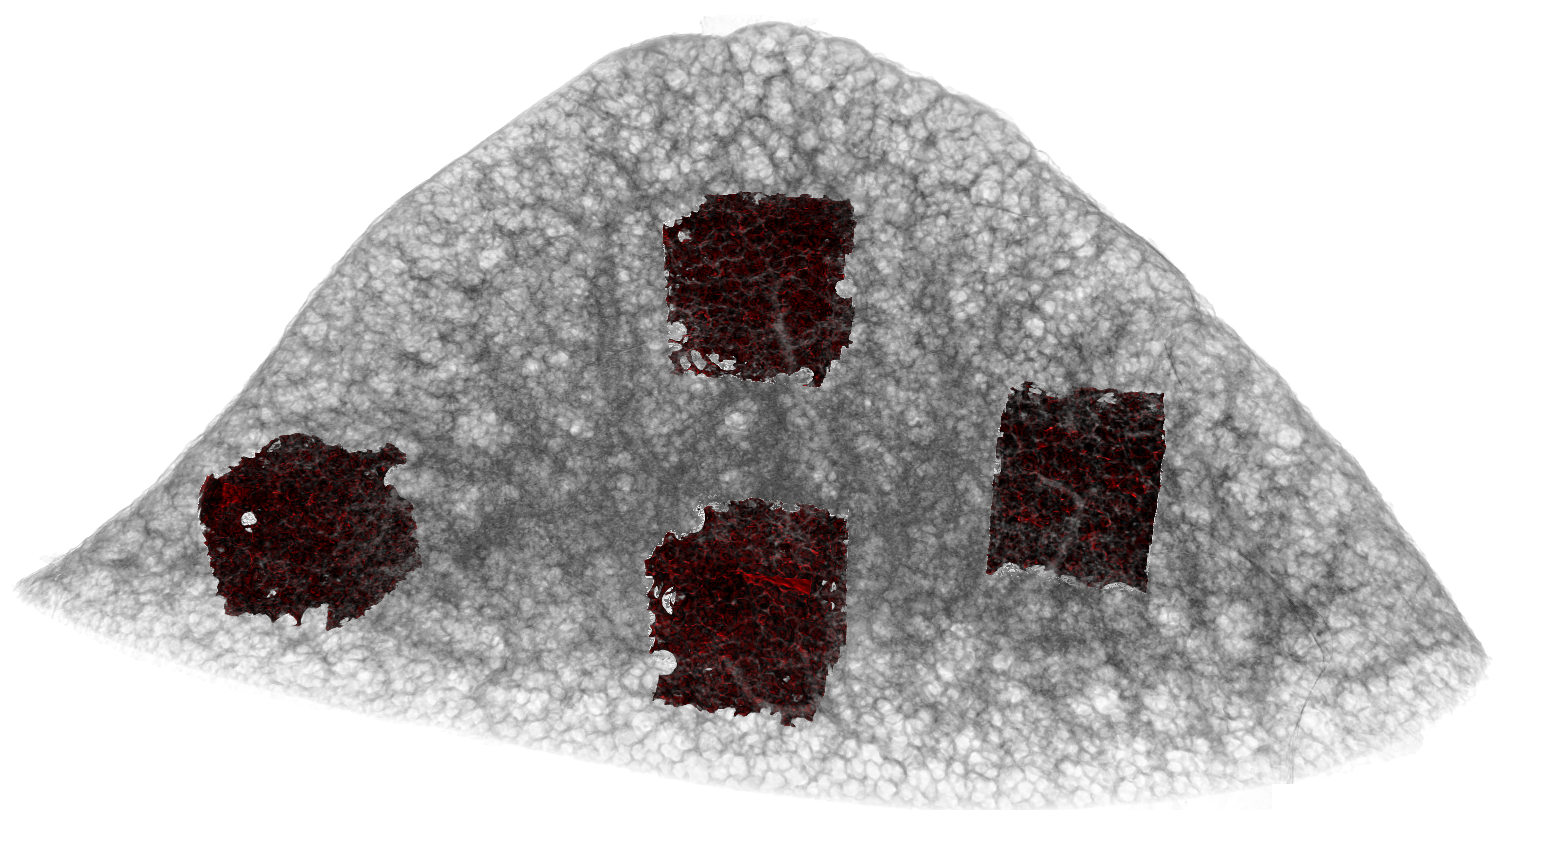
\includegraphics[width=\imagewidth]{img/ROIs-3d}};
		% 1357px = 4.0138mm > 100px = 296um > 169px = 500um
		% \draw[|-|,thick,red] (83,517) -- (1425,719) node [sloped,midway,below] {\SI{4.0138}{\milli\meter} (2712px)};
		\draw[|-|,thick] (\x,\y) -- (\x+169,\y) node [midway, above] {\SI{500}{\micro\meter}};
		%\draw[|-|,thick, white] (\x+645,\y-180) -- (\x+645+128,\y-180) node [midway, below] {\SI{256}{pixels}};
		\draw ( 368,360) node [fill=white, semitransparent] {ROI 1} node {ROI 1};
		\draw (1038,312) node [fill=white, semitransparent] {ROI 2} node {ROI 2};
		\draw ( 767,413) node [fill=white, semitransparent] {ROI 3} node {ROI 3};
		\draw ( 684,139) node [fill=white, semitransparent] {ROI 4} node {ROI 4};
		\end{tikzpicture}%
	\caption{Overview of the placement of the four regions of interest where the histogram of the euclidean distance transformation distribution has been calculated. Grey: Semitransparent volume rendering of the lung tissue sample. Red: Four regions of interest, extracted to calculate the distance transformation, each with a side-length of 256 pixels. The labels of the ROIs conform to the legends in figure~\ref{fig:DTFplots}.}%		
	\label{fig:roi3d}
\end{figure}

For comparison, the histogram of the euclidean distance transformation has been plotted for all four regions of interest in each protocol (B, L and T).

\renewcommand{\imsize}{.309\columnwidth}
\begin{figure}[htp]
	\centering
	\begin{tabular}{cc}
		% \documentclass{article}
% \usepackage{tikz,pgfplots}
% \usepackage[pdftex,active,tightpage]{preview}
% \begin{document}
% \begin{preview}
%%%%%%%%%%%%
\begin{tikzpicture}

% Axis at [0.13 0.11 0.78 0.81]
\begin{semilogyaxis}[
% axis on top,
% scale only axis,
grid=both,
width=\imsize,
% height=3.56562in,
xmin=0, xmax=65,
ymin=1, ymax=1e+007,
xlabel={Thickness [\micro m]},
ylabel={Number of Voxels},
% title={ROI 1},
legend entries={slow (ROI 1),med (ROI 1),fast (ROI 1)}
]

\addplot [
color=blue,
solid
]coordinates{
 (1.036,0) (1.036,1.25111e+006) (1.036,1.25111e+006) (1.184,1.25111e+006) (1.184,0)%
 (1.332,0) (1.332,615061) (1.332,615061) (1.48,615061) (1.48,0)%
 (1.776,0) (1.776,260078) (1.776,260078) (1.924,260078) (1.924,0)%
 (2.072,0) (2.072,311501) (2.072,311501) (2.22,311501) (2.22,487193) (2.22,487193) (2.368,487193) (2.368,0)%
 (2.516,0) (2.516,247233) (2.516,247233) (2.664,247233) (2.664,0)%
 (2.812,0) (2.812,262874) (2.812,262874) (2.96,262874) (2.96,0)%
 (3.108,0) (3.108,362647) (3.108,362647) (3.256,362647) (3.256,177701) (3.256,177701) (3.404,177701) (3.404,143434) (3.404,143434) (3.552,143434) (3.552,73909) (3.552,73909) (3.7,73909) (3.7,216769) (3.7,216769) (3.848,216769) (3.848,205224) (3.848,205224) (3.996,205224) (3.996,0)%
 (4.144,0) (4.144,379292) (4.144,379292) (4.292,379292) (4.292,144948) (4.292,144948) (4.44,144948) (4.44,79396) (4.44,79396) (4.588,79396) (4.588,102403) (4.588,102403) (4.736,102403) (4.736,209710) (4.736,209710) (4.884,209710) (4.884,0)%
 (5.032,0) (5.032,289501) (5.032,289501) (5.18,289501) (5.18,168870) (5.18,168870) (5.328,168870) (5.328,65511) (5.328,65511) (5.476,65511) (5.476,185453) (5.476,185453) (5.624,185453) (5.624,74694) (5.624,74694) (5.772,74694) (5.772,52846) (5.772,52846) (5.92,52846) (5.92,230325) (5.92,230325) (6.068,230325) (6.068,70838) (6.068,70838) (6.216,70838) (6.216,127584) (6.216,127584) (6.364,127584) (6.364,112007) (6.364,112007) (6.512,112007) (6.512,220564) (6.512,220564) (6.66,220564) (6.66,83095) (6.66,83095) (6.808,83095) (6.808,140906) (6.808,140906) (6.956,140906) (6.956,46921) (6.956,46921) (7.104,46921) (7.104,98956) (7.104,98956) (7.252,98956) (7.252,191119) (7.252,191119) (7.4,191119) (7.4,109497) (7.4,109497) (7.548,109497) (7.548,83683) (7.548,83683) (7.696,83683) (7.696,95212) (7.696,95212) (7.844,95212) (7.844,98242) (7.844,98242) (7.992,98242) (7.992,85358) (7.992,85358) (8.14,85358) (8.14,69667) (8.14,69667) (8.288,69667) (8.288,193089) (8.288,193089) (8.436,193089) (8.436,60959) (8.436,60959) (8.584,60959) (8.584,87206) (8.584,87206) (8.732,87206) (8.732,88163) (8.732,88163) (8.88,88163) (8.88,111357) (8.88,111357) (9.028,111357) (9.028,94851) (9.028,94851) (9.176,94851) (9.176,28137) (9.176,28137) (9.324,28137) (9.324,151541) (9.324,151541) (9.472,151541) (9.472,121345) (9.472,121345) (9.62,121345) (9.62,14476) (9.62,14476) (9.768,14476) (9.768,148633) (9.768,148633) (9.916,148633) (9.916,68210) (9.916,68210) (10.064,68210) (10.064,51398) (10.064,51398) (10.212,51398) (10.212,114875) (10.212,114875) (10.36,114875) (10.36,79729) (10.36,79729) (10.508,79729) (10.508,68479) (10.508,68479) (10.656,68479) (10.656,72250) (10.656,72250) (10.804,72250) (10.804,72049) (10.804,72049) (10.952,72049) (10.952,79753) (10.952,79753) (11.1,79753) (11.1,81664) (11.1,81664) (11.248,81664) (11.248,34829) (11.248,34829) (11.396,34829) (11.396,90607) (11.396,90607) (11.544,90607) (11.544,86063) (11.544,86063) (11.692,86063) (11.692,69170) (11.692,69170) (11.84,69170) (11.84,53271) (11.84,53271) (11.988,53271) (11.988,83343) (11.988,83343) (12.136,83343) (12.136,49082) (12.136,49082) (12.284,49082) (12.284,32539) (12.284,32539) (12.432,32539) (12.432,111026) (12.432,111026) (12.58,111026) (12.58,63768) (12.58,63768) (12.728,63768) (12.728,62827) (12.728,62827) (12.876,62827) (12.876,51868) (12.876,51868) (13.024,51868) (13.024,48185) (13.024,48185) (13.172,48185) (13.172,62312) (13.172,62312) (13.32,62312) (13.32,45697) (13.32,45697) (13.468,45697) (13.468,59199) (13.468,59199) (13.616,59199) (13.616,50125) (13.616,50125) (13.764,50125) (13.764,61532) (13.764,61532) (13.912,61532) (13.912,48789) (13.912,48789) (14.06,48789) (14.06,54360) (14.06,54360) (14.208,54360) (14.208,32444) (14.208,32444) (14.356,32444) (14.356,65857) (14.356,65857) (14.504,65857) (14.504,51861) (14.504,51861) (14.652,51861) (14.652,45863) (14.652,45863) (14.8,45863) (14.8,47039) (14.8,47039) (14.948,47039) (14.948,53244) (14.948,53244) (15.096,53244) (15.096,30468) (15.096,30468) (15.244,30468) (15.244,36249) (15.244,36249) (15.392,36249) (15.392,43946) (15.392,43946) (15.54,43946) (15.54,63584) (15.54,63584) (15.688,63584) (15.688,40905) (15.688,40905) (15.836,40905) (15.836,49551) (15.836,49551) (15.984,49551) (15.984,31017) (15.984,31017) (16.132,31017) (16.132,44626) (16.132,44626) (16.28,44626) (16.28,45134) (16.28,45134) (16.428,45134) (16.428,19390) (16.428,19390) (16.576,19390) (16.576,48419) (16.576,48419) (16.724,48419) (16.724,40598) (16.724,40598) (16.872,40598) (16.872,43419) (16.872,43419) (17.02,43419) (17.02,33352) (17.02,33352) (17.168,33352) (17.168,31319) (17.168,31319) (17.316,31319) (17.316,32941) (17.316,32941) (17.464,32941) (17.464,27127) (17.464,27127) (17.612,27127) (17.612,52285) (17.612,52285) (17.76,52285) (17.76,34413) (17.76,34413) (17.908,34413) (17.908,27138) (17.908,27138) (18.056,27138) (18.056,38339) (18.056,38339) (18.204,38339) (18.204,24127) (18.204,24127) (18.352,24127) (18.352,38567) (18.352,38567) (18.5,38567) (18.5,27187) (18.5,27187) (18.648,27187) (18.648,48367) (18.648,48367) (18.796,48367) (18.796,24372) (18.796,24372) (18.944,24372) (18.944,28211) (18.944,28211) (19.092,28211) (19.092,32657) (19.092,32657) (19.24,32657) (19.24,33653) (19.24,33653) (19.388,33653) (19.388,23533) (19.388,23533) (19.536,23533) (19.536,19206) (19.536,19206) (19.684,19206) (19.684,42551) (19.684,42551) (19.832,42551) (19.832,27399) (19.832,27399) (19.98,27399) (19.98,31332) (19.98,31332) (20.128,31332) (20.128,21042) (20.128,21042) (20.276,21042) (20.276,23662) (20.276,23662) (20.424,23662) (20.424,30551) (20.424,30551) (20.572,30551) (20.572,23126) (20.572,23126) (20.72,23126) (20.72,32415) (20.72,32415) (20.868,32415) (20.868,26522) (20.868,26522) (21.016,26522) (21.016,22807) (21.016,22807) (21.164,22807) (21.164,20796) (21.164,20796) (21.312,20796) (21.312,31838) (21.312,31838) (21.46,31838) (21.46,21486) (21.46,21486) (21.608,21486) (21.608,17839) (21.608,17839) (21.756,17839) (21.756,29346) (21.756,29346) (21.904,29346) (21.904,25394) (21.904,25394) (22.052,25394) (22.052,23931) (22.052,23931) (22.2,23931) (22.2,19010) (22.2,19010) (22.348,19010) (22.348,20692) (22.348,20692) (22.496,20692) (22.496,19154) (22.496,19154) (22.644,19154) (22.644,18638) (22.644,18638) (22.792,18638) (22.792,29391) (22.792,29391) (22.94,29391) (22.94,15838) (22.94,15838) (23.088,15838) (23.088,21447) (23.088,21447) (23.236,21447) (23.236,22688) (23.236,22688) (23.384,22688) (23.384,15210) (23.384,15210) (23.532,15210) (23.532,21187) (23.532,21187) (23.68,21187) (23.68,13291) (23.68,13291) (23.828,13291) (23.828,22614) (23.828,22614) (23.976,22614) (23.976,19969) (23.976,19969) (24.124,19969) (24.124,16789) (24.124,16789) (24.272,16789) (24.272,17367) (24.272,17367) (24.42,17367) (24.42,15681) (24.42,15681) (24.568,15681) (24.568,19884) (24.568,19884) (24.716,19884) (24.716,9854) (24.716,9854) (24.864,9854) (24.864,20652) (24.864,20652) (25.012,20652) (25.012,16546) (25.012,16546) (25.16,16546) (25.16,16711) (25.16,16711) (25.308,16711) (25.308,13728) (25.308,13728) (25.456,13728) (25.456,12229) (25.456,12229) (25.604,12229) (25.604,15340) (25.604,15340) (25.752,15340) (25.752,10601) (25.752,10601) (25.9,10601) (25.9,20681) (25.9,20681) (26.048,20681) (26.048,12315) (26.048,12315) (26.196,12315) (26.196,14426) (26.196,14426) (26.344,14426) (26.344,12931) (26.344,12931) (26.492,12931) (26.492,14507) (26.492,14507) (26.64,14507) (26.64,11234) (26.64,11234) (26.788,11234) (26.788,11937) (26.788,11937) (26.936,11937) (26.936,13626) (26.936,13626) (27.084,13626) (27.084,13537) (27.084,13537) (27.232,13537) (27.232,11925) (27.232,11925) (27.38,11925) (27.38,12930) (27.38,12930) (27.528,12930) (27.528,9601) (27.528,9601) (27.676,9601) (27.676,9149) (27.676,9149) (27.824,9149) (27.824,10962) (27.824,10962) (27.972,10962) (27.972,12041) (27.972,12041) (28.12,12041) (28.12,10697) (28.12,10697) (28.268,10697) (28.268,11133) (28.268,11133) (28.416,11133) (28.416,9424) (28.416,9424) (28.564,9424) (28.564,9013) (28.564,9013) (28.712,9013) (28.712,12315) (28.712,12315) (28.86,12315) (28.86,7887) (28.86,7887) (29.008,7887) (29.008,9301) (29.008,9301) (29.156,9301) (29.156,9182) (29.156,9182) (29.304,9182) (29.304,9502) (29.304,9502) (29.452,9502) (29.452,7621) (29.452,7621) (29.6,7621) (29.6,9584) (29.6,9584) (29.748,9584) (29.748,6208) (29.748,6208) (29.896,6208) (29.896,7255) (29.896,7255) (30.044,7255) (30.044,11315) (30.044,11315) (30.192,11315) (30.192,8066) (30.192,8066) (30.34,8066) (30.34,7519) (30.34,7519) (30.488,7519) (30.488,6584) (30.488,6584) (30.636,6584) (30.636,6964) (30.636,6964) (30.784,6964) (30.784,6797) (30.784,6797) (30.932,6797) (30.932,5566) (30.932,5566) (31.08,5566) (31.08,7473) (31.08,7473) (31.228,7473) (31.228,7186) (31.228,7186) (31.376,7186) (31.376,5091) (31.376,5091) (31.524,5091) (31.524,7039) (31.524,7039) (31.672,7039) (31.672,5524) (31.672,5524) (31.82,5524) (31.82,5297) (31.82,5297) (31.968,5297) (31.968,4091) (31.968,4091) (32.116,4091) (32.116,7392) (32.116,7392) (32.264,7392) (32.264,5227) (32.264,5227) (32.412,5227) (32.412,5764) (32.412,5764) (32.56,5764) (32.56,4223) (32.56,4223) (32.708,4223) (32.708,4689) (32.708,4689) (32.856,4689) (32.856,4919) (32.856,4919) (33.004,4919) (33.004,4045) (33.004,4045) (33.152,4045) (33.152,5036) (33.152,5036) (33.3,5036) (33.3,4647) (33.3,4647) (33.448,4647) (33.448,4661) (33.448,4661) (33.596,4661) (33.596,3201) (33.596,3201) (33.744,3201) (33.744,5155) (33.744,5155) (33.892,5155) (33.892,3256) (33.892,3256) (34.04,3256) (34.04,3062) (34.04,3062) (34.188,3062) (34.188,5112) (34.188,5112) (34.336,5112) (34.336,3688) (34.336,3688) (34.484,3688) (34.484,3215) (34.484,3215) (34.632,3215) (34.632,3841) (34.632,3841) (34.78,3841) (34.78,3096) (34.78,3096) (34.928,3096) (34.928,3620) (34.928,3620) (35.076,3620) (35.076,2830) (35.076,2830) (35.224,2830) (35.224,3711) (35.224,3711) (35.372,3711) (35.372,3323) (35.372,3323) (35.52,3323) (35.52,2678) (35.52,2678) (35.668,2678) (35.668,3506) (35.668,3506) (35.816,3506) (35.816,2545) (35.816,2545) (35.964,2545) (35.964,2722) (35.964,2722) (36.112,2722) (36.112,2407) (36.112,2407) (36.26,2407) (36.26,3437) (36.26,3437) (36.408,3437) (36.408,2471) (36.408,2471) (36.556,2471) (36.556,2523) (36.556,2523) (36.704,2523) (36.704,2558) (36.704,2558) (36.852,2558) (36.852,2415) (36.852,2415) (37,2415) (37,1949) (37,1949) (37.148,1949) (37.148,2253) (37.148,2253) (37.296,2253) (37.296,2855) (37.296,2855) (37.444,2855) (37.444,2187) (37.444,2187) (37.592,2187) (37.592,2267) (37.592,2267) (37.74,2267) (37.74,1759) (37.74,1759) (37.888,1759) (37.888,1684) (37.888,1684) (38.036,1684) (38.036,2203) (38.036,2203) (38.184,2203) (38.184,1671) (38.184,1671) (38.332,1671) (38.332,2267) (38.332,2267) (38.48,2267) (38.48,2018) (38.48,2018) (38.628,2018) (38.628,1378) (38.628,1378) (38.776,1378) (38.776,1776) (38.776,1776) (38.924,1776) (38.924,1973) (38.924,1973) (39.072,1973) (39.072,1539) (39.072,1539) (39.22,1539) (39.22,1075) (39.22,1075) (39.368,1075) (39.368,2143) (39.368,2143) (39.516,2143) (39.516,1159) (39.516,1159) (39.664,1159) (39.664,1639) (39.664,1639) (39.812,1639) (39.812,1331) (39.812,1331) (39.96,1331) (39.96,1411) (39.96,1411) (40.108,1411) (40.108,1181) (40.108,1181) (40.256,1181) (40.256,1310) (40.256,1310) (40.404,1310) (40.404,1538) (40.404,1538) (40.552,1538) (40.552,1074) (40.552,1074) (40.7,1074) (40.7,1274) (40.7,1274) (40.848,1274) (40.848,989) (40.848,989) (40.996,989) (40.996,1195) (40.996,1195) (41.144,1195) (41.144,906) (41.144,906) (41.292,906) (41.292,1026) (41.292,1026) (41.44,1026) (41.44,1201) (41.44,1201) (41.588,1201) (41.588,959) (41.588,959) (41.736,959) (41.736,987) (41.736,987) (41.884,987) (41.884,924) (41.884,924) (42.032,924) (42.032,667) (42.032,667) (42.18,667) (42.18,941) (42.18,941) (42.328,941) (42.328,544) (42.328,544) (42.476,544) (42.476,1026) (42.476,1026) (42.624,1026) (42.624,842) (42.624,842) (42.772,842) (42.772,726) (42.772,726) (42.92,726) (42.92,573) (42.92,573) (43.068,573) (43.068,717) (43.068,717) (43.216,717) (43.216,638) (43.216,638) (43.364,638) (43.364,597) (43.364,597) (43.512,597) (43.512,693) (43.512,693) (43.66,693) (43.66,657) (43.66,657) (43.808,657) (43.808,480) (43.808,480) (43.956,480) (43.956,673) (43.956,673) (44.104,673) (44.104,466) (44.104,466) (44.252,466) (44.252,580) (44.252,580) (44.4,580) (44.4,414) (44.4,414) (44.548,414) (44.548,657) (44.548,657) (44.696,657) (44.696,454) (44.696,454) (44.844,454) (44.844,591) (44.844,591) (44.992,591) (44.992,422) (44.992,422) (45.14,422) (45.14,428) (45.14,428) (45.288,428) (45.288,353) (45.288,353) (45.436,353) (45.436,452) (45.436,452) (45.584,452) (45.584,483) (45.584,483) (45.732,483) (45.732,413) (45.732,413) (45.88,413) (45.88,411) (45.88,411) (46.028,411) (46.028,320) (46.028,320) (46.176,320) (46.176,397) (46.176,397) (46.324,397) (46.324,359) (46.324,359) (46.472,359) (46.472,305) (46.472,305) (46.62,305) (46.62,328) (46.62,328) (46.768,328) (46.768,358) (46.768,358) (46.916,358) (46.916,319) (46.916,319) (47.064,319) (47.064,291) (47.064,291) (47.212,291) (47.212,284) (47.212,284) (47.36,284) (47.36,234) (47.36,234) (47.508,234) (47.508,220) (47.508,220) (47.656,220) (47.656,344) (47.656,344) (47.804,344) (47.804,265) (47.804,265) (47.952,265) (47.952,191) (47.952,191) (48.1,191) (48.1,161) (48.1,161) (48.248,161) (48.248,231) (48.248,231) (48.396,231) (48.396,155) (48.396,155) (48.544,155) (48.544,171) (48.544,171) (48.692,171) (48.692,234) (48.692,234) (48.84,234) (48.84,129) (48.84,129) (48.988,129) (48.988,116) (48.988,116) (49.136,116) (49.136,157) (49.136,157) (49.284,157) (49.284,116) (49.284,116) (49.432,116) (49.432,88) (49.432,88) (49.58,88) (49.58,85) (49.58,85) (49.728,85) (49.728,96) (49.728,96) (49.876,96) (49.876,80) (49.876,80) (50.024,80) (50.024,82) (50.024,82) (50.172,82) (50.172,57) (50.172,57) (50.32,57) (50.32,35) (50.32,35) (50.468,35) (50.468,46) (50.468,46) (50.616,46) (50.616,36) (50.616,36) (50.764,36) (50.764,29) (50.764,29) (50.912,29) (50.912,21) (50.912,21) (51.06,21) (51.06,16) (51.06,16) (51.208,16) (51.208,16) (51.208,16) (51.356,16) (51.356,14) (51.356,14) (51.504,14) (51.504,9) (51.504,9) (51.652,9) (51.652,9) (51.652,9) (51.8,9) (51.8,10) (51.8,10) (51.948,10) (51.948,4) (51.948,4) (52.096,4) (52.096,4) (52.096,4) (52.244,4) (52.244,2) (52.244,2) (52.392,2) (52.392,1)%
 (52.54,1) (52.54,2) (52.54,2) (52.688,2) (52.688,1)
};

\addplot [
color=green,
solid
]coordinates{
 (1.036,0) (1.036,1.25308e+006) (1.036,1.25308e+006) (1.184,1.25308e+006) (1.184,0)%
 (1.332,0) (1.332,613821) (1.332,613821) (1.48,613821) (1.48,0)%
 (1.776,0) (1.776,259899) (1.776,259899) (1.924,259899) (1.924,0)%
 (2.072,0) (2.072,310370) (2.072,310370) (2.22,310370) (2.22,486829) (2.22,486829) (2.368,486829) (2.368,0)%
 (2.516,0) (2.516,247747) (2.516,247747) (2.664,247747) (2.664,0)%
 (2.812,0) (2.812,258533) (2.812,258533) (2.96,258533) (2.96,0)%
 (3.108,0) (3.108,361745) (3.108,361745) (3.256,361745) (3.256,179371) (3.256,179371) (3.404,179371) (3.404,143506) (3.404,143506) (3.552,143506) (3.552,72869) (3.552,72869) (3.7,72869) (3.7,214163) (3.7,214163) (3.848,214163) (3.848,206273) (3.848,206273) (3.996,206273) (3.996,0)%
 (4.144,0) (4.144,376367) (4.144,376367) (4.292,376367) (4.292,144871) (4.292,144871) (4.44,144871) (4.44,79489) (4.44,79489) (4.588,79489) (4.588,101729) (4.588,101729) (4.736,101729) (4.736,209144) (4.736,209144) (4.884,209144) (4.884,0)%
 (5.032,0) (5.032,285587) (5.032,285587) (5.18,285587) (5.18,169714) (5.18,169714) (5.328,169714) (5.328,65682) (5.328,65682) (5.476,65682) (5.476,183620) (5.476,183620) (5.624,183620) (5.624,75379) (5.624,75379) (5.772,75379) (5.772,51642) (5.772,51642) (5.92,51642) (5.92,227882) (5.92,227882) (6.068,227882) (6.068,71053) (6.068,71053) (6.216,71053) (6.216,127295) (6.216,127295) (6.364,127295) (6.364,111638) (6.364,111638) (6.512,111638) (6.512,218480) (6.512,218480) (6.66,218480) (6.66,82720) (6.66,82720) (6.808,82720) (6.808,139178) (6.808,139178) (6.956,139178) (6.956,47263) (6.956,47263) (7.104,47263) (7.104,97436) (7.104,97436) (7.252,97436) (7.252,190870) (7.252,190870) (7.4,190870) (7.4,108250) (7.4,108250) (7.548,108250) (7.548,83492) (7.548,83492) (7.696,83492) (7.696,94695) (7.696,94695) (7.844,94695) (7.844,96844) (7.844,96844) (7.992,96844) (7.992,84074) (7.992,84074) (8.14,84074) (8.14,69652) (8.14,69652) (8.288,69652) (8.288,191832) (8.288,191832) (8.436,191832) (8.436,60244) (8.436,60244) (8.584,60244) (8.584,86981) (8.584,86981) (8.732,86981) (8.732,86728) (8.732,86728) (8.88,86728) (8.88,110216) (8.88,110216) (9.028,110216) (9.028,94312) (9.028,94312) (9.176,94312) (9.176,27164) (9.176,27164) (9.324,27164) (9.324,150953) (9.324,150953) (9.472,150953) (9.472,120343) (9.472,120343) (9.62,120343) (9.62,14202) (9.62,14202) (9.768,14202) (9.768,147009) (9.768,147009) (9.916,147009) (9.916,67351) (9.916,67351) (10.064,67351) (10.064,49810) (10.064,49810) (10.212,49810) (10.212,114108) (10.212,114108) (10.36,114108) (10.36,79775) (10.36,79775) (10.508,79775) (10.508,67677) (10.508,67677) (10.656,67677) (10.656,71054) (10.656,71054) (10.804,71054) (10.804,71112) (10.804,71112) (10.952,71112) (10.952,78892) (10.952,78892) (11.1,78892) (11.1,80222) (11.1,80222) (11.248,80222) (11.248,34643) (11.248,34643) (11.396,34643) (11.396,90088) (11.396,90088) (11.544,90088) (11.544,84851) (11.544,84851) (11.692,84851) (11.692,68051) (11.692,68051) (11.84,68051) (11.84,52909) (11.84,52909) (11.988,52909) (11.988,81863) (11.988,81863) (12.136,81863) (12.136,48703) (12.136,48703) (12.284,48703) (12.284,32105) (12.284,32105) (12.432,32105) (12.432,109750) (12.432,109750) (12.58,109750) (12.58,63514) (12.58,63514) (12.728,63514) (12.728,62172) (12.728,62172) (12.876,62172) (12.876,50881) (12.876,50881) (13.024,50881) (13.024,47091) (13.024,47091) (13.172,47091) (13.172,62039) (13.172,62039) (13.32,62039) (13.32,44968) (13.32,44968) (13.468,44968) (13.468,58587) (13.468,58587) (13.616,58587) (13.616,49966) (13.616,49966) (13.764,49966) (13.764,60443) (13.764,60443) (13.912,60443) (13.912,48528) (13.912,48528) (14.06,48528) (14.06,53901) (14.06,53901) (14.208,53901) (14.208,32302) (14.208,32302) (14.356,32302) (14.356,64503) (14.356,64503) (14.504,64503) (14.504,51449) (14.504,51449) (14.652,51449) (14.652,45907) (14.652,45907) (14.8,45907) (14.8,46182) (14.8,46182) (14.948,46182) (14.948,52795) (14.948,52795) (15.096,52795) (15.096,30334) (15.096,30334) (15.244,30334) (15.244,35498) (15.244,35498) (15.392,35498) (15.392,43463) (15.392,43463) (15.54,43463) (15.54,63129) (15.54,63129) (15.688,63129) (15.688,40290) (15.688,40290) (15.836,40290) (15.836,49459) (15.836,49459) (15.984,49459) (15.984,30485) (15.984,30485) (16.132,30485) (16.132,44159) (16.132,44159) (16.28,44159) (16.28,44784) (16.28,44784) (16.428,44784) (16.428,19043) (16.428,19043) (16.576,19043) (16.576,48026) (16.576,48026) (16.724,48026) (16.724,40100) (16.724,40100) (16.872,40100) (16.872,43361) (16.872,43361) (17.02,43361) (17.02,33092) (17.02,33092) (17.168,33092) (17.168,30961) (17.168,30961) (17.316,30961) (17.316,32607) (17.316,32607) (17.464,32607) (17.464,26918) (17.464,26918) (17.612,26918) (17.612,51725) (17.612,51725) (17.76,51725) (17.76,34420) (17.76,34420) (17.908,34420) (17.908,27015) (17.908,27015) (18.056,27015) (18.056,37899) (18.056,37899) (18.204,37899) (18.204,23839) (18.204,23839) (18.352,23839) (18.352,38670) (18.352,38670) (18.5,38670) (18.5,26977) (18.5,26977) (18.648,26977) (18.648,47886) (18.648,47886) (18.796,47886) (18.796,24290) (18.796,24290) (18.944,24290) (18.944,27865) (18.944,27865) (19.092,27865) (19.092,32681) (19.092,32681) (19.24,32681) (19.24,33349) (19.24,33349) (19.388,33349) (19.388,23303) (19.388,23303) (19.536,23303) (19.536,19055) (19.536,19055) (19.684,19055) (19.684,42280) (19.684,42280) (19.832,42280) (19.832,27188) (19.832,27188) (19.98,27188) (19.98,31068) (19.98,31068) (20.128,31068) (20.128,20995) (20.128,20995) (20.276,20995) (20.276,23250) (20.276,23250) (20.424,23250) (20.424,30452) (20.424,30452) (20.572,30452) (20.572,23216) (20.572,23216) (20.72,23216) (20.72,31851) (20.72,31851) (20.868,31851) (20.868,26262) (20.868,26262) (21.016,26262) (21.016,22485) (21.016,22485) (21.164,22485) (21.164,20842) (21.164,20842) (21.312,20842) (21.312,31568) (21.312,31568) (21.46,31568) (21.46,21410) (21.46,21410) (21.608,21410) (21.608,17685) (21.608,17685) (21.756,17685) (21.756,28680) (21.756,28680) (21.904,28680) (21.904,25232) (21.904,25232) (22.052,25232) (22.052,23625) (22.052,23625) (22.2,23625) (22.2,18840) (22.2,18840) (22.348,18840) (22.348,20349) (22.348,20349) (22.496,20349) (22.496,18791) (22.496,18791) (22.644,18791) (22.644,18512) (22.644,18512) (22.792,18512) (22.792,28981) (22.792,28981) (22.94,28981) (22.94,15601) (22.94,15601) (23.088,15601) (23.088,20967) (23.088,20967) (23.236,20967) (23.236,22281) (23.236,22281) (23.384,22281) (23.384,15077) (23.384,15077) (23.532,15077) (23.532,20798) (23.532,20798) (23.68,20798) (23.68,13211) (23.68,13211) (23.828,13211) (23.828,22204) (23.828,22204) (23.976,22204) (23.976,19528) (23.976,19528) (24.124,19528) (24.124,16521) (24.124,16521) (24.272,16521) (24.272,17226) (24.272,17226) (24.42,17226) (24.42,15381) (24.42,15381) (24.568,15381) (24.568,19527) (24.568,19527) (24.716,19527) (24.716,9783) (24.716,9783) (24.864,9783) (24.864,20502) (24.864,20502) (25.012,20502) (25.012,16286) (25.012,16286) (25.16,16286) (25.16,16331) (25.16,16331) (25.308,16331) (25.308,13462) (25.308,13462) (25.456,13462) (25.456,11926) (25.456,11926) (25.604,11926) (25.604,15227) (25.604,15227) (25.752,15227) (25.752,10583) (25.752,10583) (25.9,10583) (25.9,20302) (25.9,20302) (26.048,20302) (26.048,11984) (26.048,11984) (26.196,11984) (26.196,13994) (26.196,13994) (26.344,13994) (26.344,12825) (26.344,12825) (26.492,12825) (26.492,14359) (26.492,14359) (26.64,14359) (26.64,11078) (26.64,11078) (26.788,11078) (26.788,11732) (26.788,11732) (26.936,11732) (26.936,13287) (26.936,13287) (27.084,13287) (27.084,13401) (27.084,13401) (27.232,13401) (27.232,11693) (27.232,11693) (27.38,11693) (27.38,12642) (27.38,12642) (27.528,12642) (27.528,9455) (27.528,9455) (27.676,9455) (27.676,8944) (27.676,8944) (27.824,8944) (27.824,10839) (27.824,10839) (27.972,10839) (27.972,11862) (27.972,11862) (28.12,11862) (28.12,10426) (28.12,10426) (28.268,10426) (28.268,10817) (28.268,10817) (28.416,10817) (28.416,9237) (28.416,9237) (28.564,9237) (28.564,8842) (28.564,8842) (28.712,8842) (28.712,12068) (28.712,12068) (28.86,12068) (28.86,7734) (28.86,7734) (29.008,7734) (29.008,9009) (29.008,9009) (29.156,9009) (29.156,8824) (29.156,8824) (29.304,8824) (29.304,9234) (29.304,9234) (29.452,9234) (29.452,7496) (29.452,7496) (29.6,7496) (29.6,9337) (29.6,9337) (29.748,9337) (29.748,6054) (29.748,6054) (29.896,6054) (29.896,7045) (29.896,7045) (30.044,7045) (30.044,11020) (30.044,11020) (30.192,11020) (30.192,7832) (30.192,7832) (30.34,7832) (30.34,7268) (30.34,7268) (30.488,7268) (30.488,6314) (30.488,6314) (30.636,6314) (30.636,6675) (30.636,6675) (30.784,6675) (30.784,6701) (30.784,6701) (30.932,6701) (30.932,5453) (30.932,5453) (31.08,5453) (31.08,7241) (31.08,7241) (31.228,7241) (31.228,6856) (31.228,6856) (31.376,6856) (31.376,4903) (31.376,4903) (31.524,4903) (31.524,6899) (31.524,6899) (31.672,6899) (31.672,5384) (31.672,5384) (31.82,5384) (31.82,5093) (31.82,5093) (31.968,5093) (31.968,3919) (31.968,3919) (32.116,3919) (32.116,7087) (32.116,7087) (32.264,7087) (32.264,5140) (32.264,5140) (32.412,5140) (32.412,5584) (32.412,5584) (32.56,5584) (32.56,4113) (32.56,4113) (32.708,4113) (32.708,4524) (32.708,4524) (32.856,4524) (32.856,4706) (32.856,4706) (33.004,4706) (33.004,3951) (33.004,3951) (33.152,3951) (33.152,4904) (33.152,4904) (33.3,4904) (33.3,4486) (33.3,4486) (33.448,4486) (33.448,4478) (33.448,4478) (33.596,4478) (33.596,3105) (33.596,3105) (33.744,3105) (33.744,4990) (33.744,4990) (33.892,4990) (33.892,3121) (33.892,3121) (34.04,3121) (34.04,2940) (34.04,2940) (34.188,2940) (34.188,4888) (34.188,4888) (34.336,4888) (34.336,3596) (34.336,3596) (34.484,3596) (34.484,3131) (34.484,3131) (34.632,3131) (34.632,3638) (34.632,3638) (34.78,3638) (34.78,2989) (34.78,2989) (34.928,2989) (34.928,3418) (34.928,3418) (35.076,3418) (35.076,2727) (35.076,2727) (35.224,2727) (35.224,3595) (35.224,3595) (35.372,3595) (35.372,3212) (35.372,3212) (35.52,3212) (35.52,2540) (35.52,2540) (35.668,2540) (35.668,3348) (35.668,3348) (35.816,3348) (35.816,2493) (35.816,2493) (35.964,2493) (35.964,2621) (35.964,2621) (36.112,2621) (36.112,2243) (36.112,2243) (36.26,2243) (36.26,3329) (36.26,3329) (36.408,3329) (36.408,2395) (36.408,2395) (36.556,2395) (36.556,2465) (36.556,2465) (36.704,2465) (36.704,2478) (36.704,2478) (36.852,2478) (36.852,2275) (36.852,2275) (37,2275) (37,1818) (37,1818) (37.148,1818) (37.148,2114) (37.148,2114) (37.296,2114) (37.296,2792) (37.296,2792) (37.444,2792) (37.444,2130) (37.444,2130) (37.592,2130) (37.592,2147) (37.592,2147) (37.74,2147) (37.74,1690) (37.74,1690) (37.888,1690) (37.888,1572) (37.888,1572) (38.036,1572) (38.036,2162) (38.036,2162) (38.184,2162) (38.184,1563) (38.184,1563) (38.332,1563) (38.332,2129) (38.332,2129) (38.48,2129) (38.48,1893) (38.48,1893) (38.628,1893) (38.628,1346) (38.628,1346) (38.776,1346) (38.776,1765) (38.776,1765) (38.924,1765) (38.924,1829) (38.924,1829) (39.072,1829) (39.072,1439) (39.072,1439) (39.22,1439) (39.22,1003) (39.22,1003) (39.368,1003) (39.368,2001) (39.368,2001) (39.516,2001) (39.516,1149) (39.516,1149) (39.664,1149) (39.664,1565) (39.664,1565) (39.812,1565) (39.812,1226) (39.812,1226) (39.96,1226) (39.96,1335) (39.96,1335) (40.108,1335) (40.108,1065) (40.108,1065) (40.256,1065) (40.256,1313) (40.256,1313) (40.404,1313) (40.404,1425) (40.404,1425) (40.552,1425) (40.552,1005) (40.552,1005) (40.7,1005) (40.7,1165) (40.7,1165) (40.848,1165) (40.848,931) (40.848,931) (40.996,931) (40.996,1177) (40.996,1177) (41.144,1177) (41.144,841) (41.144,841) (41.292,841) (41.292,968) (41.292,968) (41.44,968) (41.44,1062) (41.44,1062) (41.588,1062) (41.588,884) (41.588,884) (41.736,884) (41.736,990) (41.736,990) (41.884,990) (41.884,827) (41.884,827) (42.032,827) (42.032,621) (42.032,621) (42.18,621) (42.18,851) (42.18,851) (42.328,851) (42.328,512) (42.328,512) (42.476,512) (42.476,965) (42.476,965) (42.624,965) (42.624,779) (42.624,779) (42.772,779) (42.772,624) (42.772,624) (42.92,624) (42.92,522) (42.92,522) (43.068,522) (43.068,649) (43.068,649) (43.216,649) (43.216,679) (43.216,679) (43.364,679) (43.364,548) (43.364,548) (43.512,548) (43.512,629) (43.512,629) (43.66,629) (43.66,569) (43.66,569) (43.808,569) (43.808,484) (43.808,484) (43.956,484) (43.956,638) (43.956,638) (44.104,638) (44.104,410) (44.104,410) (44.252,410) (44.252,512) (44.252,512) (44.4,512) (44.4,371) (44.4,371) (44.548,371) (44.548,640) (44.548,640) (44.696,640) (44.696,418) (44.696,418) (44.844,418) (44.844,511) (44.844,511) (44.992,511) (44.992,364) (44.992,364) (45.14,364) (45.14,393) (45.14,393) (45.288,393) (45.288,373) (45.288,373) (45.436,373) (45.436,426) (45.436,426) (45.584,426) (45.584,414) (45.584,414) (45.732,414) (45.732,353) (45.732,353) (45.88,353) (45.88,355) (45.88,355) (46.028,355) (46.028,367) (46.028,367) (46.176,367) (46.176,348) (46.176,348) (46.324,348) (46.324,322) (46.324,322) (46.472,322) (46.472,267) (46.472,267) (46.62,267) (46.62,289) (46.62,289) (46.768,289) (46.768,362) (46.768,362) (46.916,362) (46.916,311) (46.916,311) (47.064,311) (47.064,240) (47.064,240) (47.212,240) (47.212,233) (47.212,233) (47.36,233) (47.36,221) (47.36,221) (47.508,221) (47.508,242) (47.508,242) (47.656,242) (47.656,326) (47.656,326) (47.804,326) (47.804,214) (47.804,214) (47.952,214) (47.952,165) (47.952,165) (48.1,165) (48.1,144) (48.1,144) (48.248,144) (48.248,254) (48.248,254) (48.396,254) (48.396,133) (48.396,133) (48.544,133) (48.544,143) (48.544,143) (48.692,143) (48.692,206) (48.692,206) (48.84,206) (48.84,112) (48.84,112) (48.988,112) (48.988,130) (48.988,130) (49.136,130) (49.136,133) (49.136,133) (49.284,133) (49.284,98) (49.284,98) (49.432,98) (49.432,74) (49.432,74) (49.58,74) (49.58,88) (49.58,88) (49.728,88) (49.728,104) (49.728,104) (49.876,104) (49.876,79) (49.876,79) (50.024,79) (50.024,79) (50.024,79) (50.172,79) (50.172,49) (50.172,49) (50.32,49) (50.32,35) (50.32,35) (50.468,35) (50.468,61) (50.468,61) (50.616,61) (50.616,52) (50.616,52) (50.764,52) (50.764,26) (50.764,26) (50.912,26) (50.912,26) (50.912,26) (51.06,26) (51.06,14) (51.06,14) (51.208,14) (51.208,11) (51.208,11) (51.356,11) (51.356,14) (51.356,14) (51.504,14) (51.504,11) (51.504,11) (51.652,11) (51.652,9) (51.652,9) (51.8,9) (51.8,4) (51.8,4) (51.948,4) (51.948,2) (51.948,2) (52.096,2) (52.096,4) (52.096,4) (52.244,4) (52.244,1)
};

\addplot [
color=red,
solid
]coordinates{
 (1.036,0) (1.036,1.24122e+006) (1.036,1.24122e+006) (1.184,1.24122e+006) (1.184,0)%
 (1.332,0) (1.332,611739) (1.332,611739) (1.48,611739) (1.48,0)%
 (1.776,0) (1.776,256848) (1.776,256848) (1.924,256848) (1.924,0)%
 (2.072,0) (2.072,306567) (2.072,306567) (2.22,306567) (2.22,487001) (2.22,487001) (2.368,487001) (2.368,0)%
 (2.516,0) (2.516,247011) (2.516,247011) (2.664,247011) (2.664,0)%
 (2.812,0) (2.812,255784) (2.812,255784) (2.96,255784) (2.96,0)%
 (3.108,0) (3.108,358741) (3.108,358741) (3.256,358741) (3.256,180353) (3.256,180353) (3.404,180353) (3.404,142096) (3.404,142096) (3.552,142096) (3.552,71531) (3.552,71531) (3.7,71531) (3.7,213489) (3.7,213489) (3.848,213489) (3.848,207257) (3.848,207257) (3.996,207257) (3.996,0)%
 (4.144,0) (4.144,370952) (4.144,370952) (4.292,370952) (4.292,144516) (4.292,144516) (4.44,144516) (4.44,79775) (4.44,79775) (4.588,79775) (4.588,101814) (4.588,101814) (4.736,101814) (4.736,208291) (4.736,208291) (4.884,208291) (4.884,0)%
 (5.032,0) (5.032,280054) (5.032,280054) (5.18,280054) (5.18,171184) (5.18,171184) (5.328,171184) (5.328,65309) (5.328,65309) (5.476,65309) (5.476,182699) (5.476,182699) (5.624,182699) (5.624,75927) (5.624,75927) (5.772,75927) (5.772,50874) (5.772,50874) (5.92,50874) (5.92,225669) (5.92,225669) (6.068,225669) (6.068,71324) (6.068,71324) (6.216,71324) (6.216,125610) (6.216,125610) (6.364,125610) (6.364,110775) (6.364,110775) (6.512,110775) (6.512,217173) (6.512,217173) (6.66,217173) (6.66,83148) (6.66,83148) (6.808,83148) (6.808,138194) (6.808,138194) (6.956,138194) (6.956,47473) (6.956,47473) (7.104,47473) (7.104,94945) (7.104,94945) (7.252,94945) (7.252,189881) (7.252,189881) (7.4,189881) (7.4,108607) (7.4,108607) (7.548,108607) (7.548,83005) (7.548,83005) (7.696,83005) (7.696,93773) (7.696,93773) (7.844,93773) (7.844,96586) (7.844,96586) (7.992,96586) (7.992,83114) (7.992,83114) (8.14,83114) (8.14,70267) (8.14,70267) (8.288,70267) (8.288,189486) (8.288,189486) (8.436,189486) (8.436,60420) (8.436,60420) (8.584,60420) (8.584,87028) (8.584,87028) (8.732,87028) (8.732,85112) (8.732,85112) (8.88,85112) (8.88,110338) (8.88,110338) (9.028,110338) (9.028,94578) (9.028,94578) (9.176,94578) (9.176,26972) (9.176,26972) (9.324,26972) (9.324,148780) (9.324,148780) (9.472,148780) (9.472,120400) (9.472,120400) (9.62,120400) (9.62,14005) (9.62,14005) (9.768,14005) (9.768,147252) (9.768,147252) (9.916,147252) (9.916,66761) (9.916,66761) (10.064,66761) (10.064,49128) (10.064,49128) (10.212,49128) (10.212,112913) (10.212,112913) (10.36,112913) (10.36,79889) (10.36,79889) (10.508,79889) (10.508,67465) (10.508,67465) (10.656,67465) (10.656,70434) (10.656,70434) (10.804,70434) (10.804,71865) (10.804,71865) (10.952,71865) (10.952,77749) (10.952,77749) (11.1,77749) (11.1,80395) (11.1,80395) (11.248,80395) (11.248,34699) (11.248,34699) (11.396,34699) (11.396,88827) (11.396,88827) (11.544,88827) (11.544,84991) (11.544,84991) (11.692,84991) (11.692,67236) (11.692,67236) (11.84,67236) (11.84,52935) (11.84,52935) (11.988,52935) (11.988,81867) (11.988,81867) (12.136,81867) (12.136,48486) (12.136,48486) (12.284,48486) (12.284,32440) (12.284,32440) (12.432,32440) (12.432,107925) (12.432,107925) (12.58,107925) (12.58,63610) (12.58,63610) (12.728,63610) (12.728,62017) (12.728,62017) (12.876,62017) (12.876,50735) (12.876,50735) (13.024,50735) (13.024,46844) (13.024,46844) (13.172,46844) (13.172,61755) (13.172,61755) (13.32,61755) (13.32,44772) (13.32,44772) (13.468,44772) (13.468,58048) (13.468,58048) (13.616,58048) (13.616,50042) (13.616,50042) (13.764,50042) (13.764,59595) (13.764,59595) (13.912,59595) (13.912,48239) (13.912,48239) (14.06,48239) (14.06,53910) (14.06,53910) (14.208,53910) (14.208,32100) (14.208,32100) (14.356,32100) (14.356,64608) (14.356,64608) (14.504,64608) (14.504,50665) (14.504,50665) (14.652,50665) (14.652,45218) (14.652,45218) (14.8,45218) (14.8,46311) (14.8,46311) (14.948,46311) (14.948,52522) (14.948,52522) (15.096,52522) (15.096,29993) (15.096,29993) (15.244,29993) (15.244,35625) (15.244,35625) (15.392,35625) (15.392,43374) (15.392,43374) (15.54,43374) (15.54,62391) (15.54,62391) (15.688,62391) (15.688,40010) (15.688,40010) (15.836,40010) (15.836,49448) (15.836,49448) (15.984,49448) (15.984,30109) (15.984,30109) (16.132,30109) (16.132,44171) (16.132,44171) (16.28,44171) (16.28,44900) (16.28,44900) (16.428,44900) (16.428,19190) (16.428,19190) (16.576,19190) (16.576,47164) (16.576,47164) (16.724,47164) (16.724,39854) (16.724,39854) (16.872,39854) (16.872,43109) (16.872,43109) (17.02,43109) (17.02,33065) (17.02,33065) (17.168,33065) (17.168,30962) (17.168,30962) (17.316,30962) (17.316,32565) (17.316,32565) (17.464,32565) (17.464,26705) (17.464,26705) (17.612,26705) (17.612,50974) (17.612,50974) (17.76,50974) (17.76,33960) (17.76,33960) (17.908,33960) (17.908,26936) (17.908,26936) (18.056,26936) (18.056,37556) (18.056,37556) (18.204,37556) (18.204,23425) (18.204,23425) (18.352,23425) (18.352,38685) (18.352,38685) (18.5,38685) (18.5,26402) (18.5,26402) (18.648,26402) (18.648,47367) (18.648,47367) (18.796,47367) (18.796,23932) (18.796,23932) (18.944,23932) (18.944,27267) (18.944,27267) (19.092,27267) (19.092,32646) (19.092,32646) (19.24,32646) (19.24,33347) (19.24,33347) (19.388,33347) (19.388,22926) (19.388,22926) (19.536,22926) (19.536,18891) (19.536,18891) (19.684,18891) (19.684,41519) (19.684,41519) (19.832,41519) (19.832,26825) (19.832,26825) (19.98,26825) (19.98,30932) (19.98,30932) (20.128,30932) (20.128,21040) (20.128,21040) (20.276,21040) (20.276,22921) (20.276,22921) (20.424,22921) (20.424,30192) (20.424,30192) (20.572,30192) (20.572,22907) (20.572,22907) (20.72,22907) (20.72,31504) (20.72,31504) (20.868,31504) (20.868,25954) (20.868,25954) (21.016,25954) (21.016,22446) (21.016,22446) (21.164,22446) (21.164,20597) (21.164,20597) (21.312,20597) (21.312,31423) (21.312,31423) (21.46,31423) (21.46,21158) (21.46,21158) (21.608,21158) (21.608,17484) (21.608,17484) (21.756,17484) (21.756,28136) (21.756,28136) (21.904,28136) (21.904,25151) (21.904,25151) (22.052,25151) (22.052,23372) (22.052,23372) (22.2,23372) (22.2,18847) (22.2,18847) (22.348,18847) (22.348,20331) (22.348,20331) (22.496,20331) (22.496,18843) (22.496,18843) (22.644,18843) (22.644,18097) (22.644,18097) (22.792,18097) (22.792,28535) (22.792,28535) (22.94,28535) (22.94,15599) (22.94,15599) (23.088,15599) (23.088,20928) (23.088,20928) (23.236,20928) (23.236,22242) (23.236,22242) (23.384,22242) (23.384,14866) (23.384,14866) (23.532,14866) (23.532,20871) (23.532,20871) (23.68,20871) (23.68,13127) (23.68,13127) (23.828,13127) (23.828,21827) (23.828,21827) (23.976,21827) (23.976,19383) (23.976,19383) (24.124,19383) (24.124,16522) (24.124,16522) (24.272,16522) (24.272,17288) (24.272,17288) (24.42,17288) (24.42,15293) (24.42,15293) (24.568,15293) (24.568,19619) (24.568,19619) (24.716,19619) (24.716,9711) (24.716,9711) (24.864,9711) (24.864,20198) (24.864,20198) (25.012,20198) (25.012,16144) (25.012,16144) (25.16,16144) (25.16,16487) (25.16,16487) (25.308,16487) (25.308,13612) (25.308,13612) (25.456,13612) (25.456,11957) (25.456,11957) (25.604,11957) (25.604,15045) (25.604,15045) (25.752,15045) (25.752,10674) (25.752,10674) (25.9,10674) (25.9,20152) (25.9,20152) (26.048,20152) (26.048,12106) (26.048,12106) (26.196,12106) (26.196,14099) (26.196,14099) (26.344,14099) (26.344,12757) (26.344,12757) (26.492,12757) (26.492,14360) (26.492,14360) (26.64,14360) (26.64,11175) (26.64,11175) (26.788,11175) (26.788,11701) (26.788,11701) (26.936,11701) (26.936,13272) (26.936,13272) (27.084,13272) (27.084,13539) (27.084,13539) (27.232,13539) (27.232,11795) (27.232,11795) (27.38,11795) (27.38,12819) (27.38,12819) (27.528,12819) (27.528,9465) (27.528,9465) (27.676,9465) (27.676,9035) (27.676,9035) (27.824,9035) (27.824,10872) (27.824,10872) (27.972,10872) (27.972,11990) (27.972,11990) (28.12,11990) (28.12,10448) (28.12,10448) (28.268,10448) (28.268,10835) (28.268,10835) (28.416,10835) (28.416,9336) (28.416,9336) (28.564,9336) (28.564,8963) (28.564,8963) (28.712,8963) (28.712,12022) (28.712,12022) (28.86,12022) (28.86,7855) (28.86,7855) (29.008,7855) (29.008,9075) (29.008,9075) (29.156,9075) (29.156,8920) (29.156,8920) (29.304,8920) (29.304,9324) (29.304,9324) (29.452,9324) (29.452,7523) (29.452,7523) (29.6,7523) (29.6,9430) (29.6,9430) (29.748,9430) (29.748,5966) (29.748,5966) (29.896,5966) (29.896,7045) (29.896,7045) (30.044,7045) (30.044,11060) (30.044,11060) (30.192,11060) (30.192,7831) (30.192,7831) (30.34,7831) (30.34,7210) (30.34,7210) (30.488,7210) (30.488,6318) (30.488,6318) (30.636,6318) (30.636,6710) (30.636,6710) (30.784,6710) (30.784,6668) (30.784,6668) (30.932,6668) (30.932,5469) (30.932,5469) (31.08,5469) (31.08,7188) (31.08,7188) (31.228,7188) (31.228,6971) (31.228,6971) (31.376,6971) (31.376,4888) (31.376,4888) (31.524,4888) (31.524,6907) (31.524,6907) (31.672,6907) (31.672,5333) (31.672,5333) (31.82,5333) (31.82,5062) (31.82,5062) (31.968,5062) (31.968,3962) (31.968,3962) (32.116,3962) (32.116,7184) (32.116,7184) (32.264,7184) (32.264,5166) (32.264,5166) (32.412,5166) (32.412,5595) (32.412,5595) (32.56,5595) (32.56,4149) (32.56,4149) (32.708,4149) (32.708,4492) (32.708,4492) (32.856,4492) (32.856,4754) (32.856,4754) (33.004,4754) (33.004,3952) (33.004,3952) (33.152,3952) (33.152,4899) (33.152,4899) (33.3,4899) (33.3,4559) (33.3,4559) (33.448,4559) (33.448,4531) (33.448,4531) (33.596,4531) (33.596,3040) (33.596,3040) (33.744,3040) (33.744,4970) (33.744,4970) (33.892,4970) (33.892,3168) (33.892,3168) (34.04,3168) (34.04,2946) (34.04,2946) (34.188,2946) (34.188,4888) (34.188,4888) (34.336,4888) (34.336,3683) (34.336,3683) (34.484,3683) (34.484,3124) (34.484,3124) (34.632,3124) (34.632,3698) (34.632,3698) (34.78,3698) (34.78,3013) (34.78,3013) (34.928,3013) (34.928,3399) (34.928,3399) (35.076,3399) (35.076,2793) (35.076,2793) (35.224,2793) (35.224,3642) (35.224,3642) (35.372,3642) (35.372,3302) (35.372,3302) (35.52,3302) (35.52,2620) (35.52,2620) (35.668,2620) (35.668,3389) (35.668,3389) (35.816,3389) (35.816,2492) (35.816,2492) (35.964,2492) (35.964,2639) (35.964,2639) (36.112,2639) (36.112,2303) (36.112,2303) (36.26,2303) (36.26,3408) (36.26,3408) (36.408,3408) (36.408,2457) (36.408,2457) (36.556,2457) (36.556,2550) (36.556,2550) (36.704,2550) (36.704,2499) (36.704,2499) (36.852,2499) (36.852,2321) (36.852,2321) (37,2321) (37,1878) (37,1878) (37.148,1878) (37.148,2171) (37.148,2171) (37.296,2171) (37.296,2918) (37.296,2918) (37.444,2918) (37.444,2209) (37.444,2209) (37.592,2209) (37.592,2254) (37.592,2254) (37.74,2254) (37.74,1691) (37.74,1691) (37.888,1691) (37.888,1593) (37.888,1593) (38.036,1593) (38.036,2251) (38.036,2251) (38.184,2251) (38.184,1656) (38.184,1656) (38.332,1656) (38.332,2243) (38.332,2243) (38.48,2243) (38.48,2034) (38.48,2034) (38.628,2034) (38.628,1370) (38.628,1370) (38.776,1370) (38.776,1800) (38.776,1800) (38.924,1800) (38.924,1933) (38.924,1933) (39.072,1933) (39.072,1488) (39.072,1488) (39.22,1488) (39.22,1093) (39.22,1093) (39.368,1093) (39.368,2184) (39.368,2184) (39.516,2184) (39.516,1266) (39.516,1266) (39.664,1266) (39.664,1628) (39.664,1628) (39.812,1628) (39.812,1325) (39.812,1325) (39.96,1325) (39.96,1434) (39.96,1434) (40.108,1434) (40.108,1142) (40.108,1142) (40.256,1142) (40.256,1405) (40.256,1405) (40.404,1405) (40.404,1562) (40.404,1562) (40.552,1562) (40.552,1111) (40.552,1111) (40.7,1111) (40.7,1263) (40.7,1263) (40.848,1263) (40.848,997) (40.848,997) (40.996,997) (40.996,1280) (40.996,1280) (41.144,1280) (41.144,948) (41.144,948) (41.292,948) (41.292,1059) (41.292,1059) (41.44,1059) (41.44,1175) (41.44,1175) (41.588,1175) (41.588,970) (41.588,970) (41.736,970) (41.736,1082) (41.736,1082) (41.884,1082) (41.884,929) (41.884,929) (42.032,929) (42.032,685) (42.032,685) (42.18,685) (42.18,977) (42.18,977) (42.328,977) (42.328,539) (42.328,539) (42.476,539) (42.476,1050) (42.476,1050) (42.624,1050) (42.624,892) (42.624,892) (42.772,892) (42.772,749) (42.772,749) (42.92,749) (42.92,583) (42.92,583) (43.068,583) (43.068,768) (43.068,768) (43.216,768) (43.216,729) (43.216,729) (43.364,729) (43.364,592) (43.364,592) (43.512,592) (43.512,712) (43.512,712) (43.66,712) (43.66,689) (43.66,689) (43.808,689) (43.808,540) (43.808,540) (43.956,540) (43.956,749) (43.956,749) (44.104,749) (44.104,504) (44.104,504) (44.252,504) (44.252,557) (44.252,557) (44.4,557) (44.4,432) (44.4,432) (44.548,432) (44.548,725) (44.548,725) (44.696,725) (44.696,499) (44.696,499) (44.844,499) (44.844,619) (44.844,619) (44.992,619) (44.992,425) (44.992,425) (45.14,425) (45.14,437) (45.14,437) (45.288,437) (45.288,395) (45.288,395) (45.436,395) (45.436,490) (45.436,490) (45.584,490) (45.584,465) (45.584,465) (45.732,465) (45.732,400) (45.732,400) (45.88,400) (45.88,422) (45.88,422) (46.028,422) (46.028,374) (46.028,374) (46.176,374) (46.176,383) (46.176,383) (46.324,383) (46.324,352) (46.324,352) (46.472,352) (46.472,274) (46.472,274) (46.62,274) (46.62,343) (46.62,343) (46.768,343) (46.768,403) (46.768,403) (46.916,403) (46.916,350) (46.916,350) (47.064,350) (47.064,268) (47.064,268) (47.212,268) (47.212,278) (47.212,278) (47.36,278) (47.36,230) (47.36,230) (47.508,230) (47.508,231) (47.508,231) (47.656,231) (47.656,395) (47.656,395) (47.804,395) (47.804,254) (47.804,254) (47.952,254) (47.952,194) (47.952,194) (48.1,194) (48.1,160) (48.1,160) (48.248,160) (48.248,291) (48.248,291) (48.396,291) (48.396,142) (48.396,142) (48.544,142) (48.544,168) (48.544,168) (48.692,168) (48.692,262) (48.692,262) (48.84,262) (48.84,137) (48.84,137) (48.988,137) (48.988,152) (48.988,152) (49.136,152) (49.136,178) (49.136,178) (49.284,178) (49.284,105) (49.284,105) (49.432,105) (49.432,83) (49.432,83) (49.58,83) (49.58,104) (49.58,104) (49.728,104) (49.728,145) (49.728,145) (49.876,145) (49.876,109) (49.876,109) (50.024,109) (50.024,110) (50.024,110) (50.172,110) (50.172,62) (50.172,62) (50.32,62) (50.32,55) (50.32,55) (50.468,55) (50.468,94) (50.468,94) (50.616,94) (50.616,71) (50.616,71) (50.764,71) (50.764,77) (50.764,77) (50.912,77) (50.912,58) (50.912,58) (51.06,58) (51.06,39) (51.06,39) (51.208,39) (51.208,35) (51.208,35) (51.356,35) (51.356,42) (51.356,42) (51.504,42) (51.504,25) (51.504,25) (51.652,25) (51.652,15) (51.652,15) (51.8,15) (51.8,20) (51.8,20) (51.948,20) (51.948,11) (51.948,11) (52.096,11) (52.096,5) (52.096,5) (52.244,5) (52.244,3) (52.244,3) (52.392,3) (52.392,4) (52.392,4) (52.54,4) (52.54,2) (52.54,2) (52.688,2) (52.688,1)
};

\end{semilogyaxis}

\end{tikzpicture}
%%%%%%%%%%%%%
% \end{preview}
% \end{document}&%
		%\documentclass{article}
%\usepackage{tikz,pgfplots}
%\usepackage[pdftex,active,tightpage]{preview}
%\begin{document}
%\begin{preview}
%%%%%%%%%%%%
\begin{tikzpicture}

% Axis at [0.13 0.11 0.78 0.81]
\begin{semilogyaxis}[
xmajorgrids,
ymajorgrids,,
xmin=0, xmax=0.0425,
ymin=1, ymax=1e+007,
%title={ROI 2},
xlabel={Thickness [cm]},
ylabel={Pixel Count},
legend entries={%
	B (ROI 2),%
	L (ROI 2),%
	T (ROI 2)}
]

\addplot [
color=blue,
solid
]coordinates{
 (0.0034,0) (0.0034,312684) (0.0034,312684) (0.0035,312684) (0.0035,183652) (0.0035,183652) (0.0036,183652) (0.0036,72181) (0.0036,72181) (0.0037,72181) (0.0037,203079) (0.0037,203079) (0.0038,203079) (0.0038,81348) (0.0038,81348) (0.0039,81348) (0.0039,57975) (0.0039,57975) (0.004,57975) (0.004,251609) (0.004,251609) (0.0041,251609) (0.0041,77366) (0.0041,77366) (0.0042,77366) (0.0042,133350) (0.0042,133350) (0.0043,133350) (0.0043,122621) (0.0043,122621) (0.0044,122621) (0.0044,238856) (0.0044,238856) (0.0045,238856) (0.0045,91357) (0.0045,91357) (0.0046,91357) (0.0046,151741) (0.0046,151741) (0.0047,151741) (0.0047,50498) (0.0047,50498) (0.0048,50498) (0.0048,107490) (0.0048,107490) (0.0049,107490) (0.0049,202530) (0.0049,202530) (0.005,202530) (0.005,117031) (0.005,117031) (0.0051,117031) (0.0051,90436) (0.0051,90436) (0.0052,90436) (0.0052,102532) (0.0052,102532) (0.0053,102532) (0.0053,104440) (0.0053,104440) (0.0054,104440) (0.0054,92683) (0.0054,92683) (0.0055,92683) (0.0055,74215) (0.0055,74215) (0.0056,74215) (0.0056,202114) (0.0056,202114) (0.0057,202114) (0.0057,64957) (0.0057,64957) (0.0058,64957) (0.0058,92371) (0.0058,92371) (0.0059,92371) (0.0059,93414) (0.0059,93414) (0.006,93414) (0.006,117976) (0.006,117976) (0.0061,117976) (0.0061,100101) (0.0061,100101) (0.0062,100101) (0.0062,29238) (0.0062,29238) (0.0063,29238) (0.0063,156517) (0.0063,156517) (0.0064,156517) (0.0064,126816) (0.0064,126816) (0.0065,126816) (0.0065,15051) (0.0065,15051) (0.0066,15051) (0.0066,154257) (0.0066,154257) (0.0067,154257) (0.0067,70476) (0.0067,70476) (0.0068,70476) (0.0068,53144) (0.0068,53144) (0.0069,53144) (0.0069,118524) (0.0069,118524) (0.007,118524) (0.007,80872) (0.007,80872) (0.0071,80872) (0.0071,69883) (0.0071,69883) (0.0072,69883) (0.0072,73248) (0.0072,73248) (0.0073,73248) (0.0073,73056) (0.0073,73056) (0.0074,73056) (0.0074,81943) (0.0074,81943) (0.0075,81943) (0.0075,82336) (0.0075,82336) (0.0076,82336) (0.0076,34870) (0.0076,34870) (0.0077,34870) (0.0077,90165) (0.0077,90165) (0.0078,90165) (0.0078,85591) (0.0078,85591) (0.0079,85591) (0.0079,69000) (0.0079,69000) (0.008,69000) (0.008,53426) (0.008,53426) (0.0081,53426) (0.0081,82174) (0.0081,82174) (0.0082,82174) (0.0082,48163) (0.0082,48163) (0.0083,48163) (0.0083,32134) (0.0083,32134) (0.0084,32134) (0.0084,108019) (0.0084,108019) (0.0085,108019) (0.0085,62385) (0.0085,62385) (0.0086,62385) (0.0086,60667) (0.0086,60667) (0.0087,60667) (0.0087,49739) (0.0087,49739) (0.0088,49739) (0.0088,45786) (0.0088,45786) (0.0089,45786) (0.0089,60793) (0.0089,60793) (0.009,60793) (0.009,43213) (0.009,43213) (0.0091,43213) (0.0091,55618) (0.0091,55618) (0.0092,55618) (0.0092,47136) (0.0092,47136) (0.0093,47136) (0.0093,56912) (0.0093,56912) (0.0094,56912) (0.0094,46283) (0.0094,46283) (0.0095,46283) (0.0095,50548) (0.0095,50548) (0.0096,50548) (0.0096,29965) (0.0096,29965) (0.0097,29965) (0.0097,60117) (0.0097,60117) (0.0098,60117) (0.0098,46819) (0.0098,46819) (0.0099,46819) (0.0099,41596) (0.0099,41596) (0.01,41596) (0.01,42480) (0.01,42480) (0.0101,42480) (0.0101,47563) (0.0101,47563) (0.0102,47563) (0.0102,26856) (0.0102,26856) (0.0103,26856) (0.0103,32540) (0.0103,32540) (0.0104,32540) (0.0104,38902) (0.0104,38902) (0.0105,38902) (0.0105,55705) (0.0105,55705) (0.0106,55705) (0.0106,35274) (0.0106,35274) (0.0107,35274) (0.0107,42541) (0.0107,42541) (0.0108,42541) (0.0108,26751) (0.0108,26751) (0.0109,26751) (0.0109,38544) (0.0109,38544) (0.011,38544) (0.011,38598) (0.011,38598) (0.0111,38598) (0.0111,16569) (0.0111,16569) (0.0112,16569) (0.0112,40183) (0.0112,40183) (0.0113,40183) (0.0113,33424) (0.0113,33424) (0.0114,33424) (0.0114,36182) (0.0114,36182) (0.0115,36182) (0.0115,27454) (0.0115,27454) (0.0116,27454) (0.0116,25694) (0.0116,25694) (0.0117,25694) (0.0117,26744) (0.0117,26744) (0.0118,26744) (0.0118,22294) (0.0118,22294) (0.0119,22294) (0.0119,41553) (0.0119,41553) (0.012,41553) (0.012,27281) (0.012,27281) (0.0121,27281) (0.0121,21482) (0.0121,21482) (0.0122,21482) (0.0122,30080) (0.0122,30080) (0.0123,30080) (0.0123,19250) (0.0123,19250) (0.0124,19250) (0.0124,30286) (0.0124,30286) (0.0125,30286) (0.0125,21288) (0.0125,21288) (0.0126,21288) (0.0126,36326) (0.0126,36326) (0.0127,36326) (0.0127,18274) (0.0127,18274) (0.0128,18274) (0.0128,21641) (0.0128,21641) (0.0129,21641) (0.0129,24727) (0.0129,24727) (0.013,24727) (0.013,25295) (0.013,25295) (0.0131,25295) (0.0131,17520) (0.0131,17520) (0.0132,17520) (0.0132,14187) (0.0132,14187) (0.0133,14187) (0.0133,30537) (0.0133,30537) (0.0134,30537) (0.0134,19960) (0.0134,19960) (0.0135,19960) (0.0135,22371) (0.0135,22371) (0.0136,22371) (0.0136,15021) (0.0136,15021) (0.0137,15021) (0.0137,16606) (0.0137,16606) (0.0138,16606) (0.0138,21909) (0.0138,21909) (0.0139,21909) (0.0139,16093) (0.0139,16093) (0.014,16093) (0.014,21989) (0.014,21989) (0.0141,21989) (0.0141,17685) (0.0141,17685) (0.0142,17685) (0.0142,15267) (0.0142,15267) (0.0143,15267) (0.0143,14141) (0.0143,14141) (0.0144,14141) (0.0144,21333) (0.0144,21333) (0.0145,21333) (0.0145,14301) (0.0145,14301) (0.0146,14301) (0.0146,11654) (0.0146,11654) (0.0147,11654) (0.0147,18504) (0.0147,18504) (0.0148,18504) (0.0148,16269) (0.0148,16269) (0.0149,16269) (0.0149,15120) (0.0149,15120) (0.015,15120) (0.015,12028) (0.015,12028) (0.0151,12028) (0.0151,13099) (0.0151,13099) (0.0152,13099) (0.0152,11937) (0.0152,11937) (0.0153,11937) (0.0153,11650) (0.0153,11650) (0.0154,11650) (0.0154,17521) (0.0154,17521) (0.0155,17521) (0.0155,9461) (0.0155,9461) (0.0156,9461) (0.0156,12635) (0.0156,12635) (0.0157,12635) (0.0157,13566) (0.0157,13566) (0.0158,13566) (0.0158,8942) (0.0158,8942) (0.0159,8942) (0.0159,12681) (0.0159,12681) (0.016,12681) (0.016,7517) (0.016,7517) (0.0161,7517) (0.0161,12824) (0.0161,12824) (0.0162,12824) (0.0162,10928) (0.0162,10928) (0.0163,10928) (0.0163,9493) (0.0163,9493) (0.0164,9493) (0.0164,9593) (0.0164,9593) (0.0165,9593) (0.0165,8688) (0.0165,8688) (0.0166,8688) (0.0166,10838) (0.0166,10838) (0.0167,10838) (0.0167,5148) (0.0167,5148) (0.0168,5148) (0.0168,10691) (0.0168,10691) (0.0169,10691) (0.0169,8478) (0.0169,8478) (0.017,8478) (0.017,8447) (0.017,8447) (0.0171,8447) (0.0171,6831) (0.0171,6831) (0.0172,6831) (0.0172,6134) (0.0172,6134) (0.0173,6134) (0.0173,7402) (0.0173,7402) (0.0174,7402) (0.0174,5276) (0.0174,5276) (0.0175,5276) (0.0175,9481) (0.0175,9481) (0.0176,9481) (0.0176,5542) (0.0176,5542) (0.0177,5542) (0.0177,6368) (0.0177,6368) (0.0178,6368) (0.0178,5769) (0.0178,5769) (0.0179,5769) (0.0179,6167) (0.0179,6167) (0.018,6167) (0.018,4885) (0.018,4885) (0.0181,4885) (0.0181,4860) (0.0181,4860) (0.0182,4860) (0.0182,5387) (0.0182,5387) (0.0183,5387) (0.0183,5383) (0.0183,5383) (0.0184,5383) (0.0184,4555) (0.0184,4555) (0.0185,4555) (0.0185,4874) (0.0185,4874) (0.0186,4874) (0.0186,3464) (0.0186,3464) (0.0187,3464) (0.0187,3296) (0.0187,3296) (0.0188,3296) (0.0188,3855) (0.0188,3855) (0.0189,3855) (0.0189,4235) (0.0189,4235) (0.019,4235) (0.019,3457) (0.019,3457) (0.0191,3457) (0.0191,3605) (0.0191,3605) (0.0192,3605) (0.0192,3059) (0.0192,3059) (0.0193,3059) (0.0193,2844) (0.0193,2844) (0.0194,2844) (0.0194,3778) (0.0194,3778) (0.0195,3778) (0.0195,2331) (0.0195,2331) (0.0196,2331) (0.0196,2724) (0.0196,2724) (0.0197,2724) (0.0197,2562) (0.0197,2562) (0.0198,2562) (0.0198,2554) (0.0198,2554) (0.0199,2554) (0.0199,1978) (0.0199,1978) (0.02,1978) (0.02,2569) (0.02,2569) (0.0201,2569) (0.0201,1608) (0.0201,1608) (0.0202,1608) (0.0202,1749) (0.0202,1749) (0.0203,1749) (0.0203,2642) (0.0203,2642) (0.0204,2642) (0.0204,1903) (0.0204,1903) (0.0205,1903) (0.0205,1731) (0.0205,1731) (0.0206,1731) (0.0206,1422) (0.0206,1422) (0.0207,1422) (0.0207,1508) (0.0207,1508) (0.0208,1508) (0.0208,1491) (0.0208,1491) (0.0209,1491) (0.0209,1201) (0.0209,1201) (0.021,1201) (0.021,1460) (0.021,1460) (0.0211,1460) (0.0211,1457) (0.0211,1457) (0.0212,1457) (0.0212,1001) (0.0212,1001) (0.0213,1001) (0.0213,1449) (0.0213,1449) (0.0214,1449) (0.0214,1017) (0.0214,1017) (0.0215,1017) (0.0215,1014) (0.0215,1014) (0.0216,1014) (0.0216,754) (0.0216,754) (0.0217,754) (0.0217,1296) (0.0217,1296) (0.0218,1296) (0.0218,919) (0.0218,919) (0.0219,919) (0.0219,999) (0.0219,999) (0.022,999) (0.022,738) (0.022,738) (0.0221,738) (0.0221,763) (0.0221,763) (0.0222,763) (0.0222,755) (0.0222,755) (0.0223,755) (0.0223,674) (0.0223,674) (0.0224,674) (0.0224,699) (0.0224,699) (0.0225,699) (0.0225,683) (0.0225,683) (0.0226,683) (0.0226,641) (0.0226,641) (0.0227,641) (0.0227,431) (0.0227,431) (0.0228,431) (0.0228,707) (0.0228,707) (0.0229,707) (0.0229,447) (0.0229,447) (0.023,447) (0.023,374) (0.023,374) (0.0231,374) (0.0231,588) (0.0231,588) (0.0232,588) (0.0232,424) (0.0232,424) (0.0233,424) (0.0233,389) (0.0233,389) (0.0234,389) (0.0234,439) (0.0234,439) (0.0235,439) (0.0235,360) (0.0235,360) (0.0236,360) (0.0236,382) (0.0236,382) (0.0237,382) (0.0237,300) (0.0237,300) (0.0238,300) (0.0238,309) (0.0238,309) (0.0239,309) (0.0239,314) (0.0239,314) (0.024,314) (0.024,281) (0.024,281) (0.0241,281) (0.0241,328) (0.0241,328) (0.0242,328) (0.0242,256) (0.0242,256) (0.0243,256) (0.0243,284) (0.0243,284) (0.0244,284) (0.0244,227) (0.0244,227) (0.0245,227) (0.0245,303) (0.0245,303) (0.0246,303) (0.0246,211) (0.0246,211) (0.0247,211) (0.0247,264) (0.0247,264) (0.0248,264) (0.0248,244) (0.0248,244) (0.0249,244) (0.0249,250) (0.0249,250) (0.025,250) (0.025,191) (0.025,191) (0.0251,191) (0.0251,205) (0.0251,205) (0.0252,205) (0.0252,258) (0.0252,258) (0.0253,258) (0.0253,193) (0.0253,193) (0.0254,193) (0.0254,229) (0.0254,229) (0.0255,229) (0.0255,171) (0.0255,171) (0.0256,171) (0.0256,150) (0.0256,150) (0.0257,150) (0.0257,239) (0.0257,239) (0.0258,239) (0.0258,163) (0.0258,163) (0.0259,163) (0.0259,196) (0.0259,196) (0.026,196) (0.026,175) (0.026,175) (0.0261,175) (0.0261,111) (0.0261,111) (0.0262,111) (0.0262,186) (0.0262,186) (0.0263,186) (0.0263,192) (0.0263,192) (0.0264,192) (0.0264,134) (0.0264,134) (0.0265,134) (0.0265,109) (0.0265,109) (0.0266,109) (0.0266,172) (0.0266,172) (0.0267,172) (0.0267,104) (0.0267,104) (0.0268,104) (0.0268,167) (0.0268,167) (0.0269,167) (0.0269,115) (0.0269,115) (0.027,115) (0.027,117) (0.027,117) (0.0271,117) (0.0271,108) (0.0271,108) (0.0272,108) (0.0272,103) (0.0272,103) (0.0273,103) (0.0273,145) (0.0273,145) (0.0274,145) (0.0274,92) (0.0274,92) (0.0275,92) (0.0275,93) (0.0275,93) (0.0276,93) (0.0276,68) (0.0276,68) (0.0277,68) (0.0277,129) (0.0277,129) (0.0278,129) (0.0278,87) (0.0278,87) (0.0279,87) (0.0279,68) (0.0279,68) (0.028,68) (0.028,91) (0.028,91) (0.0281,91) (0.0281,55) (0.0281,55) (0.0282,55) (0.0282,108) (0.0282,108) (0.0283,108) (0.0283,69) (0.0283,69) (0.0284,69) (0.0284,59) (0.0284,59) (0.0285,59) (0.0285,63) (0.0285,63) (0.0286,63) (0.0286,38) (0.0286,38) (0.0287,38) (0.0287,100) (0.0287,100) (0.0288,100) (0.0288,48) (0.0288,48) (0.0289,48) (0.0289,65) (0.0289,65) (0.029,65) (0.029,39) (0.029,39) (0.0291,39) (0.0291,51) (0.0291,51) (0.0292,51) (0.0292,72) (0.0292,72) (0.0293,72) (0.0293,39) (0.0293,39) (0.0294,39) (0.0294,52) (0.0294,52) (0.0295,52) (0.0295,37) (0.0295,37) (0.0296,37) (0.0296,43) (0.0296,43) (0.0297,43) (0.0297,62) (0.0297,62) (0.0298,62) (0.0298,34) (0.0298,34) (0.0299,34) (0.0299,48) (0.0299,48) (0.03,48) (0.03,22) (0.03,22) (0.0301,22) (0.0301,36) (0.0301,36) (0.0302,36) (0.0302,46) (0.0302,46) (0.0303,46) (0.0303,46) (0.0303,46) (0.0304,46) (0.0304,24) (0.0304,24) (0.0305,24) (0.0305,30) (0.0305,30) (0.0306,30) (0.0306,24) (0.0306,24) (0.0307,24) (0.0307,30) (0.0307,30) (0.0308,30) (0.0308,36) (0.0308,36) (0.0309,36) (0.0309,25) (0.0309,25) (0.031,25) (0.031,18) (0.031,18) (0.0311,18) (0.0311,19) (0.0311,19) (0.0312,19) (0.0312,25) (0.0312,25) (0.0313,25) (0.0313,27) (0.0313,27) (0.0314,27) (0.0314,15) (0.0314,15) (0.0315,15) (0.0315,12) (0.0315,12) (0.0316,12) (0.0316,16) (0.0316,16) (0.0317,16) (0.0317,17) (0.0317,17) (0.0318,17) (0.0318,24) (0.0318,24) (0.0319,24) (0.0319,9) (0.0319,9) (0.032,9) (0.032,7) (0.032,7) (0.0321,7) (0.0321,11) (0.0321,11) (0.0322,11) (0.0322,20) (0.0322,20) (0.0323,20) (0.0323,7) (0.0323,7) (0.0324,7) (0.0324,6) (0.0324,6) (0.0325,6) (0.0325,3) (0.0325,3) (0.0326,3) (0.0326,8) (0.0326,8) (0.0327,8) (0.0327,11) (0.0327,11) (0.0328,11) (0.0328,3) (0.0328,3) (0.0329,3) (0.0329,4) (0.0329,4) (0.033,4) (0.033,3) (0.033,3) (0.0331,3) (0.0331,1)
};

\addplot [
color=green,
solid
]coordinates{
 (0.0034,0) (0.0034,306877) (0.0034,306877) (0.0035,306877) (0.0035,186332) (0.0035,186332) (0.0036,186332) (0.0036,72729) (0.0036,72729) (0.0037,72729) (0.0037,200153) (0.0037,200153) (0.0038,200153) (0.0038,82649) (0.0038,82649) (0.0039,82649) (0.0039,55923) (0.0039,55923) (0.004,55923) (0.004,247346) (0.004,247346) (0.0041,247346) (0.0041,77268) (0.0041,77268) (0.0042,77268) (0.0042,135430) (0.0042,135430) (0.0043,135430) (0.0043,121775) (0.0043,121775) (0.0044,121775) (0.0044,235153) (0.0044,235153) (0.0045,235153) (0.0045,90911) (0.0045,90911) (0.0046,90911) (0.0046,149549) (0.0046,149549) (0.0047,149549) (0.0047,50810) (0.0047,50810) (0.0048,50810) (0.0048,104509) (0.0048,104509) (0.0049,104509) (0.0049,202899) (0.0049,202899) (0.005,202899) (0.005,115960) (0.005,115960) (0.0051,115960) (0.0051,89976) (0.0051,89976) (0.0052,89976) (0.0052,101056) (0.0052,101056) (0.0053,101056) (0.0053,102429) (0.0053,102429) (0.0054,102429) (0.0054,89934) (0.0054,89934) (0.0055,89934) (0.0055,74882) (0.0055,74882) (0.0056,74882) (0.0056,200590) (0.0056,200590) (0.0057,200590) (0.0057,63428) (0.0057,63428) (0.0058,63428) (0.0058,92216) (0.0058,92216) (0.0059,92216) (0.0059,90374) (0.0059,90374) (0.006,90374) (0.006,116600) (0.006,116600) (0.0061,116600) (0.0061,99546) (0.0061,99546) (0.0062,99546) (0.0062,27520) (0.0062,27520) (0.0063,27520) (0.0063,155577) (0.0063,155577) (0.0064,155577) (0.0064,125212) (0.0064,125212) (0.0065,125212) (0.0065,14761) (0.0065,14761) (0.0066,14761) (0.0066,151976) (0.0066,151976) (0.0067,151976) (0.0067,69531) (0.0067,69531) (0.0068,69531) (0.0068,50527) (0.0068,50527) (0.0069,50527) (0.0069,116384) (0.0069,116384) (0.007,116384) (0.007,81560) (0.007,81560) (0.0071,81560) (0.0071,68601) (0.0071,68601) (0.0072,68601) (0.0072,72114) (0.0072,72114) (0.0073,72114) (0.0073,71899) (0.0073,71899) (0.0074,71899) (0.0074,79858) (0.0074,79858) (0.0075,79858) (0.0075,80683) (0.0075,80683) (0.0076,80683) (0.0076,34907) (0.0076,34907) (0.0077,34907) (0.0077,88788) (0.0077,88788) (0.0078,88788) (0.0078,84036) (0.0078,84036) (0.0079,84036) (0.0079,67309) (0.0079,67309) (0.008,67309) (0.008,52419) (0.008,52419) (0.0081,52419) (0.0081,80537) (0.0081,80537) (0.0082,80537) (0.0082,47692) (0.0082,47692) (0.0083,47692) (0.0083,31621) (0.0083,31621) (0.0084,31621) (0.0084,105376) (0.0084,105376) (0.0085,105376) (0.0085,61549) (0.0085,61549) (0.0086,61549) (0.0086,59629) (0.0086,59629) (0.0087,59629) (0.0087,48871) (0.0087,48871) (0.0088,48871) (0.0088,44244) (0.0088,44244) (0.0089,44244) (0.0089,59702) (0.0089,59702) (0.009,59702) (0.009,42276) (0.009,42276) (0.0091,42276) (0.0091,54692) (0.0091,54692) (0.0092,54692) (0.0092,46576) (0.0092,46576) (0.0093,46576) (0.0093,55168) (0.0093,55168) (0.0094,55168) (0.0094,45280) (0.0094,45280) (0.0095,45280) (0.0095,49785) (0.0095,49785) (0.0096,49785) (0.0096,29436) (0.0096,29436) (0.0097,29436) (0.0097,58609) (0.0097,58609) (0.0098,58609) (0.0098,45700) (0.0098,45700) (0.0099,45700) (0.0099,41446) (0.0099,41446) (0.01,41446) (0.01,40849) (0.01,40849) (0.0101,40849) (0.0101,46909) (0.0101,46909) (0.0102,46909) (0.0102,26434) (0.0102,26434) (0.0103,26434) (0.0103,31524) (0.0103,31524) (0.0104,31524) (0.0104,38003) (0.0104,38003) (0.0105,38003) (0.0105,54325) (0.0105,54325) (0.0106,54325) (0.0106,34654) (0.0106,34654) (0.0107,34654) (0.0107,42211) (0.0107,42211) (0.0108,42211) (0.0108,25650) (0.0108,25650) (0.0109,25650) (0.0109,37607) (0.0109,37607) (0.011,37607) (0.011,37726) (0.011,37726) (0.0111,37726) (0.0111,16151) (0.0111,16151) (0.0112,16151) (0.0112,39270) (0.0112,39270) (0.0113,39270) (0.0113,32589) (0.0113,32589) (0.0114,32589) (0.0114,35538) (0.0114,35538) (0.0115,35538) (0.0115,26774) (0.0115,26774) (0.0116,26774) (0.0116,25424) (0.0116,25424) (0.0117,25424) (0.0117,26003) (0.0117,26003) (0.0118,26003) (0.0118,21779) (0.0118,21779) (0.0119,21779) (0.0119,40321) (0.0119,40321) (0.012,40321) (0.012,26946) (0.012,26946) (0.0121,26946) (0.0121,21172) (0.0121,21172) (0.0122,21172) (0.0122,29568) (0.0122,29568) (0.0123,29568) (0.0123,18635) (0.0123,18635) (0.0124,18635) (0.0124,29685) (0.0124,29685) (0.0125,29685) (0.0125,20733) (0.0125,20733) (0.0126,20733) (0.0126,35629) (0.0126,35629) (0.0127,35629) (0.0127,18016) (0.0127,18016) (0.0128,18016) (0.0128,20729) (0.0128,20729) (0.0129,20729) (0.0129,24357) (0.0129,24357) (0.013,24357) (0.013,24835) (0.013,24835) (0.0131,24835) (0.0131,17137) (0.0131,17137) (0.0132,17137) (0.0132,13779) (0.0132,13779) (0.0133,13779) (0.0133,29537) (0.0133,29537) (0.0134,29537) (0.0134,19376) (0.0134,19376) (0.0135,19376) (0.0135,21972) (0.0135,21972) (0.0136,21972) (0.0136,14712) (0.0136,14712) (0.0137,14712) (0.0137,16189) (0.0137,16189) (0.0138,16189) (0.0138,21286) (0.0138,21286) (0.0139,21286) (0.0139,15513) (0.0139,15513) (0.014,15513) (0.014,21325) (0.014,21325) (0.0141,21325) (0.0141,17261) (0.0141,17261) (0.0142,17261) (0.0142,14687) (0.0142,14687) (0.0143,14687) (0.0143,14003) (0.0143,14003) (0.0144,14003) (0.0144,20587) (0.0144,20587) (0.0145,20587) (0.0145,14012) (0.0145,14012) (0.0146,14012) (0.0146,11303) (0.0146,11303) (0.0147,11303) (0.0147,17720) (0.0147,17720) (0.0148,17720) (0.0148,15753) (0.0148,15753) (0.0149,15753) (0.0149,14745) (0.0149,14745) (0.015,14745) (0.015,11626) (0.015,11626) (0.0151,11626) (0.0151,12693) (0.0151,12693) (0.0152,12693) (0.0152,11693) (0.0152,11693) (0.0153,11693) (0.0153,10983) (0.0153,10983) (0.0154,10983) (0.0154,16876) (0.0154,16876) (0.0155,16876) (0.0155,9224) (0.0155,9224) (0.0156,9224) (0.0156,12155) (0.0156,12155) (0.0157,12155) (0.0157,13054) (0.0157,13054) (0.0158,13054) (0.0158,8716) (0.0158,8716) (0.0159,8716) (0.0159,12019) (0.0159,12019) (0.016,12019) (0.016,7300) (0.016,7300) (0.0161,7300) (0.0161,12120) (0.0161,12120) (0.0162,12120) (0.0162,10590) (0.0162,10590) (0.0163,10590) (0.0163,9079) (0.0163,9079) (0.0164,9079) (0.0164,9296) (0.0164,9296) (0.0165,9296) (0.0165,8316) (0.0165,8316) (0.0166,8316) (0.0166,10320) (0.0166,10320) (0.0167,10320) (0.0167,5008) (0.0167,5008) (0.0168,5008) (0.0168,10092) (0.0168,10092) (0.0169,10092) (0.0169,8068) (0.0169,8068) (0.017,8068) (0.017,8064) (0.017,8064) (0.0171,8064) (0.0171,6619) (0.0171,6619) (0.0172,6619) (0.0172,5728) (0.0172,5728) (0.0173,5728) (0.0173,7221) (0.0173,7221) (0.0174,7221) (0.0174,5009) (0.0174,5009) (0.0175,5009) (0.0175,8991) (0.0175,8991) (0.0176,8991) (0.0176,5284) (0.0176,5284) (0.0177,5284) (0.0177,6225) (0.0177,6225) (0.0178,6225) (0.0178,5468) (0.0178,5468) (0.0179,5468) (0.0179,5912) (0.0179,5912) (0.018,5912) (0.018,4676) (0.018,4676) (0.0181,4676) (0.0181,4568) (0.0181,4568) (0.0182,4568) (0.0182,5089) (0.0182,5089) (0.0183,5089) (0.0183,5196) (0.0183,5196) (0.0184,5196) (0.0184,4374) (0.0184,4374) (0.0185,4374) (0.0185,4574) (0.0185,4574) (0.0186,4574) (0.0186,3332) (0.0186,3332) (0.0187,3332) (0.0187,3084) (0.0187,3084) (0.0188,3084) (0.0188,3675) (0.0188,3675) (0.0189,3675) (0.0189,3948) (0.0189,3948) (0.019,3948) (0.019,3264) (0.019,3264) (0.0191,3264) (0.0191,3335) (0.0191,3335) (0.0192,3335) (0.0192,2827) (0.0192,2827) (0.0193,2827) (0.0193,2675) (0.0193,2675) (0.0194,2675) (0.0194,3482) (0.0194,3482) (0.0195,3482) (0.0195,2146) (0.0195,2146) (0.0196,2146) (0.0196,2446) (0.0196,2446) (0.0197,2446) (0.0197,2341) (0.0197,2341) (0.0198,2341) (0.0198,2432) (0.0198,2432) (0.0199,2432) (0.0199,1821) (0.0199,1821) (0.02,1821) (0.02,2384) (0.02,2384) (0.0201,2384) (0.0201,1499) (0.0201,1499) (0.0202,1499) (0.0202,1639) (0.0202,1639) (0.0203,1639) (0.0203,2465) (0.0203,2465) (0.0204,2465) (0.0204,1794) (0.0204,1794) (0.0205,1794) (0.0205,1599) (0.0205,1599) (0.0206,1599) (0.0206,1333) (0.0206,1333) (0.0207,1333) (0.0207,1430) (0.0207,1430) (0.0208,1430) (0.0208,1431) (0.0208,1431) (0.0209,1431) (0.0209,1142) (0.0209,1142) (0.021,1142) (0.021,1331) (0.021,1331) (0.0211,1331) (0.0211,1340) (0.0211,1340) (0.0212,1340) (0.0212,918) (0.0212,918) (0.0213,918) (0.0213,1362) (0.0213,1362) (0.0214,1362) (0.0214,945) (0.0214,945) (0.0215,945) (0.0215,952) (0.0215,952) (0.0216,952) (0.0216,669) (0.0216,669) (0.0217,669) (0.0217,1167) (0.0217,1167) (0.0218,1167) (0.0218,877) (0.0218,877) (0.0219,877) (0.0219,904) (0.0219,904) (0.022,904) (0.022,667) (0.022,667) (0.0221,667) (0.0221,704) (0.0221,704) (0.0222,704) (0.0222,668) (0.0222,668) (0.0223,668) (0.0223,619) (0.0223,619) (0.0224,619) (0.0224,666) (0.0224,666) (0.0225,666) (0.0225,603) (0.0225,603) (0.0226,603) (0.0226,584) (0.0226,584) (0.0227,584) (0.0227,394) (0.0227,394) (0.0228,394) (0.0228,670) (0.0228,670) (0.0229,670) (0.0229,408) (0.0229,408) (0.023,408) (0.023,352) (0.023,352) (0.0231,352) (0.0231,535) (0.0231,535) (0.0232,535) (0.0232,421) (0.0232,421) (0.0233,421) (0.0233,399) (0.0233,399) (0.0234,399) (0.0234,437) (0.0234,437) (0.0235,437) (0.0235,345) (0.0235,345) (0.0236,345) (0.0236,390) (0.0236,390) (0.0237,390) (0.0237,299) (0.0237,299) (0.0238,299) (0.0238,347) (0.0238,347) (0.0239,347) (0.0239,325) (0.0239,325) (0.024,325) (0.024,284) (0.024,284) (0.0241,284) (0.0241,341) (0.0241,341) (0.0242,341) (0.0242,274) (0.0242,274) (0.0243,274) (0.0243,288) (0.0243,288) (0.0244,288) (0.0244,238) (0.0244,238) (0.0245,238) (0.0245,327) (0.0245,327) (0.0246,327) (0.0246,206) (0.0246,206) (0.0247,206) (0.0247,303) (0.0247,303) (0.0248,303) (0.0248,238) (0.0248,238) (0.0249,238) (0.0249,264) (0.0249,264) (0.025,264) (0.025,195) (0.025,195) (0.0251,195) (0.0251,214) (0.0251,214) (0.0252,214) (0.0252,277) (0.0252,277) (0.0253,277) (0.0253,200) (0.0253,200) (0.0254,200) (0.0254,237) (0.0254,237) (0.0255,237) (0.0255,172) (0.0255,172) (0.0256,172) (0.0256,168) (0.0256,168) (0.0257,168) (0.0257,242) (0.0257,242) (0.0258,242) (0.0258,180) (0.0258,180) (0.0259,180) (0.0259,197) (0.0259,197) (0.026,197) (0.026,193) (0.026,193) (0.0261,193) (0.0261,114) (0.0261,114) (0.0262,114) (0.0262,196) (0.0262,196) (0.0263,196) (0.0263,207) (0.0263,207) (0.0264,207) (0.0264,143) (0.0264,143) (0.0265,143) (0.0265,120) (0.0265,120) (0.0266,120) (0.0266,181) (0.0266,181) (0.0267,181) (0.0267,112) (0.0267,112) (0.0268,112) (0.0268,174) (0.0268,174) (0.0269,174) (0.0269,133) (0.0269,133) (0.027,133) (0.027,123) (0.027,123) (0.0271,123) (0.0271,116) (0.0271,116) (0.0272,116) (0.0272,116) (0.0272,116) (0.0273,116) (0.0273,148) (0.0273,148) (0.0274,148) (0.0274,105) (0.0274,105) (0.0275,105) (0.0275,105) (0.0275,105) (0.0276,105) (0.0276,80) (0.0276,80) (0.0277,80) (0.0277,135) (0.0277,135) (0.0278,135) (0.0278,91) (0.0278,91) (0.0279,91) (0.0279,87) (0.0279,87) (0.028,87) (0.028,101) (0.028,101) (0.0281,101) (0.0281,73) (0.0281,73) (0.0282,73) (0.0282,104) (0.0282,104) (0.0283,104) (0.0283,76) (0.0283,76) (0.0284,76) (0.0284,74) (0.0284,74) (0.0285,74) (0.0285,74) (0.0285,74) (0.0286,74) (0.0286,47) (0.0286,47) (0.0287,47) (0.0287,87) (0.0287,87) (0.0288,87) (0.0288,67) (0.0288,67) (0.0289,67) (0.0289,70) (0.0289,70) (0.029,70) (0.029,47) (0.029,47) (0.0291,47) (0.0291,57) (0.0291,57) (0.0292,57) (0.0292,71) (0.0292,71) (0.0293,71) (0.0293,46) (0.0293,46) (0.0294,46) (0.0294,59) (0.0294,59) (0.0295,59) (0.0295,47) (0.0295,47) (0.0296,47) (0.0296,41) (0.0296,41) (0.0297,41) (0.0297,67) (0.0297,67) (0.0298,67) (0.0298,42) (0.0298,42) (0.0299,42) (0.0299,50) (0.0299,50) (0.03,50) (0.03,29) (0.03,29) (0.0301,29) (0.0301,37) (0.0301,37) (0.0302,37) (0.0302,49) (0.0302,49) (0.0303,49) (0.0303,51) (0.0303,51) (0.0304,51) (0.0304,26) (0.0304,26) (0.0305,26) (0.0305,36) (0.0305,36) (0.0306,36) (0.0306,23) (0.0306,23) (0.0307,23) (0.0307,39) (0.0307,39) (0.0308,39) (0.0308,35) (0.0308,35) (0.0309,35) (0.0309,29) (0.0309,29) (0.031,29) (0.031,21) (0.031,21) (0.0311,21) (0.0311,23) (0.0311,23) (0.0312,23) (0.0312,29) (0.0312,29) (0.0313,29) (0.0313,28) (0.0313,28) (0.0314,28) (0.0314,18) (0.0314,18) (0.0315,18) (0.0315,17) (0.0315,17) (0.0316,17) (0.0316,19) (0.0316,19) (0.0317,19) (0.0317,19) (0.0317,19) (0.0318,19) (0.0318,22) (0.0318,22) (0.0319,22) (0.0319,17) (0.0319,17) (0.032,17) (0.032,9) (0.032,9) (0.0321,9) (0.0321,13) (0.0321,13) (0.0322,13) (0.0322,18) (0.0322,18) (0.0323,18) (0.0323,14) (0.0323,14) (0.0324,14) (0.0324,9) (0.0324,9) (0.0325,9) (0.0325,5) (0.0325,5) (0.0326,5) (0.0326,12) (0.0326,12) (0.0327,12) (0.0327,7) (0.0327,7) (0.0328,7) (0.0328,9) (0.0328,9) (0.0329,9) (0.0329,7) (0.0329,7) (0.033,7) (0.033,4) (0.033,4) (0.0331,4) (0.0331,6) (0.0331,6) (0.0332,6) (0.0332,5) (0.0332,5) (0.0333,5) (0.0333,3) (0.0333,3) (0.0334,3) (0.0334,4) (0.0334,4) (0.0335,4) (0.0335,2) (0.0335,2) (0.0336,2) (0.0336,1)
};

\addplot [
color=red,
solid
]coordinates{
 (0.0034,0) (0.0034,285131) (0.0034,285131) (0.0035,285131) (0.0035,194800) (0.0035,194800) (0.0036,194800) (0.0036,72119) (0.0036,72119) (0.0037,72119) (0.0037,194996) (0.0037,194996) (0.0038,194996) (0.0038,87049) (0.0038,87049) (0.0039,87049) (0.0039,49115) (0.0039,49115) (0.004,49115) (0.004,235154) (0.004,235154) (0.0041,235154) (0.0041,79761) (0.0041,79761) (0.0042,79761) (0.0042,131809) (0.0042,131809) (0.0043,131809) (0.0043,118571) (0.0043,118571) (0.0044,118571) (0.0044,224443) (0.0044,224443) (0.0045,224443) (0.0045,90297) (0.0045,90297) (0.0046,90297) (0.0046,144381) (0.0046,144381) (0.0047,144381) (0.0047,52937) (0.0047,52937) (0.0048,52937) (0.0048,92686) (0.0048,92686) (0.0049,92686) (0.0049,193870) (0.0049,193870) (0.005,193870) (0.005,116363) (0.005,116363) (0.0051,116363) (0.0051,87883) (0.0051,87883) (0.0052,87883) (0.0052,94827) (0.0052,94827) (0.0053,94827) (0.0053,98715) (0.0053,98715) (0.0054,98715) (0.0054,81631) (0.0054,81631) (0.0055,81631) (0.0055,75132) (0.0055,75132) (0.0056,75132) (0.0056,189215) (0.0056,189215) (0.0057,189215) (0.0057,60645) (0.0057,60645) (0.0058,60645) (0.0058,91178) (0.0058,91178) (0.0059,91178) (0.0059,81288) (0.0059,81288) (0.006,81288) (0.006,113102) (0.006,113102) (0.0061,113102) (0.0061,95931) (0.0061,95931) (0.0062,95931) (0.0062,25217) (0.0062,25217) (0.0063,25217) (0.0063,144755) (0.0063,144755) (0.0064,144755) (0.0064,119814) (0.0064,119814) (0.0065,119814) (0.0065,12988) (0.0065,12988) (0.0066,12988) (0.0066,147960) (0.0066,147960) (0.0067,147960) (0.0067,64841) (0.0067,64841) (0.0068,64841) (0.0068,44177) (0.0068,44177) (0.0069,44177) (0.0069,106688) (0.0069,106688) (0.007,106688) (0.007,80323) (0.007,80323) (0.0071,80323) (0.0071,65279) (0.0071,65279) (0.0072,65279) (0.0072,67123) (0.0072,67123) (0.0073,67123) (0.0073,70082) (0.0073,70082) (0.0074,70082) (0.0074,71918) (0.0074,71918) (0.0075,71918) (0.0075,77536) (0.0075,77536) (0.0076,77536) (0.0076,33780) (0.0076,33780) (0.0077,33780) (0.0077,80727) (0.0077,80727) (0.0078,80727) (0.0078,80397) (0.0078,80397) (0.0079,80397) (0.0079,61598) (0.0079,61598) (0.008,61598) (0.008,50010) (0.008,50010) (0.0081,50010) (0.0081,76079) (0.0081,76079) (0.0082,76079) (0.0082,45457) (0.0082,45457) (0.0083,45457) (0.0083,29935) (0.0083,29935) (0.0084,29935) (0.0084,95253) (0.0084,95253) (0.0085,95253) (0.0085,59372) (0.0085,59372) (0.0086,59372) (0.0086,56652) (0.0086,56652) (0.0087,56652) (0.0087,46101) (0.0087,46101) (0.0088,46101) (0.0088,40536) (0.0088,40536) (0.0089,40536) (0.0089,55090) (0.0089,55090) (0.009,55090) (0.009,39760) (0.009,39760) (0.0091,39760) (0.0091,50313) (0.0091,50313) (0.0092,50313) (0.0092,45262) (0.0092,45262) (0.0093,45262) (0.0093,50780) (0.0093,50780) (0.0094,50780) (0.0094,41810) (0.0094,41810) (0.0095,41810) (0.0095,47488) (0.0095,47488) (0.0096,47488) (0.0096,28039) (0.0096,28039) (0.0097,28039) (0.0097,54492) (0.0097,54492) (0.0098,54492) (0.0098,41576) (0.0098,41576) (0.0099,41576) (0.0099,38900) (0.0099,38900) (0.01,38900) (0.01,38648) (0.01,38648) (0.0101,38648) (0.0101,44769) (0.0101,44769) (0.0102,44769) (0.0102,24587) (0.0102,24587) (0.0103,24587) (0.0103,29665) (0.0103,29665) (0.0104,29665) (0.0104,35369) (0.0104,35369) (0.0105,35369) (0.0105,49755) (0.0105,49755) (0.0106,49755) (0.0106,33236) (0.0106,33236) (0.0107,33236) (0.0107,40596) (0.0107,40596) (0.0108,40596) (0.0108,23119) (0.0108,23119) (0.0109,23119) (0.0109,35320) (0.0109,35320) (0.011,35320) (0.011,36367) (0.011,36367) (0.0111,36367) (0.0111,15242) (0.0111,15242) (0.0112,15242) (0.0112,35527) (0.0112,35527) (0.0113,35527) (0.0113,30556) (0.0113,30556) (0.0114,30556) (0.0114,33313) (0.0114,33313) (0.0115,33313) (0.0115,25767) (0.0115,25767) (0.0116,25767) (0.0116,24223) (0.0116,24223) (0.0117,24223) (0.0117,24463) (0.0117,24463) (0.0118,24463) (0.0118,20049) (0.0118,20049) (0.0119,20049) (0.0119,37178) (0.0119,37178) (0.012,37178) (0.012,25496) (0.012,25496) (0.0121,25496) (0.0121,20191) (0.0121,20191) (0.0122,20191) (0.0122,27732) (0.0122,27732) (0.0123,27732) (0.0123,16941) (0.0123,16941) (0.0124,16941) (0.0124,28183) (0.0124,28183) (0.0125,28183) (0.0125,19086) (0.0125,19086) (0.0126,19086) (0.0126,33317) (0.0126,33317) (0.0127,33317) (0.0127,17002) (0.0127,17002) (0.0128,17002) (0.0128,18625) (0.0128,18625) (0.0129,18625) (0.0129,22955) (0.0129,22955) (0.013,22955) (0.013,23289) (0.013,23289) (0.0131,23289) (0.0131,15955) (0.0131,15955) (0.0132,15955) (0.0132,13147) (0.0132,13147) (0.0133,13147) (0.0133,26527) (0.0133,26527) (0.0134,26527) (0.0134,17817) (0.0134,17817) (0.0135,17817) (0.0135,20686) (0.0135,20686) (0.0136,20686) (0.0136,14011) (0.0136,14011) (0.0137,14011) (0.0137,14467) (0.0137,14467) (0.0138,14467) (0.0138,19823) (0.0138,19823) (0.0139,19823) (0.0139,14399) (0.0139,14399) (0.014,14399) (0.014,19457) (0.014,19457) (0.0141,19457) (0.0141,16114) (0.0141,16114) (0.0142,16114) (0.0142,13799) (0.0142,13799) (0.0143,13799) (0.0143,12583) (0.0143,12583) (0.0144,12583) (0.0144,19302) (0.0144,19302) (0.0145,19302) (0.0145,12926) (0.0145,12926) (0.0146,12926) (0.0146,10330) (0.0146,10330) (0.0147,10330) (0.0147,16228) (0.0147,16228) (0.0148,16228) (0.0148,14403) (0.0148,14403) (0.0149,14403) (0.0149,13399) (0.0149,13399) (0.015,13399) (0.015,11018) (0.015,11018) (0.0151,11018) (0.0151,11651) (0.0151,11651) (0.0152,11651) (0.0152,10579) (0.0152,10579) (0.0153,10579) (0.0153,9820) (0.0153,9820) (0.0154,9820) (0.0154,15237) (0.0154,15237) (0.0155,15237) (0.0155,8463) (0.0155,8463) (0.0156,8463) (0.0156,11058) (0.0156,11058) (0.0157,11058) (0.0157,11745) (0.0157,11745) (0.0158,11745) (0.0158,7638) (0.0158,7638) (0.0159,7638) (0.0159,10852) (0.0159,10852) (0.016,10852) (0.016,6548) (0.016,6548) (0.0161,6548) (0.0161,10677) (0.0161,10677) (0.0162,10677) (0.0162,9300) (0.0162,9300) (0.0163,9300) (0.0163,7938) (0.0163,7938) (0.0164,7938) (0.0164,8310) (0.0164,8310) (0.0165,8310) (0.0165,7159) (0.0165,7159) (0.0166,7159) (0.0166,9043) (0.0166,9043) (0.0167,9043) (0.0167,4445) (0.0167,4445) (0.0168,4445) (0.0168,8456) (0.0168,8456) (0.0169,8456) (0.0169,7130) (0.0169,7130) (0.017,7130) (0.017,6949) (0.017,6949) (0.0171,6949) (0.0171,5573) (0.0171,5573) (0.0172,5573) (0.0172,4830) (0.0172,4830) (0.0173,4830) (0.0173,6084) (0.0173,6084) (0.0174,6084) (0.0174,4192) (0.0174,4192) (0.0175,4192) (0.0175,7446) (0.0175,7446) (0.0176,7446) (0.0176,4399) (0.0176,4399) (0.0177,4399) (0.0177,5049) (0.0177,5049) (0.0178,5049) (0.0178,4523) (0.0178,4523) (0.0179,4523) (0.0179,4954) (0.0179,4954) (0.018,4954) (0.018,3783) (0.018,3783) (0.0181,3783) (0.0181,3815) (0.0181,3815) (0.0182,3815) (0.0182,3817) (0.0182,3817) (0.0183,3817) (0.0183,4204) (0.0183,4204) (0.0184,4204) (0.0184,3573) (0.0184,3573) (0.0185,3573) (0.0185,3817) (0.0185,3817) (0.0186,3817) (0.0186,2701) (0.0186,2701) (0.0187,2701) (0.0187,2550) (0.0187,2550) (0.0188,2550) (0.0188,3044) (0.0188,3044) (0.0189,3044) (0.0189,3208) (0.0189,3208) (0.019,3208) (0.019,2684) (0.019,2684) (0.0191,2684) (0.0191,2751) (0.0191,2751) (0.0192,2751) (0.0192,2451) (0.0192,2451) (0.0193,2451) (0.0193,2321) (0.0193,2321) (0.0194,2321) (0.0194,2997) (0.0194,2997) (0.0195,2997) (0.0195,1867) (0.0195,1867) (0.0196,1867) (0.0196,2028) (0.0196,2028) (0.0197,2028) (0.0197,2005) (0.0197,2005) (0.0198,2005) (0.0198,2215) (0.0198,2215) (0.0199,2215) (0.0199,1662) (0.0199,1662) (0.02,1662) (0.02,2173) (0.02,2173) (0.0201,2173) (0.0201,1349) (0.0201,1349) (0.0202,1349) (0.0202,1516) (0.0202,1516) (0.0203,1516) (0.0203,2251) (0.0203,2251) (0.0204,2251) (0.0204,1677) (0.0204,1677) (0.0205,1677) (0.0205,1482) (0.0205,1482) (0.0206,1482) (0.0206,1277) (0.0206,1277) (0.0207,1277) (0.0207,1383) (0.0207,1383) (0.0208,1383) (0.0208,1408) (0.0208,1408) (0.0209,1408) (0.0209,1111) (0.0209,1111) (0.021,1111) (0.021,1275) (0.021,1275) (0.0211,1275) (0.0211,1325) (0.0211,1325) (0.0212,1325) (0.0212,887) (0.0212,887) (0.0213,887) (0.0213,1363) (0.0213,1363) (0.0214,1363) (0.0214,932) (0.0214,932) (0.0215,932) (0.0215,943) (0.0215,943) (0.0216,943) (0.0216,720) (0.0216,720) (0.0217,720) (0.0217,1190) (0.0217,1190) (0.0218,1190) (0.0218,819) (0.0218,819) (0.0219,819) (0.0219,916) (0.0219,916) (0.022,916) (0.022,681) (0.022,681) (0.0221,681) (0.0221,704) (0.0221,704) (0.0222,704) (0.0222,719) (0.0222,719) (0.0223,719) (0.0223,624) (0.0223,624) (0.0224,624) (0.0224,623) (0.0224,623) (0.0225,623) (0.0225,641) (0.0225,641) (0.0226,641) (0.0226,600) (0.0226,600) (0.0227,600) (0.0227,399) (0.0227,399) (0.0228,399) (0.0228,669) (0.0228,669) (0.0229,669) (0.0229,411) (0.0229,411) (0.023,411) (0.023,391) (0.023,391) (0.0231,391) (0.0231,513) (0.0231,513) (0.0232,513) (0.0232,453) (0.0232,453) (0.0233,453) (0.0233,396) (0.0233,396) (0.0234,396) (0.0234,453) (0.0234,453) (0.0235,453) (0.0235,378) (0.0235,378) (0.0236,378) (0.0236,431) (0.0236,431) (0.0237,431) (0.0237,332) (0.0237,332) (0.0238,332) (0.0238,402) (0.0238,402) (0.0239,402) (0.0239,391) (0.0239,391) (0.024,391) (0.024,322) (0.024,322) (0.0241,322) (0.0241,410) (0.0241,410) (0.0242,410) (0.0242,324) (0.0242,324) (0.0243,324) (0.0243,347) (0.0243,347) (0.0244,347) (0.0244,277) (0.0244,277) (0.0245,277) (0.0245,377) (0.0245,377) (0.0246,377) (0.0246,258) (0.0246,258) (0.0247,258) (0.0247,325) (0.0247,325) (0.0248,325) (0.0248,295) (0.0248,295) (0.0249,295) (0.0249,296) (0.0249,296) (0.025,296) (0.025,233) (0.025,233) (0.0251,233) (0.0251,248) (0.0251,248) (0.0252,248) (0.0252,331) (0.0252,331) (0.0253,331) (0.0253,247) (0.0253,247) (0.0254,247) (0.0254,277) (0.0254,277) (0.0255,277) (0.0255,198) (0.0255,198) (0.0256,198) (0.0256,191) (0.0256,191) (0.0257,191) (0.0257,284) (0.0257,284) (0.0258,284) (0.0258,213) (0.0258,213) (0.0259,213) (0.0259,248) (0.0259,248) (0.026,248) (0.026,216) (0.026,216) (0.0261,216) (0.0261,144) (0.0261,144) (0.0262,144) (0.0262,227) (0.0262,227) (0.0263,227) (0.0263,250) (0.0263,250) (0.0264,250) (0.0264,174) (0.0264,174) (0.0265,174) (0.0265,131) (0.0265,131) (0.0266,131) (0.0266,218) (0.0266,218) (0.0267,218) (0.0267,138) (0.0267,138) (0.0268,138) (0.0268,213) (0.0268,213) (0.0269,213) (0.0269,149) (0.0269,149) (0.027,149) (0.027,159) (0.027,159) (0.0271,159) (0.0271,127) (0.0271,127) (0.0272,127) (0.0272,144) (0.0272,144) (0.0273,144) (0.0273,187) (0.0273,187) (0.0274,187) (0.0274,121) (0.0274,121) (0.0275,121) (0.0275,130) (0.0275,130) (0.0276,130) (0.0276,94) (0.0276,94) (0.0277,94) (0.0277,170) (0.0277,170) (0.0278,170) (0.0278,116) (0.0278,116) (0.0279,116) (0.0279,106) (0.0279,106) (0.028,106) (0.028,109) (0.028,109) (0.0281,109) (0.0281,83) (0.0281,83) (0.0282,83) (0.0282,138) (0.0282,138) (0.0283,138) (0.0283,101) (0.0283,101) (0.0284,101) (0.0284,93) (0.0284,93) (0.0285,93) (0.0285,80) (0.0285,80) (0.0286,80) (0.0286,55) (0.0286,55) (0.0287,55) (0.0287,119) (0.0287,119) (0.0288,119) (0.0288,77) (0.0288,77) (0.0289,77) (0.0289,82) (0.0289,82) (0.029,82) (0.029,54) (0.029,54) (0.0291,54) (0.0291,61) (0.0291,61) (0.0292,61) (0.0292,96) (0.0292,96) (0.0293,96) (0.0293,54) (0.0293,54) (0.0294,54) (0.0294,62) (0.0294,62) (0.0295,62) (0.0295,44) (0.0295,44) (0.0296,44) (0.0296,50) (0.0296,50) (0.0297,50) (0.0297,80) (0.0297,80) (0.0298,80) (0.0298,45) (0.0298,45) (0.0299,45) (0.0299,57) (0.0299,57) (0.03,57) (0.03,27) (0.03,27) (0.0301,27) (0.0301,43) (0.0301,43) (0.0302,43) (0.0302,59) (0.0302,59) (0.0303,59) (0.0303,61) (0.0303,61) (0.0304,61) (0.0304,27) (0.0304,27) (0.0305,27) (0.0305,39) (0.0305,39) (0.0306,39) (0.0306,33) (0.0306,33) (0.0307,33) (0.0307,43) (0.0307,43) (0.0308,43) (0.0308,47) (0.0308,47) (0.0309,47) (0.0309,29) (0.0309,29) (0.031,29) (0.031,25) (0.031,25) (0.0311,25) (0.0311,31) (0.0311,31) (0.0312,31) (0.0312,38) (0.0312,38) (0.0313,38) (0.0313,37) (0.0313,37) (0.0314,37) (0.0314,20) (0.0314,20) (0.0315,20) (0.0315,19) (0.0315,19) (0.0316,19) (0.0316,25) (0.0316,25) (0.0317,25) (0.0317,31) (0.0317,31) (0.0318,31) (0.0318,31) (0.0318,31) (0.0319,31) (0.0319,17) (0.0319,17) (0.032,17) (0.032,12) (0.032,12) (0.0321,12) (0.0321,20) (0.0321,20) (0.0322,20) (0.0322,34) (0.0322,34) (0.0323,34) (0.0323,17) (0.0323,17) (0.0324,17) (0.0324,10) (0.0324,10) (0.0325,10) (0.0325,8) (0.0325,8) (0.0326,8) (0.0326,19) (0.0326,19) (0.0327,19) (0.0327,21) (0.0327,21) (0.0328,21) (0.0328,10) (0.0328,10) (0.0329,10) (0.0329,9) (0.0329,9) (0.033,9) (0.033,7) (0.033,7) (0.0331,7) (0.0331,11) (0.0331,11) (0.0332,11) (0.0332,17) (0.0332,17) (0.0333,17) (0.0333,3) (0.0333,3) (0.0334,3) (0.0334,6) (0.0334,6) (0.0335,6) (0.0335,5) (0.0335,5) (0.0336,5) (0.0336,5) (0.0336,5) (0.0337,5) (0.0337,10) (0.0337,10) (0.0338,10) (0.0338,3) (0.0338,3) (0.0339,3) (0.0339,1)
};

\end{semilogyaxis}

\end{tikzpicture}
%%%%%%%%%%%%
%\end{preview}
%\end{document}\\%
		% \documentclass{article}
% \usepackage{tikz,pgfplots}
% \usepackage[pdftex,active,tightpage]{preview}
% \begin{document}
% \begin{preview}
%%%%%%%%%%%%
\begin{tikzpicture}

% Axis at [0.13 0.11 0.78 0.81]
\begin{semilogyaxis}[
axis on top,
% scale only axis,
grid=both,
width=\imsize,
% height=3.56562in,
xmin=0, xmax=65,
ymin=1, ymax=1e+007,
xlabel={Thickness [\micro m]},
ylabel={Number of Voxels},
% title={ROI 3},
legend entries={slow (ROI 3),med (ROI 3),fast (ROI 3)}
]

\addplot [
color=blue,
solid
]coordinates{
 (1.036,0) (1.036,1.33244e+006) (1.036,1.33244e+006) (1.184,1.33244e+006) (1.184,0)%
 (1.332,0) (1.332,655226) (1.332,655226) (1.48,655226) (1.48,0)%
 (1.776,0) (1.776,265050) (1.776,265050) (1.924,265050) (1.924,0)%
 (2.072,0) (2.072,312436) (2.072,312436) (2.22,312436) (2.22,507761) (2.22,507761) (2.368,507761) (2.368,0)%
 (2.516,0) (2.516,254544) (2.516,254544) (2.664,254544) (2.664,0)%
 (2.812,0) (2.812,253288) (2.812,253288) (2.96,253288) (2.96,0)%
 (3.108,0) (3.108,355065) (3.108,355065) (3.256,355065) (3.256,189041) (3.256,189041) (3.404,189041) (3.404,141962) (3.404,141962) (3.552,141962) (3.552,69860) (3.552,69860) (3.7,69860) (3.7,210849) (3.7,210849) (3.848,210849) (3.848,208410) (3.848,208410) (3.996,208410) (3.996,0)%
 (4.144,0) (4.144,359711) (4.144,359711) (4.292,359711) (4.292,142631) (4.292,142631) (4.44,142631) (4.44,79082) (4.44,79082) (4.588,79082) (4.588,102496) (4.588,102496) (4.736,102496) (4.736,205333) (4.736,205333) (4.884,205333) (4.884,0)%
 (5.032,0) (5.032,261785) (5.032,261785) (5.18,261785) (5.18,171515) (5.18,171515) (5.328,171515) (5.328,64140) (5.328,64140) (5.476,64140) (5.476,178393) (5.476,178393) (5.624,178393) (5.624,75348) (5.624,75348) (5.772,75348) (5.772,46382) (5.772,46382) (5.92,46382) (5.92,215725) (5.92,215725) (6.068,215725) (6.068,70020) (6.068,70020) (6.216,70020) (6.216,119131) (6.216,119131) (6.364,119131) (6.364,106518) (6.364,106518) (6.512,106518) (6.512,205464) (6.512,205464) (6.66,205464) (6.66,81381) (6.66,81381) (6.808,81381) (6.808,132090) (6.808,132090) (6.956,132090) (6.956,46500) (6.956,46500) (7.104,46500) (7.104,86882) (7.104,86882) (7.252,86882) (7.252,177449) (7.252,177449) (7.4,177449) (7.4,104384) (7.4,104384) (7.548,104384) (7.548,79704) (7.548,79704) (7.696,79704) (7.696,88134) (7.696,88134) (7.844,88134) (7.844,91390) (7.844,91390) (7.992,91390) (7.992,76156) (7.992,76156) (8.14,76156) (8.14,67375) (8.14,67375) (8.288,67375) (8.288,175138) (8.288,175138) (8.436,175138) (8.436,56787) (8.436,56787) (8.584,56787) (8.584,83486) (8.584,83486) (8.732,83486) (8.732,76929) (8.732,76929) (8.88,76929) (8.88,104060) (8.88,104060) (9.028,104060) (9.028,89587) (9.028,89587) (9.176,89587) (9.176,24366) (9.176,24366) (9.324,24366) (9.324,135688) (9.324,135688) (9.472,135688) (9.472,111384) (9.472,111384) (9.62,111384) (9.62,12855) (9.62,12855) (9.768,12855) (9.768,138682) (9.768,138682) (9.916,138682) (9.916,61809) (9.916,61809) (10.064,61809) (10.064,44046) (10.064,44046) (10.212,44046) (10.212,101518) (10.212,101518) (10.36,101518) (10.36,75075) (10.36,75075) (10.508,75075) (10.508,62390) (10.508,62390) (10.656,62390) (10.656,64998) (10.656,64998) (10.804,64998) (10.804,67452) (10.804,67452) (10.952,67452) (10.952,70334) (10.952,70334) (11.1,70334) (11.1,75439) (11.1,75439) (11.248,75439) (11.248,32535) (11.248,32535) (11.396,32535) (11.396,79527) (11.396,79527) (11.544,79527) (11.544,79109) (11.544,79109) (11.692,79109) (11.692,61326) (11.692,61326) (11.84,61326) (11.84,49543) (11.84,49543) (11.988,49543) (11.988,76006) (11.988,76006) (12.136,76006) (12.136,45404) (12.136,45404) (12.284,45404) (12.284,30199) (12.284,30199) (12.432,30199) (12.432,96990) (12.432,96990) (12.58,96990) (12.58,59335) (12.58,59335) (12.728,59335) (12.728,57673) (12.728,57673) (12.876,57673) (12.876,47603) (12.876,47603) (13.024,47603) (13.024,42628) (13.024,42628) (13.172,42628) (13.172,56988) (13.172,56988) (13.32,56988) (13.32,41656) (13.32,41656) (13.468,41656) (13.468,52682) (13.468,52682) (13.616,52682) (13.616,47187) (13.616,47187) (13.764,47187) (13.764,54647) (13.764,54647) (13.912,54647) (13.912,44404) (13.912,44404) (14.06,44404) (14.06,50761) (14.06,50761) (14.208,50761) (14.208,30337) (14.208,30337) (14.356,30337) (14.356,59373) (14.356,59373) (14.504,59373) (14.504,46057) (14.504,46057) (14.652,46057) (14.652,42555) (14.652,42555) (14.8,42555) (14.8,43013) (14.8,43013) (14.948,43013) (14.948,49493) (14.948,49493) (15.096,49493) (15.096,27597) (15.096,27597) (15.244,27597) (15.244,33162) (15.244,33162) (15.392,33162) (15.392,40629) (15.392,40629) (15.54,40629) (15.54,57212) (15.54,57212) (15.688,57212) (15.688,37835) (15.688,37835) (15.836,37835) (15.836,46461) (15.836,46461) (15.984,46461) (15.984,27856) (15.984,27856) (16.132,27856) (16.132,41149) (16.132,41149) (16.28,41149) (16.28,42440) (16.28,42440) (16.428,42440) (16.428,18192) (16.428,18192) (16.576,18192) (16.576,43305) (16.576,43305) (16.724,43305) (16.724,37162) (16.724,37162) (16.872,37162) (16.872,40000) (16.872,40000) (17.02,40000) (17.02,31385) (17.02,31385) (17.168,31385) (17.168,29331) (17.168,29331) (17.316,29331) (17.316,30012) (17.316,30012) (17.464,30012) (17.464,25089) (17.464,25089) (17.612,25089) (17.612,47228) (17.612,47228) (17.76,47228) (17.76,32020) (17.76,32020) (17.908,32020) (17.908,25085) (17.908,25085) (18.056,25085) (18.056,35199) (18.056,35199) (18.204,35199) (18.204,22062) (18.204,22062) (18.352,22062) (18.352,36263) (18.352,36263) (18.5,36263) (18.5,24485) (18.5,24485) (18.648,24485) (18.648,44071) (18.648,44071) (18.796,44071) (18.796,22324) (18.796,22324) (18.944,22324) (18.944,25072) (18.944,25072) (19.092,25072) (19.092,30631) (19.092,30631) (19.24,30631) (19.24,30923) (19.24,30923) (19.388,30923) (19.388,21212) (19.388,21212) (19.536,21212) (19.536,17798) (19.536,17798) (19.684,17798) (19.684,37787) (19.684,37787) (19.832,37787) (19.832,24807) (19.832,24807) (19.98,24807) (19.98,28626) (19.98,28626) (20.128,28626) (20.128,19411) (20.128,19411) (20.276,19411) (20.276,20703) (20.276,20703) (20.424,20703) (20.424,27951) (20.424,27951) (20.572,27951) (20.572,21149) (20.572,21149) (20.72,21149) (20.72,28650) (20.72,28650) (20.868,28650) (20.868,23865) (20.868,23865) (21.016,23865) (21.016,20089) (21.016,20089) (21.164,20089) (21.164,18758) (21.164,18758) (21.312,18758) (21.312,28718) (21.312,28718) (21.46,28718) (21.46,19216) (21.46,19216) (21.608,19216) (21.608,15872) (21.608,15872) (21.756,15872) (21.756,25443) (21.756,25443) (21.904,25443) (21.904,22819) (21.904,22819) (22.052,22819) (22.052,20878) (22.052,20878) (22.2,20878) (22.2,17260) (22.2,17260) (22.348,17260) (22.348,18362) (22.348,18362) (22.496,18362) (22.496,17057) (22.496,17057) (22.644,17057) (22.644,16363) (22.644,16363) (22.792,16363) (22.792,26002) (22.792,26002) (22.94,26002) (22.94,14295) (22.94,14295) (23.088,14295) (23.088,18841) (23.088,18841) (23.236,18841) (23.236,20397) (23.236,20397) (23.384,20397) (23.384,13500) (23.384,13500) (23.532,13500) (23.532,19034) (23.532,19034) (23.68,19034) (23.68,12174) (23.68,12174) (23.828,12174) (23.828,20153) (23.828,20153) (23.976,20153) (23.976,17732) (23.976,17732) (24.124,17732) (24.124,15175) (24.124,15175) (24.272,15175) (24.272,16044) (24.272,16044) (24.42,16044) (24.42,14214) (24.42,14214) (24.568,14214) (24.568,18154) (24.568,18154) (24.716,18154) (24.716,9192) (24.716,9192) (24.864,9192) (24.864,18556) (24.864,18556) (25.012,18556) (25.012,15243) (25.012,15243) (25.16,15243) (25.16,15390) (25.16,15390) (25.308,15390) (25.308,12581) (25.308,12581) (25.456,12581) (25.456,11097) (25.456,11097) (25.604,11097) (25.604,14231) (25.604,14231) (25.752,14231) (25.752,10018) (25.752,10018) (25.9,10018) (25.9,18799) (25.9,18799) (26.048,18799) (26.048,11256) (26.048,11256) (26.196,11256) (26.196,13003) (26.196,13003) (26.344,13003) (26.344,11939) (26.344,11939) (26.492,11939) (26.492,13407) (26.492,13407) (26.64,13407) (26.64,10466) (26.64,10466) (26.788,10466) (26.788,10704) (26.788,10704) (26.936,10704) (26.936,12124) (26.936,12124) (27.084,12124) (27.084,12615) (27.084,12615) (27.232,12615) (27.232,11104) (27.232,11104) (27.38,11104) (27.38,11889) (27.38,11889) (27.528,11889) (27.528,8671) (27.528,8671) (27.676,8671) (27.676,8305) (27.676,8305) (27.824,8305) (27.824,10360) (27.824,10360) (27.972,10360) (27.972,11524) (27.972,11524) (28.12,11524) (28.12,9677) (28.12,9677) (28.268,9677) (28.268,10285) (28.268,10285) (28.416,10285) (28.416,8863) (28.416,8863) (28.564,8863) (28.564,8833) (28.564,8833) (28.712,8833) (28.712,11615) (28.712,11615) (28.86,11615) (28.86,7563) (28.86,7563) (29.008,7563) (29.008,9011) (29.008,9011) (29.156,9011) (29.156,8680) (29.156,8680) (29.304,8680) (29.304,9346) (29.304,9346) (29.452,9346) (29.452,7598) (29.452,7598) (29.6,7598) (29.6,9368) (29.6,9368) (29.748,9368) (29.748,6243) (29.748,6243) (29.896,6243) (29.896,7097) (29.896,7097) (30.044,7097) (30.044,11333) (30.044,11333) (30.192,11333) (30.192,8357) (30.192,8357) (30.34,8357) (30.34,7548) (30.34,7548) (30.488,7548) (30.488,6573) (30.488,6573) (30.636,6573) (30.636,7110) (30.636,7110) (30.784,7110) (30.784,7435) (30.784,7435) (30.932,7435) (30.932,5902) (30.932,5902) (31.08,5902) (31.08,7910) (31.08,7910) (31.228,7910) (31.228,7553) (31.228,7553) (31.376,7553) (31.376,5328) (31.376,5328) (31.524,5328) (31.524,7972) (31.524,7972) (31.672,7972) (31.672,6013) (31.672,6013) (31.82,6013) (31.82,5895) (31.82,5895) (31.968,5895) (31.968,4557) (31.968,4557) (32.116,4557) (32.116,8066) (32.116,8066) (32.264,8066) (32.264,6138) (32.264,6138) (32.412,6138) (32.412,6652) (32.412,6652) (32.56,6652) (32.56,5074) (32.56,5074) (32.708,5074) (32.708,5389) (32.708,5389) (32.856,5389) (32.856,5880) (32.856,5880) (33.004,5880) (33.004,5021) (33.004,5021) (33.152,5021) (33.152,5965) (33.152,5965) (33.3,5965) (33.3,5697) (33.3,5697) (33.448,5697) (33.448,5874) (33.448,5874) (33.596,5874) (33.596,3867) (33.596,3867) (33.744,3867) (33.744,6625) (33.744,6625) (33.892,6625) (33.892,4173) (33.892,4173) (34.04,4173) (34.04,3932) (34.04,3932) (34.188,3932) (34.188,6363) (34.188,6363) (34.336,6363) (34.336,4695) (34.336,4695) (34.484,4695) (34.484,4442) (34.484,4442) (34.632,4442) (34.632,5116) (34.632,5116) (34.78,5116) (34.78,4022) (34.78,4022) (34.928,4022) (34.928,4794) (34.928,4794) (35.076,4794) (35.076,3734) (35.076,3734) (35.224,3734) (35.224,4991) (35.224,4991) (35.372,4991) (35.372,4625) (35.372,4625) (35.52,4625) (35.52,3698) (35.52,3698) (35.668,3698) (35.668,4677) (35.668,4677) (35.816,4677) (35.816,3644) (35.816,3644) (35.964,3644) (35.964,3979) (35.964,3979) (36.112,3979) (36.112,3279) (36.112,3279) (36.26,3279) (36.26,4809) (36.26,4809) (36.408,4809) (36.408,3543) (36.408,3543) (36.556,3543) (36.556,3674) (36.556,3674) (36.704,3674) (36.704,3706) (36.704,3706) (36.852,3706) (36.852,3525) (36.852,3525) (37,3525) (37,2748) (37,2748) (37.148,2748) (37.148,3289) (37.148,3289) (37.296,3289) (37.296,4250) (37.296,4250) (37.444,4250) (37.444,3251) (37.444,3251) (37.592,3251) (37.592,3445) (37.592,3445) (37.74,3445) (37.74,2732) (37.74,2732) (37.888,2732) (37.888,2426) (37.888,2426) (38.036,2426) (38.036,3442) (38.036,3442) (38.184,3442) (38.184,2627) (38.184,2627) (38.332,2627) (38.332,3505) (38.332,3505) (38.48,3505) (38.48,3120) (38.48,3120) (38.628,3120) (38.628,2118) (38.628,2118) (38.776,2118) (38.776,2836) (38.776,2836) (38.924,2836) (38.924,3139) (38.924,3139) (39.072,3139) (39.072,2398) (39.072,2398) (39.22,2398) (39.22,1775) (39.22,1775) (39.368,1775) (39.368,3440) (39.368,3440) (39.516,3440) (39.516,1910) (39.516,1910) (39.664,1910) (39.664,2712) (39.664,2712) (39.812,2712) (39.812,2195) (39.812,2195) (39.96,2195) (39.96,2388) (39.96,2388) (40.108,2388) (40.108,1999) (40.108,1999) (40.256,1999) (40.256,2142) (40.256,2142) (40.404,2142) (40.404,2635) (40.404,2635) (40.552,2635) (40.552,1909) (40.552,1909) (40.7,1909) (40.7,2227) (40.7,2227) (40.848,2227) (40.848,1764) (40.848,1764) (40.996,1764) (40.996,2096) (40.996,2096) (41.144,2096) (41.144,1583) (41.144,1583) (41.292,1583) (41.292,1873) (41.292,1873) (41.44,1873) (41.44,2144) (41.44,2144) (41.588,2144) (41.588,1640) (41.588,1640) (41.736,1640) (41.736,1786) (41.736,1786) (41.884,1786) (41.884,1744) (41.884,1744) (42.032,1744) (42.032,1223) (42.032,1223) (42.18,1223) (42.18,1674) (42.18,1674) (42.328,1674) (42.328,1025) (42.328,1025) (42.476,1025) (42.476,1962) (42.476,1962) (42.624,1962) (42.624,1473) (42.624,1473) (42.772,1473) (42.772,1370) (42.772,1370) (42.92,1370) (42.92,1137) (42.92,1137) (43.068,1137) (43.068,1334) (43.068,1334) (43.216,1334) (43.216,1202) (43.216,1202) (43.364,1202) (43.364,1017) (43.364,1017) (43.512,1017) (43.512,1327) (43.512,1327) (43.66,1327) (43.66,1254) (43.66,1254) (43.808,1254) (43.808,992) (43.808,992) (43.956,992) (43.956,1121) (43.956,1121) (44.104,1121) (44.104,774) (44.104,774) (44.252,774) (44.252,1052) (44.252,1052) (44.4,1052) (44.4,738) (44.4,738) (44.548,738) (44.548,1259) (44.548,1259) (44.696,1259) (44.696,758) (44.696,758) (44.844,758) (44.844,1115) (44.844,1115) (44.992,1115) (44.992,690) (44.992,690) (45.14,690) (45.14,750) (45.14,750) (45.288,750) (45.288,598) (45.288,598) (45.436,598) (45.436,766) (45.436,766) (45.584,766) (45.584,904) (45.584,904) (45.732,904) (45.732,721) (45.732,721) (45.88,721) (45.88,676) (45.88,676) (46.028,676) (46.028,577) (46.028,577) (46.176,577) (46.176,603) (46.176,603) (46.324,603) (46.324,597) (46.324,597) (46.472,597) (46.472,504) (46.472,504) (46.62,504) (46.62,714) (46.62,714) (46.768,714) (46.768,575) (46.768,575) (46.916,575) (46.916,532) (46.916,532) (47.064,532) (47.064,504) (47.064,504) (47.212,504) (47.212,538) (47.212,538) (47.36,538) (47.36,448) (47.36,448) (47.508,448) (47.508,420) (47.508,420) (47.656,420) (47.656,649) (47.656,649) (47.804,649) (47.804,550) (47.804,550) (47.952,550) (47.952,407) (47.952,407) (48.1,407) (48.1,390) (48.1,390) (48.248,390) (48.248,453) (48.248,453) (48.396,453) (48.396,399) (48.396,399) (48.544,399) (48.544,362) (48.544,362) (48.692,362) (48.692,593) (48.692,593) (48.84,593) (48.84,363) (48.84,363) (48.988,363) (48.988,417) (48.988,417) (49.136,417) (49.136,426) (49.136,426) (49.284,426) (49.284,358) (49.284,358) (49.432,358) (49.432,303) (49.432,303) (49.58,303) (49.58,319) (49.58,319) (49.728,319) (49.728,497) (49.728,497) (49.876,497) (49.876,370) (49.876,370) (50.024,370) (50.024,367) (50.024,367) (50.172,367) (50.172,323) (50.172,323) (50.32,323) (50.32,295) (50.32,295) (50.468,295) (50.468,285) (50.468,285) (50.616,285) (50.616,256) (50.616,256) (50.764,256) (50.764,456) (50.764,456) (50.912,456) (50.912,326) (50.912,326) (51.06,326) (51.06,262) (51.06,262) (51.208,262) (51.208,262) (51.208,262) (51.356,262) (51.356,290) (51.356,290) (51.504,290) (51.504,263) (51.504,263) (51.652,263) (51.652,183) (51.652,183) (51.8,183) (51.8,350) (51.8,350) (51.948,350) (51.948,274) (51.948,274) (52.096,274) (52.096,268) (52.096,268) (52.244,268) (52.244,217) (52.244,217) (52.392,217) (52.392,218) (52.392,218) (52.54,218) (52.54,216) (52.54,216) (52.688,216) (52.688,166) (52.688,166) (52.836,166) (52.836,310) (52.836,310) (52.984,310) (52.984,237) (52.984,237) (53.132,237) (53.132,164) (53.132,164) (53.28,164) (53.28,182) (53.28,182) (53.428,182) (53.428,191) (53.428,191) (53.576,191) (53.576,129) (53.576,129) (53.724,129) (53.724,183) (53.724,183) (53.872,183) (53.872,243) (53.872,243) (54.02,243) (54.02,169) (54.02,169) (54.168,169) (54.168,139) (54.168,139) (54.316,139) (54.316,152) (54.316,152) (54.464,152) (54.464,136) (54.464,136) (54.612,136) (54.612,118) (54.612,118) (54.76,118) (54.76,101) (54.76,101) (54.908,101) (54.908,214) (54.908,214) (55.056,214) (55.056,145) (55.056,145) (55.204,145) (55.204,108) (55.204,108) (55.352,108) (55.352,99) (55.352,99) (55.5,99) (55.5,75) (55.5,75) (55.648,75) (55.648,116) (55.648,116) (55.796,116) (55.796,75) (55.796,75) (55.944,75) (55.944,173) (55.944,173) (56.092,173) (56.092,93) (56.092,93) (56.24,93) (56.24,76) (56.24,76) (56.388,76) (56.388,72) (56.388,72) (56.536,72) (56.536,67) (56.536,67) (56.684,67) (56.684,65) (56.684,65) (56.832,65) (56.832,46) (56.832,46) (56.98,46) (56.98,133) (56.98,133) (57.128,133) (57.128,74) (57.128,74) (57.276,74) (57.276,55) (57.276,55) (57.424,55) (57.424,50) (57.424,50) (57.572,50) (57.572,40) (57.572,40) (57.72,40) (57.72,39) (57.72,39) (57.868,39) (57.868,45) (57.868,45) (58.016,45) (58.016,101) (58.016,101) (58.164,101) (58.164,33) (58.164,33) (58.312,33) (58.312,31) (58.312,31) (58.46,31) (58.46,34) (58.46,34) (58.608,34) (58.608,23) (58.608,23) (58.756,23) (58.756,28) (58.756,28) (58.904,28) (58.904,21) (58.904,21) (59.052,21) (59.052,62) (59.052,62) (59.2,62) (59.2,20) (59.2,20) (59.348,20) (59.348,20) (59.348,20) (59.496,20) (59.496,17) (59.496,17) (59.644,17) (59.644,12) (59.644,12) (59.792,12) (59.792,13) (59.792,13) (59.94,13) (59.94,7) (59.94,7) (60.088,7) (60.088,20) (60.088,20) (60.236,20) (60.236,8) (60.236,8) (60.384,8) (60.384,9) (60.384,9) (60.532,9) (60.532,6) (60.532,6) (60.68,6) (60.68,2) (60.68,2) (60.828,2) (60.828,4) (60.828,4) (60.976,4) (60.976,1)%
 (61.124,1) (61.124,4) (61.124,4) (61.272,4) (61.272,0)
};

\addplot [
color=green,
solid
]coordinates{
 (1.036,0) (1.036,1.47618e+006) (1.036,1.47618e+006) (1.184,1.47618e+006) (1.184,0)%
 (1.332,0) (1.332,709094) (1.332,709094) (1.48,709094) (1.48,0)%
 (1.776,0) (1.776,278098) (1.776,278098) (1.924,278098) (1.924,0)%
 (2.072,0) (2.072,339929) (2.072,339929) (2.22,339929) (2.22,536894) (2.22,536894) (2.368,536894) (2.368,0)%
 (2.516,0) (2.516,267593) (2.516,267593) (2.664,267593) (2.664,0)%
 (2.812,0) (2.812,250696) (2.812,250696) (2.96,250696) (2.96,0)%
 (3.108,0) (3.108,367727) (3.108,367727) (3.256,367727) (3.256,200325) (3.256,200325) (3.404,200325) (3.404,144396) (3.404,144396) (3.552,144396) (3.552,68384) (3.552,68384) (3.7,68384) (3.7,209982) (3.7,209982) (3.848,209982) (3.848,214505) (3.848,214505) (3.996,214505) (3.996,0)%
 (4.144,0) (4.144,355945) (4.144,355945) (4.292,355945) (4.292,143731) (4.292,143731) (4.44,143731) (4.44,79524) (4.44,79524) (4.588,79524) (4.588,102037) (4.588,102037) (4.736,102037) (4.736,205363) (4.736,205363) (4.884,205363) (4.884,0)%
 (5.032,0) (5.032,248612) (5.032,248612) (5.18,248612) (5.18,173238) (5.18,173238) (5.328,173238) (5.328,64514) (5.328,64514) (5.476,64514) (5.476,173352) (5.476,173352) (5.624,173352) (5.624,76196) (5.624,76196) (5.772,76196) (5.772,42829) (5.772,42829) (5.92,42829) (5.92,206073) (5.92,206073) (6.068,206073) (6.068,68752) (6.068,68752) (6.216,68752) (6.216,116705) (6.216,116705) (6.364,116705) (6.364,102908) (6.364,102908) (6.512,102908) (6.512,195726) (6.512,195726) (6.66,195726) (6.66,80247) (6.66,80247) (6.808,80247) (6.808,125482) (6.808,125482) (6.956,125482) (6.956,45503) (6.956,45503) (7.104,45503) (7.104,78405) (7.104,78405) (7.252,78405) (7.252,170517) (7.252,170517) (7.4,170517) (7.4,100461) (7.4,100461) (7.548,100461) (7.548,76984) (7.548,76984) (7.696,76984) (7.696,82834) (7.696,82834) (7.844,82834) (7.844,85003) (7.844,85003) (7.992,85003) (7.992,70381) (7.992,70381) (8.14,70381) (8.14,65105) (8.14,65105) (8.288,65105) (8.288,163806) (8.288,163806) (8.436,163806) (8.436,53569) (8.436,53569) (8.584,53569) (8.584,79374) (8.584,79374) (8.732,79374) (8.732,69589) (8.732,69589) (8.88,69589) (8.88,97928) (8.88,97928) (9.028,97928) (9.028,84273) (9.028,84273) (9.176,84273) (9.176,21566) (9.176,21566) (9.324,21566) (9.324,125043) (9.324,125043) (9.472,125043) (9.472,104632) (9.472,104632) (9.62,104632) (9.62,11430) (9.62,11430) (9.768,11430) (9.768,130152) (9.768,130152) (9.916,130152) (9.916,55974) (9.916,55974) (10.064,55974) (10.064,39190) (10.064,39190) (10.212,39190) (10.212,92900) (10.212,92900) (10.36,92900) (10.36,71151) (10.36,71151) (10.508,71151) (10.508,57434) (10.508,57434) (10.656,57434) (10.656,59605) (10.656,59605) (10.804,59605) (10.804,62875) (10.804,62875) (10.952,62875) (10.952,63452) (10.952,63452) (11.1,63452) (11.1,69555) (11.1,69555) (11.248,69555) (11.248,29814) (11.248,29814) (11.396,29814) (11.396,72913) (11.396,72913) (11.544,72913) (11.544,72832) (11.544,72832) (11.692,72832) (11.692,55683) (11.692,55683) (11.84,55683) (11.84,45521) (11.84,45521) (11.988,45521) (11.988,69903) (11.988,69903) (12.136,69903) (12.136,41311) (12.136,41311) (12.284,41311) (12.284,27713) (12.284,27713) (12.432,27713) (12.432,87376) (12.432,87376) (12.58,87376) (12.58,55895) (12.58,55895) (12.728,55895) (12.728,53190) (12.728,53190) (12.876,53190) (12.876,43470) (12.876,43470) (13.024,43470) (13.024,38010) (13.024,38010) (13.172,38010) (13.172,52362) (13.172,52362) (13.32,52362) (13.32,37847) (13.32,37847) (13.468,37847) (13.468,48359) (13.468,48359) (13.616,48359) (13.616,44103) (13.616,44103) (13.764,44103) (13.764,49445) (13.764,49445) (13.912,49445) (13.912,40992) (13.912,40992) (14.06,40992) (14.06,47005) (14.06,47005) (14.208,47005) (14.208,27670) (14.208,27670) (14.356,27670) (14.356,54007) (14.356,54007) (14.504,54007) (14.504,42212) (14.504,42212) (14.652,42212) (14.652,39295) (14.652,39295) (14.8,39295) (14.8,39456) (14.8,39456) (14.948,39456) (14.948,45981) (14.948,45981) (15.096,45981) (15.096,25139) (15.096,25139) (15.244,25139) (15.244,30049) (15.244,30049) (15.392,30049) (15.392,37081) (15.392,37081) (15.54,37081) (15.54,52431) (15.54,52431) (15.688,52431) (15.688,35267) (15.688,35267) (15.836,35267) (15.836,43412) (15.836,43412) (15.984,43412) (15.984,24768) (15.984,24768) (16.132,24768) (16.132,38077) (16.132,38077) (16.28,38077) (16.28,39323) (16.28,39323) (16.428,39323) (16.428,16698) (16.428,16698) (16.576,16698) (16.576,39399) (16.576,39399) (16.724,39399) (16.724,34418) (16.724,34418) (16.872,34418) (16.872,36579) (16.872,36579) (17.02,36579) (17.02,29135) (17.02,29135) (17.168,29135) (17.168,27206) (17.168,27206) (17.316,27206) (17.316,27317) (17.316,27317) (17.464,27317) (17.464,22672) (17.464,22672) (17.612,22672) (17.612,43030) (17.612,43030) (17.76,43030) (17.76,29578) (17.76,29578) (17.908,29578) (17.908,23093) (17.908,23093) (18.056,23093) (18.056,32274) (18.056,32274) (18.204,32274) (18.204,19571) (18.204,19571) (18.352,19571) (18.352,32995) (18.352,32995) (18.5,32995) (18.5,22153) (18.5,22153) (18.648,22153) (18.648,39969) (18.648,39969) (18.796,39969) (18.796,20483) (18.796,20483) (18.944,20483) (18.944,22168) (18.944,22168) (19.092,22168) (19.092,27886) (19.092,27886) (19.24,27886) (19.24,27917) (19.24,27917) (19.388,27917) (19.388,19128) (19.388,19128) (19.536,19128) (19.536,16022) (19.536,16022) (19.684,16022) (19.684,33478) (19.684,33478) (19.832,33478) (19.832,22290) (19.832,22290) (19.98,22290) (19.98,25793) (19.98,25793) (20.128,25793) (20.128,17567) (20.128,17567) (20.276,17567) (20.276,18173) (20.276,18173) (20.424,18173) (20.424,24836) (20.424,24836) (20.572,24836) (20.572,18503) (20.572,18503) (20.72,18503) (20.72,25510) (20.72,25510) (20.868,25510) (20.868,21385) (20.868,21385) (21.016,21385) (21.016,18074) (21.016,18074) (21.164,18074) (21.164,16718) (21.164,16718) (21.312,16718) (21.312,25483) (21.312,25483) (21.46,25483) (21.46,17089) (21.46,17089) (21.608,17089) (21.608,14011) (21.608,14011) (21.756,14011) (21.756,22886) (21.756,22886) (21.904,22886) (21.904,20276) (21.904,20276) (22.052,20276) (22.052,18610) (22.052,18610) (22.2,18610) (22.2,15624) (22.2,15624) (22.348,15624) (22.348,16442) (22.348,16442) (22.496,16442) (22.496,15353) (22.496,15353) (22.644,15353) (22.644,14304) (22.644,14304) (22.792,14304) (22.792,22901) (22.792,22901) (22.94,22901) (22.94,13053) (22.94,13053) (23.088,13053) (23.088,17127) (23.088,17127) (23.236,17127) (23.236,17952) (23.236,17952) (23.384,17952) (23.384,12128) (23.384,12128) (23.532,12128) (23.532,16990) (23.532,16990) (23.68,16990) (23.68,10872) (23.68,10872) (23.828,10872) (23.828,17748) (23.828,17748) (23.976,17748) (23.976,15901) (23.976,15901) (24.124,15901) (24.124,13489) (24.124,13489) (24.272,13489) (24.272,14449) (24.272,14449) (24.42,14449) (24.42,12462) (24.42,12462) (24.568,12462) (24.568,16171) (24.568,16171) (24.716,16171) (24.716,8164) (24.716,8164) (24.864,8164) (24.864,16101) (24.864,16101) (25.012,16101) (25.012,13603) (25.012,13603) (25.16,13603) (25.16,13587) (25.16,13587) (25.308,13587) (25.308,11170) (25.308,11170) (25.456,11170) (25.456,9853) (25.456,9853) (25.604,9853) (25.604,12542) (25.604,12542) (25.752,12542) (25.752,8662) (25.752,8662) (25.9,8662) (25.9,16547) (25.9,16547) (26.048,16547) (26.048,10059) (26.048,10059) (26.196,10059) (26.196,11448) (26.196,11448) (26.344,11448) (26.344,10528) (26.344,10528) (26.492,10528) (26.492,12039) (26.492,12039) (26.64,12039) (26.64,9195) (26.64,9195) (26.788,9195) (26.788,9462) (26.788,9462) (26.936,9462) (26.936,10644) (26.936,10644) (27.084,10644) (27.084,11214) (27.084,11214) (27.232,11214) (27.232,9833) (27.232,9833) (27.38,9833) (27.38,10487) (27.38,10487) (27.528,10487) (27.528,7765) (27.528,7765) (27.676,7765) (27.676,7525) (27.676,7525) (27.824,7525) (27.824,9007) (27.824,9007) (27.972,9007) (27.972,9981) (27.972,9981) (28.12,9981) (28.12,8775) (28.12,8775) (28.268,8775) (28.268,9084) (28.268,9084) (28.416,9084) (28.416,7951) (28.416,7951) (28.564,7951) (28.564,7821) (28.564,7821) (28.712,7821) (28.712,10183) (28.712,10183) (28.86,10183) (28.86,6857) (28.86,6857) (29.008,6857) (29.008,7891) (29.008,7891) (29.156,7891) (29.156,7671) (29.156,7671) (29.304,7671) (29.304,8210) (29.304,8210) (29.452,8210) (29.452,6943) (29.452,6943) (29.6,6943) (29.6,8234) (29.6,8234) (29.748,8234) (29.748,5559) (29.748,5559) (29.896,5559) (29.896,6416) (29.896,6416) (30.044,6416) (30.044,9753) (30.044,9753) (30.192,9753) (30.192,7540) (30.192,7540) (30.34,7540) (30.34,6766) (30.34,6766) (30.488,6766) (30.488,5972) (30.488,5972) (30.636,5972) (30.636,6337) (30.636,6337) (30.784,6337) (30.784,6516) (30.784,6516) (30.932,6516) (30.932,5271) (30.932,5271) (31.08,5271) (31.08,6977) (31.08,6977) (31.228,6977) (31.228,6816) (31.228,6816) (31.376,6816) (31.376,4804) (31.376,4804) (31.524,4804) (31.524,7196) (31.524,7196) (31.672,7196) (31.672,5391) (31.672,5391) (31.82,5391) (31.82,5344) (31.82,5344) (31.968,5344) (31.968,4148) (31.968,4148) (32.116,4148) (32.116,7146) (32.116,7146) (32.264,7146) (32.264,5523) (32.264,5523) (32.412,5523) (32.412,6167) (32.412,6167) (32.56,6167) (32.56,4483) (32.56,4483) (32.708,4483) (32.708,5014) (32.708,5014) (32.856,5014) (32.856,5234) (32.856,5234) (33.004,5234) (33.004,4462) (33.004,4462) (33.152,4462) (33.152,5453) (33.152,5453) (33.3,5453) (33.3,5075) (33.3,5075) (33.448,5075) (33.448,5338) (33.448,5338) (33.596,5338) (33.596,3465) (33.596,3465) (33.744,3465) (33.744,5880) (33.744,5880) (33.892,5880) (33.892,3693) (33.892,3693) (34.04,3693) (34.04,3540) (34.04,3540) (34.188,3540) (34.188,5641) (34.188,5641) (34.336,5641) (34.336,4180) (34.336,4180) (34.484,4180) (34.484,3881) (34.484,3881) (34.632,3881) (34.632,4518) (34.632,4518) (34.78,4518) (34.78,3530) (34.78,3530) (34.928,3530) (34.928,4188) (34.928,4188) (35.076,4188) (35.076,3126) (35.076,3126) (35.224,3126) (35.224,4370) (35.224,4370) (35.372,4370) (35.372,4064) (35.372,4064) (35.52,4064) (35.52,3166) (35.52,3166) (35.668,3166) (35.668,4019) (35.668,4019) (35.816,4019) (35.816,2931) (35.816,2931) (35.964,2931) (35.964,3372) (35.964,3372) (36.112,3372) (36.112,2795) (36.112,2795) (36.26,2795) (36.26,4061) (36.26,4061) (36.408,4061) (36.408,3039) (36.408,3039) (36.556,3039) (36.556,3056) (36.556,3056) (36.704,3056) (36.704,3088) (36.704,3088) (36.852,3088) (36.852,2987) (36.852,2987) (37,2987) (37,2287) (37,2287) (37.148,2287) (37.148,2803) (37.148,2803) (37.296,2803) (37.296,3562) (37.296,3562) (37.444,3562) (37.444,2789) (37.444,2789) (37.592,2789) (37.592,2888) (37.592,2888) (37.74,2888) (37.74,2402) (37.74,2402) (37.888,2402) (37.888,2011) (37.888,2011) (38.036,2011) (38.036,2845) (38.036,2845) (38.184,2845) (38.184,2167) (38.184,2167) (38.332,2167) (38.332,3059) (38.332,3059) (38.48,3059) (38.48,2635) (38.48,2635) (38.628,2635) (38.628,1881) (38.628,1881) (38.776,1881) (38.776,2369) (38.776,2369) (38.924,2369) (38.924,2639) (38.924,2639) (39.072,2639) (39.072,1973) (39.072,1973) (39.22,1973) (39.22,1516) (39.22,1516) (39.368,1516) (39.368,2910) (39.368,2910) (39.516,2910) (39.516,1648) (39.516,1648) (39.664,1648) (39.664,2290) (39.664,2290) (39.812,2290) (39.812,1865) (39.812,1865) (39.96,1865) (39.96,1945) (39.96,1945) (40.108,1945) (40.108,1625) (40.108,1625) (40.256,1625) (40.256,1736) (40.256,1736) (40.404,1736) (40.404,2216) (40.404,2216) (40.552,2216) (40.552,1554) (40.552,1554) (40.7,1554) (40.7,1825) (40.7,1825) (40.848,1825) (40.848,1394) (40.848,1394) (40.996,1394) (40.996,1704) (40.996,1704) (41.144,1704) (41.144,1276) (41.144,1276) (41.292,1276) (41.292,1481) (41.292,1481) (41.44,1481) (41.44,1782) (41.44,1782) (41.588,1782) (41.588,1364) (41.588,1364) (41.736,1364) (41.736,1492) (41.736,1492) (41.884,1492) (41.884,1400) (41.884,1400) (42.032,1400) (42.032,1013) (42.032,1013) (42.18,1013) (42.18,1298) (42.18,1298) (42.328,1298) (42.328,816) (42.328,816) (42.476,816) (42.476,1618) (42.476,1618) (42.624,1618) (42.624,1213) (42.624,1213) (42.772,1213) (42.772,1116) (42.772,1116) (42.92,1116) (42.92,908) (42.92,908) (43.068,908) (43.068,991) (43.068,991) (43.216,991) (43.216,996) (43.216,996) (43.364,996) (43.364,833) (43.364,833) (43.512,833) (43.512,1058) (43.512,1058) (43.66,1058) (43.66,971) (43.66,971) (43.808,971) (43.808,799) (43.808,799) (43.956,799) (43.956,880) (43.956,880) (44.104,880) (44.104,616) (44.104,616) (44.252,616) (44.252,818) (44.252,818) (44.4,818) (44.4,568) (44.4,568) (44.548,568) (44.548,975) (44.548,975) (44.696,975) (44.696,586) (44.696,586) (44.844,586) (44.844,803) (44.844,803) (44.992,803) (44.992,523) (44.992,523) (45.14,523) (45.14,559) (45.14,559) (45.288,559) (45.288,459) (45.288,459) (45.436,459) (45.436,567) (45.436,567) (45.584,567) (45.584,632) (45.584,632) (45.732,632) (45.732,565) (45.732,565) (45.88,565) (45.88,482) (45.88,482) (46.028,482) (46.028,445) (46.028,445) (46.176,445) (46.176,475) (46.176,475) (46.324,475) (46.324,455) (46.324,455) (46.472,455) (46.472,368) (46.472,368) (46.62,368) (46.62,537) (46.62,537) (46.768,537) (46.768,421) (46.768,421) (46.916,421) (46.916,451) (46.916,451) (47.064,451) (47.064,419) (47.064,419) (47.212,419) (47.212,379) (47.212,379) (47.36,379) (47.36,334) (47.36,334) (47.508,334) (47.508,351) (47.508,351) (47.656,351) (47.656,512) (47.656,512) (47.804,512) (47.804,419) (47.804,419) (47.952,419) (47.952,308) (47.952,308) (48.1,308) (48.1,280) (48.1,280) (48.248,280) (48.248,354) (48.248,354) (48.396,354) (48.396,313) (48.396,313) (48.544,313) (48.544,269) (48.544,269) (48.692,269) (48.692,426) (48.692,426) (48.84,426) (48.84,274) (48.84,274) (48.988,274) (48.988,300) (48.988,300) (49.136,300) (49.136,323) (49.136,323) (49.284,323) (49.284,244) (49.284,244) (49.432,244) (49.432,223) (49.432,223) (49.58,223) (49.58,215) (49.58,215) (49.728,215) (49.728,344) (49.728,344) (49.876,344) (49.876,292) (49.876,292) (50.024,292) (50.024,234) (50.024,234) (50.172,234) (50.172,186) (50.172,186) (50.32,186) (50.32,210) (50.32,210) (50.468,210) (50.468,199) (50.468,199) (50.616,199) (50.616,188) (50.616,188) (50.764,188) (50.764,295) (50.764,295) (50.912,295) (50.912,198) (50.912,198) (51.06,198) (51.06,162) (51.06,162) (51.208,162) (51.208,182) (51.208,182) (51.356,182) (51.356,164) (51.356,164) (51.504,164) (51.504,159) (51.504,159) (51.652,159) (51.652,115) (51.652,115) (51.8,115) (51.8,223) (51.8,223) (51.948,223) (51.948,173) (51.948,173) (52.096,173) (52.096,161) (52.096,161) (52.244,161) (52.244,114) (52.244,114) (52.392,114) (52.392,115) (52.392,115) (52.54,115) (52.54,117) (52.54,117) (52.688,117) (52.688,98) (52.688,98) (52.836,98) (52.836,213) (52.836,213) (52.984,213) (52.984,117) (52.984,117) (53.132,117) (53.132,84) (53.132,84) (53.28,84) (53.28,84) (53.28,84) (53.428,84) (53.428,107) (53.428,107) (53.576,107) (53.576,60) (53.576,60) (53.724,60) (53.724,91) (53.724,91) (53.872,91) (53.872,140) (53.872,140) (54.02,140) (54.02,87) (54.02,87) (54.168,87) (54.168,65) (54.168,65) (54.316,65) (54.316,67) (54.316,67) (54.464,67) (54.464,62) (54.464,62) (54.612,62) (54.612,59) (54.612,59) (54.76,59) (54.76,42) (54.76,42) (54.908,42) (54.908,110) (54.908,110) (55.056,110) (55.056,53) (55.056,53) (55.204,53) (55.204,35) (55.204,35) (55.352,35) (55.352,46) (55.352,46) (55.5,46) (55.5,34) (55.5,34) (55.648,34) (55.648,28) (55.648,28) (55.796,28) (55.796,37) (55.796,37) (55.944,37) (55.944,56) (55.944,56) (56.092,56) (56.092,28) (56.092,28) (56.24,28) (56.24,26) (56.24,26) (56.388,26) (56.388,18) (56.388,18) (56.536,18) (56.536,11) (56.536,11) (56.684,11) (56.684,20) (56.684,20) (56.832,20) (56.832,10) (56.832,10) (56.98,10) (56.98,18) (56.98,18) (57.128,18) (57.128,15) (57.128,15) (57.276,15) (57.276,6) (57.276,6) (57.424,6) (57.424,4) (57.424,4) (57.572,4) (57.572,7) (57.572,7) (57.72,7) (57.72,3) (57.72,3) (57.868,3) (57.868,3) (57.868,3) (58.016,3) (58.016,3) (58.016,3) (58.164,3) (58.164,0)
};

\addplot [
color=red,
solid
]coordinates{
 (1.036,0) (1.036,1.56004e+006) (1.036,1.56004e+006) (1.184,1.56004e+006) (1.184,0)%
 (1.332,0) (1.332,725325) (1.332,725325) (1.48,725325) (1.48,0)%
 (1.776,0) (1.776,280934) (1.776,280934) (1.924,280934) (1.924,0)%
 (2.072,0) (2.072,368884) (2.072,368884) (2.22,368884) (2.22,544044) (2.22,544044) (2.368,544044) (2.368,0)%
 (2.516,0) (2.516,269978) (2.516,269978) (2.664,269978) (2.664,0)%
 (2.812,0) (2.812,242089) (2.812,242089) (2.96,242089) (2.96,0)%
 (3.108,0) (3.108,374559) (3.108,374559) (3.256,374559) (3.256,208315) (3.256,208315) (3.404,208315) (3.404,141080) (3.404,141080) (3.552,141080) (3.552,66476) (3.552,66476) (3.7,66476) (3.7,203395) (3.7,203395) (3.848,203395) (3.848,209993) (3.848,209993) (3.996,209993) (3.996,0)%
 (4.144,0) (4.144,353339) (4.144,353339) (4.292,353339) (4.292,139009) (4.292,139009) (4.44,139009) (4.44,74932) (4.44,74932) (4.588,74932) (4.588,102607) (4.588,102607) (4.736,102607) (4.736,196232) (4.736,196232) (4.884,196232) (4.884,0)%
 (5.032,0) (5.032,237538) (5.032,237538) (5.18,237538) (5.18,170425) (5.18,170425) (5.328,170425) (5.328,62488) (5.328,62488) (5.476,62488) (5.476,164909) (5.476,164909) (5.624,164909) (5.624,74281) (5.624,74281) (5.772,74281) (5.772,38720) (5.772,38720) (5.92,38720) (5.92,193850) (5.92,193850) (6.068,193850) (6.068,65260) (6.068,65260) (6.216,65260) (6.216,115725) (6.216,115725) (6.364,115725) (6.364,96958) (6.364,96958) (6.512,96958) (6.512,185116) (6.512,185116) (6.66,185116) (6.66,74643) (6.66,74643) (6.808,74643) (6.808,118126) (6.808,118126) (6.956,118126) (6.956,43475) (6.956,43475) (7.104,43475) (7.104,71037) (7.104,71037) (7.252,71037) (7.252,163157) (7.252,163157) (7.4,163157) (7.4,96295) (7.4,96295) (7.548,96295) (7.548,72694) (7.548,72694) (7.696,72694) (7.696,76384) (7.696,76384) (7.844,76384) (7.844,79758) (7.844,79758) (7.992,79758) (7.992,63931) (7.992,63931) (8.14,63931) (8.14,61036) (8.14,61036) (8.288,61036) (8.288,155200) (8.288,155200) (8.436,155200) (8.436,50508) (8.436,50508) (8.584,50508) (8.584,74588) (8.584,74588) (8.732,74588) (8.732,63402) (8.732,63402) (8.88,63402) (8.88,91462) (8.88,91462) (9.028,91462) (9.028,78209) (9.028,78209) (9.176,78209) (9.176,19765) (9.176,19765) (9.324,19765) (9.324,118742) (9.324,118742) (9.472,118742) (9.472,97848) (9.472,97848) (9.62,97848) (9.62,10309) (9.62,10309) (9.768,10309) (9.768,121858) (9.768,121858) (9.916,121858) (9.916,52363) (9.916,52363) (10.064,52363) (10.064,35081) (10.064,35081) (10.212,35081) (10.212,86984) (10.212,86984) (10.36,86984) (10.36,68047) (10.36,68047) (10.508,68047) (10.508,54196) (10.508,54196) (10.656,54196) (10.656,55512) (10.656,55512) (10.804,55512) (10.804,59187) (10.804,59187) (10.952,59187) (10.952,58225) (10.952,58225) (11.1,58225) (11.1,64995) (11.1,64995) (11.248,64995) (11.248,28488) (11.248,28488) (11.396,28488) (11.396,68655) (11.396,68655) (11.544,68655) (11.544,68994) (11.544,68994) (11.692,68994) (11.692,51965) (11.692,51965) (11.84,51965) (11.84,42710) (11.84,42710) (11.988,42710) (11.988,65339) (11.988,65339) (12.136,65339) (12.136,39068) (12.136,39068) (12.284,39068) (12.284,26116) (12.284,26116) (12.432,26116) (12.432,82617) (12.432,82617) (12.58,82617) (12.58,53412) (12.58,53412) (12.728,53412) (12.728,50546) (12.728,50546) (12.876,50546) (12.876,41038) (12.876,41038) (13.024,41038) (13.024,35884) (13.024,35884) (13.172,35884) (13.172,49209) (13.172,49209) (13.32,49209) (13.32,35489) (13.32,35489) (13.468,35489) (13.468,46932) (13.468,46932) (13.616,46932) (13.616,42662) (13.616,42662) (13.764,42662) (13.764,46494) (13.764,46494) (13.912,46494) (13.912,38531) (13.912,38531) (14.06,38531) (14.06,44962) (14.06,44962) (14.208,44962) (14.208,26449) (14.208,26449) (14.356,26449) (14.356,50711) (14.356,50711) (14.504,50711) (14.504,40853) (14.504,40853) (14.652,40853) (14.652,37232) (14.652,37232) (14.8,37232) (14.8,37583) (14.8,37583) (14.948,37583) (14.948,43503) (14.948,43503) (15.096,43503) (15.096,23871) (15.096,23871) (15.244,23871) (15.244,27969) (15.244,27969) (15.392,27969) (15.392,34877) (15.392,34877) (15.54,34877) (15.54,49795) (15.54,49795) (15.688,49795) (15.688,33089) (15.688,33089) (15.836,33089) (15.836,41314) (15.836,41314) (15.984,41314) (15.984,22931) (15.984,22931) (16.132,22931) (16.132,35348) (16.132,35348) (16.28,35348) (16.28,37033) (16.28,37033) (16.428,37033) (16.428,15534) (16.428,15534) (16.576,15534) (16.576,36678) (16.576,36678) (16.724,36678) (16.724,31926) (16.724,31926) (16.872,31926) (16.872,34284) (16.872,34284) (17.02,34284) (17.02,27264) (17.02,27264) (17.168,27264) (17.168,25178) (17.168,25178) (17.316,25178) (17.316,25129) (17.316,25129) (17.464,25129) (17.464,20697) (17.464,20697) (17.612,20697) (17.612,40181) (17.612,40181) (17.76,40181) (17.76,27530) (17.76,27530) (17.908,27530) (17.908,21573) (17.908,21573) (18.056,21573) (18.056,29775) (18.056,29775) (18.204,29775) (18.204,17864) (18.204,17864) (18.352,17864) (18.352,30953) (18.352,30953) (18.5,30953) (18.5,20039) (18.5,20039) (18.648,20039) (18.648,37256) (18.648,37256) (18.796,37256) (18.796,19007) (18.796,19007) (18.944,19007) (18.944,20003) (18.944,20003) (19.092,20003) (19.092,25982) (19.092,25982) (19.24,25982) (19.24,26048) (19.24,26048) (19.388,26048) (19.388,17335) (19.388,17335) (19.536,17335) (19.536,14887) (19.536,14887) (19.684,14887) (19.684,31072) (19.684,31072) (19.832,31072) (19.832,20467) (19.832,20467) (19.98,20467) (19.98,23852) (19.98,23852) (20.128,23852) (20.128,16655) (20.128,16655) (20.276,16655) (20.276,16377) (20.276,16377) (20.424,16377) (20.424,23061) (20.424,23061) (20.572,23061) (20.572,17185) (20.572,17185) (20.72,17185) (20.72,23803) (20.72,23803) (20.868,23803) (20.868,19812) (20.868,19812) (21.016,19812) (21.016,16781) (21.016,16781) (21.164,16781) (21.164,15376) (21.164,15376) (21.312,15376) (21.312,23997) (21.312,23997) (21.46,23997) (21.46,15682) (21.46,15682) (21.608,15682) (21.608,12759) (21.608,12759) (21.756,12759) (21.756,21142) (21.756,21142) (21.904,21142) (21.904,18875) (21.904,18875) (22.052,18875) (22.052,17372) (22.052,17372) (22.2,17372) (22.2,14373) (22.2,14373) (22.348,14373) (22.348,15353) (22.348,15353) (22.496,15353) (22.496,14172) (22.496,14172) (22.644,14172) (22.644,13036) (22.644,13036) (22.792,13036) (22.792,21087) (22.792,21087) (22.94,21087) (22.94,12208) (22.94,12208) (23.088,12208) (23.088,15768) (23.088,15768) (23.236,15768) (23.236,16491) (23.236,16491) (23.384,16491) (23.384,11031) (23.384,11031) (23.532,11031) (23.532,15704) (23.532,15704) (23.68,15704) (23.68,9853) (23.68,9853) (23.828,9853) (23.828,16393) (23.828,16393) (23.976,16393) (23.976,14274) (23.976,14274) (24.124,14274) (24.124,12406) (24.124,12406) (24.272,12406) (24.272,13483) (24.272,13483) (24.42,13483) (24.42,11310) (24.42,11310) (24.568,11310) (24.568,14510) (24.568,14510) (24.716,14510) (24.716,7519) (24.716,7519) (24.864,7519) (24.864,14453) (24.864,14453) (25.012,14453) (25.012,12514) (25.012,12514) (25.16,12514) (25.16,12364) (25.16,12364) (25.308,12364) (25.308,9988) (25.308,9988) (25.456,9988) (25.456,8718) (25.456,8718) (25.604,8718) (25.604,11433) (25.604,11433) (25.752,11433) (25.752,7700) (25.752,7700) (25.9,7700) (25.9,14776) (25.9,14776) (26.048,14776) (26.048,9226) (26.048,9226) (26.196,9226) (26.196,10234) (26.196,10234) (26.344,10234) (26.344,9311) (26.344,9311) (26.492,9311) (26.492,10732) (26.492,10732) (26.64,10732) (26.64,8342) (26.64,8342) (26.788,8342) (26.788,8294) (26.788,8294) (26.936,8294) (26.936,9566) (26.936,9566) (27.084,9566) (27.084,10001) (27.084,10001) (27.232,10001) (27.232,9044) (27.232,9044) (27.38,9044) (27.38,9415) (27.38,9415) (27.528,9415) (27.528,6984) (27.528,6984) (27.676,6984) (27.676,6576) (27.676,6576) (27.824,6576) (27.824,7973) (27.824,7973) (27.972,7973) (27.972,9244) (27.972,9244) (28.12,9244) (28.12,7858) (28.12,7858) (28.268,7858) (28.268,8104) (28.268,8104) (28.416,8104) (28.416,7131) (28.416,7131) (28.564,7131) (28.564,6958) (28.564,6958) (28.712,6958) (28.712,8853) (28.712,8853) (28.86,8853) (28.86,6211) (28.86,6211) (29.008,6211) (29.008,7300) (29.008,7300) (29.156,7300) (29.156,6936) (29.156,6936) (29.304,6936) (29.304,7264) (29.304,7264) (29.452,7264) (29.452,6287) (29.452,6287) (29.6,6287) (29.6,7526) (29.6,7526) (29.748,7526) (29.748,4943) (29.748,4943) (29.896,4943) (29.896,5579) (29.896,5579) (30.044,5579) (30.044,8978) (30.044,8978) (30.192,8978) (30.192,6923) (30.192,6923) (30.34,6923) (30.34,6222) (30.34,6222) (30.488,6222) (30.488,5216) (30.488,5216) (30.636,5216) (30.636,5671) (30.636,5671) (30.784,5671) (30.784,5973) (30.784,5973) (30.932,5973) (30.932,4669) (30.932,4669) (31.08,4669) (31.08,6671) (31.08,6671) (31.228,6671) (31.228,6292) (31.228,6292) (31.376,6292) (31.376,4393) (31.376,4393) (31.524,4393) (31.524,6470) (31.524,6470) (31.672,6470) (31.672,4906) (31.672,4906) (31.82,4906) (31.82,4890) (31.82,4890) (31.968,4890) (31.968,3687) (31.968,3687) (32.116,3687) (32.116,6759) (32.116,6759) (32.264,6759) (32.264,5183) (32.264,5183) (32.412,5183) (32.412,5628) (32.412,5628) (32.56,5628) (32.56,4185) (32.56,4185) (32.708,4185) (32.708,4440) (32.708,4440) (32.856,4440) (32.856,4721) (32.856,4721) (33.004,4721) (33.004,4002) (33.004,4002) (33.152,4002) (33.152,5245) (33.152,5245) (33.3,5245) (33.3,4788) (33.3,4788) (33.448,4788) (33.448,4647) (33.448,4647) (33.596,4647) (33.596,3192) (33.596,3192) (33.744,3192) (33.744,5354) (33.744,5354) (33.892,5354) (33.892,3432) (33.892,3432) (34.04,3432) (34.04,3059) (34.04,3059) (34.188,3059) (34.188,5232) (34.188,5232) (34.336,5232) (34.336,3882) (34.336,3882) (34.484,3882) (34.484,3761) (34.484,3761) (34.632,3761) (34.632,3985) (34.632,3985) (34.78,3985) (34.78,3200) (34.78,3200) (34.928,3200) (34.928,3737) (34.928,3737) (35.076,3737) (35.076,2973) (35.076,2973) (35.224,2973) (35.224,4083) (35.224,4083) (35.372,4083) (35.372,3781) (35.372,3781) (35.52,3781) (35.52,2991) (35.52,2991) (35.668,2991) (35.668,3632) (35.668,3632) (35.816,3632) (35.816,2752) (35.816,2752) (35.964,2752) (35.964,3093) (35.964,3093) (36.112,3093) (36.112,2504) (36.112,2504) (36.26,2504) (36.26,3939) (36.26,3939) (36.408,3939) (36.408,2799) (36.408,2799) (36.556,2799) (36.556,2800) (36.556,2800) (36.704,2800) (36.704,2910) (36.704,2910) (36.852,2910) (36.852,2680) (36.852,2680) (37,2680) (37,2047) (37,2047) (37.148,2047) (37.148,2407) (37.148,2407) (37.296,2407) (37.296,3434) (37.296,3434) (37.444,3434) (37.444,2498) (37.444,2498) (37.592,2498) (37.592,2592) (37.592,2592) (37.74,2592) (37.74,2119) (37.74,2119) (37.888,2119) (37.888,1815) (37.888,1815) (38.036,1815) (38.036,2598) (38.036,2598) (38.184,2598) (38.184,1901) (38.184,1901) (38.332,1901) (38.332,2820) (38.332,2820) (38.48,2820) (38.48,2379) (38.48,2379) (38.628,2379) (38.628,1710) (38.628,1710) (38.776,1710) (38.776,2145) (38.776,2145) (38.924,2145) (38.924,2360) (38.924,2360) (39.072,2360) (39.072,1773) (39.072,1773) (39.22,1773) (39.22,1336) (39.22,1336) (39.368,1336) (39.368,2643) (39.368,2643) (39.516,2643) (39.516,1526) (39.516,1526) (39.664,1526) (39.664,2086) (39.664,2086) (39.812,2086) (39.812,1588) (39.812,1588) (39.96,1588) (39.96,1699) (39.96,1699) (40.108,1699) (40.108,1400) (40.108,1400) (40.256,1400) (40.256,1499) (40.256,1499) (40.404,1499) (40.404,2011) (40.404,2011) (40.552,2011) (40.552,1372) (40.552,1372) (40.7,1372) (40.7,1565) (40.7,1565) (40.848,1565) (40.848,1198) (40.848,1198) (40.996,1198) (40.996,1464) (40.996,1464) (41.144,1464) (41.144,1085) (41.144,1085) (41.292,1085) (41.292,1164) (41.292,1164) (41.44,1164) (41.44,1579) (41.44,1579) (41.588,1579) (41.588,1113) (41.588,1113) (41.736,1113) (41.736,1231) (41.736,1231) (41.884,1231) (41.884,1181) (41.884,1181) (42.032,1181) (42.032,809) (42.032,809) (42.18,809) (42.18,1044) (42.18,1044) (42.328,1044) (42.328,650) (42.328,650) (42.476,650) (42.476,1320) (42.476,1320) (42.624,1320) (42.624,1008) (42.624,1008) (42.772,1008) (42.772,934) (42.772,934) (42.92,934) (42.92,729) (42.92,729) (43.068,729) (43.068,834) (43.068,834) (43.216,834) (43.216,838) (43.216,838) (43.364,838) (43.364,655) (43.364,655) (43.512,655) (43.512,913) (43.512,913) (43.66,913) (43.66,805) (43.66,805) (43.808,805) (43.808,642) (43.808,642) (43.956,642) (43.956,743) (43.956,743) (44.104,743) (44.104,513) (44.104,513) (44.252,513) (44.252,669) (44.252,669) (44.4,669) (44.4,483) (44.4,483) (44.548,483) (44.548,744) (44.548,744) (44.696,744) (44.696,495) (44.696,495) (44.844,495) (44.844,745) (44.844,745) (44.992,745) (44.992,447) (44.992,447) (45.14,447) (45.14,491) (45.14,491) (45.288,491) (45.288,407) (45.288,407) (45.436,407) (45.436,507) (45.436,507) (45.584,507) (45.584,556) (45.584,556) (45.732,556) (45.732,505) (45.732,505) (45.88,505) (45.88,464) (45.88,464) (46.028,464) (46.028,436) (46.028,436) (46.176,436) (46.176,472) (46.176,472) (46.324,472) (46.324,406) (46.324,406) (46.472,406) (46.472,347) (46.472,347) (46.62,347) (46.62,505) (46.62,505) (46.768,505) (46.768,444) (46.768,444) (46.916,444) (46.916,431) (46.916,431) (47.064,431) (47.064,370) (47.064,370) (47.212,370) (47.212,378) (47.212,378) (47.36,378) (47.36,365) (47.36,365) (47.508,365) (47.508,325) (47.508,325) (47.656,325) (47.656,477) (47.656,477) (47.804,477) (47.804,420) (47.804,420) (47.952,420) (47.952,310) (47.952,310) (48.1,310) (48.1,268) (48.1,268) (48.248,268) (48.248,382) (48.248,382) (48.396,382) (48.396,297) (48.396,297) (48.544,297) (48.544,252) (48.544,252) (48.692,252) (48.692,443) (48.692,443) (48.84,443) (48.84,289) (48.84,289) (48.988,289) (48.988,299) (48.988,299) (49.136,299) (49.136,336) (49.136,336) (49.284,336) (49.284,246) (49.284,246) (49.432,246) (49.432,218) (49.432,218) (49.58,218) (49.58,230) (49.58,230) (49.728,230) (49.728,361) (49.728,361) (49.876,361) (49.876,292) (49.876,292) (50.024,292) (50.024,273) (50.024,273) (50.172,273) (50.172,221) (50.172,221) (50.32,221) (50.32,209) (50.32,209) (50.468,209) (50.468,223) (50.468,223) (50.616,223) (50.616,174) (50.616,174) (50.764,174) (50.764,311) (50.764,311) (50.912,311) (50.912,238) (50.912,238) (51.06,238) (51.06,189) (51.06,189) (51.208,189) (51.208,203) (51.208,203) (51.356,203) (51.356,171) (51.356,171) (51.504,171) (51.504,191) (51.504,191) (51.652,191) (51.652,139) (51.652,139) (51.8,139) (51.8,237) (51.8,237) (51.948,237) (51.948,194) (51.948,194) (52.096,194) (52.096,181) (52.096,181) (52.244,181) (52.244,130) (52.244,130) (52.392,130) (52.392,163) (52.392,163) (52.54,163) (52.54,136) (52.54,136) (52.688,136) (52.688,111) (52.688,111) (52.836,111) (52.836,193) (52.836,193) (52.984,193) (52.984,162) (52.984,162) (53.132,162) (53.132,89) (53.132,89) (53.28,89) (53.28,123) (53.28,123) (53.428,123) (53.428,129) (53.428,129) (53.576,129) (53.576,73) (53.576,73) (53.724,73) (53.724,109) (53.724,109) (53.872,109) (53.872,122) (53.872,122) (54.02,122) (54.02,102) (54.02,102) (54.168,102) (54.168,102) (54.168,102) (54.316,102) (54.316,95) (54.316,95) (54.464,95) (54.464,70) (54.464,70) (54.612,70) (54.612,65) (54.612,65) (54.76,65) (54.76,51) (54.76,51) (54.908,51) (54.908,96) (54.908,96) (55.056,96) (55.056,75) (55.056,75) (55.204,75) (55.204,65) (55.204,65) (55.352,65) (55.352,46) (55.352,46) (55.5,46) (55.5,46) (55.5,46) (55.648,46) (55.648,55) (55.648,55) (55.796,55) (55.796,37) (55.796,37) (55.944,37) (55.944,47) (55.944,47) (56.092,47) (56.092,35) (56.092,35) (56.24,35) (56.24,32) (56.24,32) (56.388,32) (56.388,35) (56.388,35) (56.536,35) (56.536,16) (56.536,16) (56.684,16) (56.684,24) (56.684,24) (56.832,24) (56.832,14) (56.832,14) (56.98,14) (56.98,21) (56.98,21) (57.128,21) (57.128,12) (57.128,12) (57.276,12) (57.276,8) (57.276,8) (57.424,8) (57.424,8) (57.424,8) (57.572,8) (57.572,5) (57.572,5) (57.72,5) (57.72,5) (57.72,5) (57.868,5) (57.868,2) (57.868,2) (58.016,2) (58.016,1)%
 (58.164,1) (58.164,2) (58.164,2) (58.312,2) (58.312,0)
};

\end{semilogyaxis}

\end{tikzpicture}
%%%%%%%%%%%%%
% \end{preview}
% \end{document}&%
		%\documentclass{article}
%\usepackage{tikz,pgfplots}
%\usepackage[pdftex,active,tightpage]{preview}
%\begin{document}
%\begin{preview}
%%%%%%%%%%%%
\begin{tikzpicture}

% Axis at [0.13 0.11 0.78 0.81]
\begin{semilogyaxis}[
xmajorgrids,
ymajorgrids,
xmin=0, xmax=0.0425,
ymin=1, ymax=1e+007,
%title={ROI 4},
xlabel={Thickness [cm]},
ylabel={Pixel Count},
legend entries={%
	B (ROI 4),%
	L (ROI 4),%
	T (ROI 4)}
]

\addplot [
color=blue,
solid
]coordinates{
 (0.0034,0) (0.0034,281790) (0.0034,281790) (0.0035,281790) (0.0035,168687) (0.0035,168687) (0.0036,168687) (0.0036,64147) (0.0036,64147) (0.0037,64147) (0.0037,183472) (0.0037,183472) (0.0038,183472) (0.0038,74451) (0.0038,74451) (0.0039,74451) (0.0039,51365) (0.0039,51365) (0.004,51365) (0.004,224801) (0.004,224801) (0.0041,224801) (0.0041,70097) (0.0041,70097) (0.0042,70097) (0.0042,125212) (0.0042,125212) (0.0043,125212) (0.0043,109648) (0.0043,109648) (0.0044,109648) (0.0044,217207) (0.0044,217207) (0.0045,217207) (0.0045,81721) (0.0045,81721) (0.0046,81721) (0.0046,138624) (0.0046,138624) (0.0047,138624) (0.0047,46672) (0.0047,46672) (0.0048,46672) (0.0048,94805) (0.0048,94805) (0.0049,94805) (0.0049,187740) (0.0049,187740) (0.005,187740) (0.005,109370) (0.005,109370) (0.0051,109370) (0.0051,82301) (0.0051,82301) (0.0052,82301) (0.0052,92493) (0.0052,92493) (0.0053,92493) (0.0053,97228) (0.0053,97228) (0.0054,97228) (0.0054,83152) (0.0054,83152) (0.0055,83152) (0.0055,68662) (0.0055,68662) (0.0056,68662) (0.0056,188624) (0.0056,188624) (0.0057,188624) (0.0057,60984) (0.0057,60984) (0.0058,60984) (0.0058,85874) (0.0058,85874) (0.0059,85874) (0.0059,86027) (0.0059,86027) (0.006,86027) (0.006,109570) (0.006,109570) (0.0061,109570) (0.0061,93178) (0.0061,93178) (0.0062,93178) (0.0062,28103) (0.0062,28103) (0.0063,28103) (0.0063,147873) (0.0063,147873) (0.0064,147873) (0.0064,119602) (0.0064,119602) (0.0065,119602) (0.0065,13881) (0.0065,13881) (0.0066,13881) (0.0066,147520) (0.0066,147520) (0.0067,147520) (0.0067,66635) (0.0067,66635) (0.0068,66635) (0.0068,50370) (0.0068,50370) (0.0069,50370) (0.0069,113021) (0.0069,113021) (0.007,113021) (0.007,79064) (0.007,79064) (0.0071,79064) (0.0071,68305) (0.0071,68305) (0.0072,68305) (0.0072,70929) (0.0072,70929) (0.0073,70929) (0.0073,72124) (0.0073,72124) (0.0074,72124) (0.0074,78397) (0.0074,78397) (0.0075,78397) (0.0075,82065) (0.0075,82065) (0.0076,82065) (0.0076,34686) (0.0076,34686) (0.0077,34686) (0.0077,88966) (0.0077,88966) (0.0078,88966) (0.0078,86468) (0.0078,86468) (0.0079,86468) (0.0079,68796) (0.0079,68796) (0.008,68796) (0.008,53451) (0.008,53451) (0.0081,53451) (0.0081,83440) (0.0081,83440) (0.0082,83440) (0.0082,49125) (0.0082,49125) (0.0083,49125) (0.0083,32723) (0.0083,32723) (0.0084,32723) (0.0084,110465) (0.0084,110465) (0.0085,110465) (0.0085,64697) (0.0085,64697) (0.0086,64697) (0.0086,63310) (0.0086,63310) (0.0087,63310) (0.0087,52216) (0.0087,52216) (0.0088,52216) (0.0088,48434) (0.0088,48434) (0.0089,48434) (0.0089,63050) (0.0089,63050) (0.009,63050) (0.009,46325) (0.009,46325) (0.0091,46325) (0.0091,58974) (0.0091,58974) (0.0092,58974) (0.0092,51474) (0.0092,51474) (0.0093,51474) (0.0093,61839) (0.0093,61839) (0.0094,61839) (0.0094,49505) (0.0094,49505) (0.0095,49505) (0.0095,55442) (0.0095,55442) (0.0096,55442) (0.0096,33007) (0.0096,33007) (0.0097,33007) (0.0097,67081) (0.0097,67081) (0.0098,67081) (0.0098,52082) (0.0098,52082) (0.0099,52082) (0.0099,46933) (0.0099,46933) (0.01,46933) (0.01,47979) (0.01,47979) (0.0101,47979) (0.0101,54391) (0.0101,54391) (0.0102,54391) (0.0102,30963) (0.0102,30963) (0.0103,30963) (0.0103,37071) (0.0103,37071) (0.0104,37071) (0.0104,45197) (0.0104,45197) (0.0105,45197) (0.0105,64518) (0.0105,64518) (0.0106,64518) (0.0106,41823) (0.0106,41823) (0.0107,41823) (0.0107,50716) (0.0107,50716) (0.0108,50716) (0.0108,31938) (0.0108,31938) (0.0109,31938) (0.0109,45127) (0.0109,45127) (0.011,45127) (0.011,46570) (0.011,46570) (0.0111,46570) (0.0111,20126) (0.0111,20126) (0.0112,20126) (0.0112,49088) (0.0112,49088) (0.0113,49088) (0.0113,41188) (0.0113,41188) (0.0114,41188) (0.0114,44329) (0.0114,44329) (0.0115,44329) (0.0115,34083) (0.0115,34083) (0.0116,34083) (0.0116,32041) (0.0116,32041) (0.0117,32041) (0.0117,33471) (0.0117,33471) (0.0118,33471) (0.0118,27855) (0.0118,27855) (0.0119,27855) (0.0119,52516) (0.0119,52516) (0.012,52516) (0.012,34779) (0.012,34779) (0.0121,34779) (0.0121,27427) (0.0121,27427) (0.0122,27427) (0.0122,38907) (0.0122,38907) (0.0123,38907) (0.0123,24409) (0.0123,24409) (0.0124,24409) (0.0124,39216) (0.0124,39216) (0.0125,39216) (0.0125,27562) (0.0125,27562) (0.0126,27562) (0.0126,47965) (0.0126,47965) (0.0127,47965) (0.0127,24612) (0.0127,24612) (0.0128,24612) (0.0128,28161) (0.0128,28161) (0.0129,28161) (0.0129,32843) (0.0129,32843) (0.013,32843) (0.013,33974) (0.013,33974) (0.0131,33974) (0.0131,23639) (0.0131,23639) (0.0132,23639) (0.0132,19381) (0.0132,19381) (0.0133,19381) (0.0133,41832) (0.0133,41832) (0.0134,41832) (0.0134,27262) (0.0134,27262) (0.0135,27262) (0.0135,31270) (0.0135,31270) (0.0136,31270) (0.0136,21165) (0.0136,21165) (0.0137,21165) (0.0137,23576) (0.0137,23576) (0.0138,23576) (0.0138,30490) (0.0138,30490) (0.0139,30490) (0.0139,23321) (0.0139,23321) (0.014,23321) (0.014,31710) (0.014,31710) (0.0141,31710) (0.0141,26187) (0.0141,26187) (0.0142,26187) (0.0142,22554) (0.0142,22554) (0.0143,22554) (0.0143,20740) (0.0143,20740) (0.0144,20740) (0.0144,31666) (0.0144,31666) (0.0145,31666) (0.0145,21389) (0.0145,21389) (0.0146,21389) (0.0146,17944) (0.0146,17944) (0.0147,17944) (0.0147,28503) (0.0147,28503) (0.0148,28503) (0.0148,25147) (0.0148,25147) (0.0149,25147) (0.0149,23160) (0.0149,23160) (0.015,23160) (0.015,19073) (0.015,19073) (0.0151,19073) (0.0151,20413) (0.0151,20413) (0.0152,20413) (0.0152,19280) (0.0152,19280) (0.0153,19280) (0.0153,18483) (0.0153,18483) (0.0154,18483) (0.0154,28334) (0.0154,28334) (0.0155,28334) (0.0155,15680) (0.0155,15680) (0.0156,15680) (0.0156,21249) (0.0156,21249) (0.0157,21249) (0.0157,22746) (0.0157,22746) (0.0158,22746) (0.0158,14662) (0.0158,14662) (0.0159,14662) (0.0159,21386) (0.0159,21386) (0.016,21386) (0.016,13020) (0.016,13020) (0.0161,13020) (0.0161,22399) (0.0161,22399) (0.0162,22399) (0.0162,20017) (0.0162,20017) (0.0163,20017) (0.0163,16458) (0.0163,16458) (0.0164,16458) (0.0164,17252) (0.0164,17252) (0.0165,17252) (0.0165,15524) (0.0165,15524) (0.0166,15524) (0.0166,20194) (0.0166,20194) (0.0167,20194) (0.0167,9839) (0.0167,9839) (0.0168,9839) (0.0168,20232) (0.0168,20232) (0.0169,20232) (0.0169,16104) (0.0169,16104) (0.017,16104) (0.017,16666) (0.017,16666) (0.0171,16666) (0.0171,13762) (0.0171,13762) (0.0172,13762) (0.0172,12442) (0.0172,12442) (0.0173,12442) (0.0173,14897) (0.0173,14897) (0.0174,14897) (0.0174,10641) (0.0174,10641) (0.0175,10641) (0.0175,20155) (0.0175,20155) (0.0176,20155) (0.0176,11833) (0.0176,11833) (0.0177,11833) (0.0177,14078) (0.0177,14078) (0.0178,14078) (0.0178,12455) (0.0178,12455) (0.0179,12455) (0.0179,14163) (0.0179,14163) (0.018,14163) (0.018,10944) (0.018,10944) (0.0181,10944) (0.0181,11617) (0.0181,11617) (0.0182,11617) (0.0182,12567) (0.0182,12567) (0.0183,12567) (0.0183,12826) (0.0183,12826) (0.0184,12826) (0.0184,11283) (0.0184,11283) (0.0185,11283) (0.0185,12297) (0.0185,12297) (0.0186,12297) (0.0186,8971) (0.0186,8971) (0.0187,8971) (0.0187,8952) (0.0187,8952) (0.0188,8952) (0.0188,10246) (0.0188,10246) (0.0189,10246) (0.0189,11137) (0.0189,11137) (0.019,11137) (0.019,9710) (0.019,9710) (0.0191,9710) (0.0191,10331) (0.0191,10331) (0.0192,10331) (0.0192,8949) (0.0192,8949) (0.0193,8949) (0.0193,8504) (0.0193,8504) (0.0194,8504) (0.0194,11245) (0.0194,11245) (0.0195,11245) (0.0195,7406) (0.0195,7406) (0.0196,7406) (0.0196,8475) (0.0196,8475) (0.0197,8475) (0.0197,8179) (0.0197,8179) (0.0198,8179) (0.0198,8496) (0.0198,8496) (0.0199,8496) (0.0199,7178) (0.0199,7178) (0.02,7178) (0.02,8824) (0.02,8824) (0.0201,8824) (0.0201,5735) (0.0201,5735) (0.0202,5735) (0.0202,6746) (0.0202,6746) (0.0203,6746) (0.0203,9878) (0.0203,9878) (0.0204,9878) (0.0204,7175) (0.0204,7175) (0.0205,7175) (0.0205,6824) (0.0205,6824) (0.0206,6824) (0.0206,5743) (0.0206,5743) (0.0207,5743) (0.0207,6270) (0.0207,6270) (0.0208,6270) (0.0208,6239) (0.0208,6239) (0.0209,6239) (0.0209,5107) (0.0209,5107) (0.021,5107) (0.021,6425) (0.021,6425) (0.0211,6425) (0.0211,6234) (0.0211,6234) (0.0212,6234) (0.0212,4529) (0.0212,4529) (0.0213,4529) (0.0213,6309) (0.0213,6309) (0.0214,6309) (0.0214,4819) (0.0214,4819) (0.0215,4819) (0.0215,4919) (0.0215,4919) (0.0216,4919) (0.0216,3530) (0.0216,3530) (0.0217,3530) (0.0217,6248) (0.0217,6248) (0.0218,6248) (0.0218,4633) (0.0218,4633) (0.0219,4633) (0.0219,5022) (0.0219,5022) (0.022,5022) (0.022,3834) (0.022,3834) (0.0221,3834) (0.0221,4067) (0.0221,4067) (0.0222,4067) (0.0222,4313) (0.0222,4313) (0.0223,4313) (0.0223,3554) (0.0223,3554) (0.0224,3554) (0.0224,4208) (0.0224,4208) (0.0225,4208) (0.0225,3888) (0.0225,3888) (0.0226,3888) (0.0226,3964) (0.0226,3964) (0.0227,3964) (0.0227,2656) (0.0227,2656) (0.0228,2656) (0.0228,4399) (0.0228,4399) (0.0229,4399) (0.0229,2691) (0.0229,2691) (0.023,2691) (0.023,2559) (0.023,2559) (0.0231,2559) (0.0231,3889) (0.0231,3889) (0.0232,3889) (0.0232,2942) (0.0232,2942) (0.0233,2942) (0.0233,2648) (0.0233,2648) (0.0234,2648) (0.0234,3073) (0.0234,3073) (0.0235,3073) (0.0235,2284) (0.0235,2284) (0.0236,2284) (0.0236,2758) (0.0236,2758) (0.0237,2758) (0.0237,2133) (0.0237,2133) (0.0238,2133) (0.0238,2532) (0.0238,2532) (0.0239,2532) (0.0239,2306) (0.0239,2306) (0.024,2306) (0.024,1965) (0.024,1965) (0.0241,1965) (0.0241,2298) (0.0241,2298) (0.0242,2298) (0.0242,1673) (0.0242,1673) (0.0243,1673) (0.0243,1843) (0.0243,1843) (0.0244,1843) (0.0244,1467) (0.0244,1467) (0.0245,1467) (0.0245,1935) (0.0245,1935) (0.0246,1935) (0.0246,1377) (0.0246,1377) (0.0247,1377) (0.0247,1459) (0.0247,1459) (0.0248,1459) (0.0248,1423) (0.0248,1423) (0.0249,1423) (0.0249,1346) (0.0249,1346) (0.025,1346) (0.025,947) (0.025,947) (0.0251,947) (0.0251,1162) (0.0251,1162) (0.0252,1162) (0.0252,1351) (0.0252,1351) (0.0253,1351) (0.0253,1019) (0.0253,1019) (0.0254,1019) (0.0254,1058) (0.0254,1058) (0.0255,1058) (0.0255,832) (0.0255,832) (0.0256,832) (0.0256,783) (0.0256,783) (0.0257,783) (0.0257,1018) (0.0257,1018) (0.0258,1018) (0.0258,801) (0.0258,801) (0.0259,801) (0.0259,867) (0.0259,867) (0.026,867) (0.026,887) (0.026,887) (0.0261,887) (0.0261,571) (0.0261,571) (0.0262,571) (0.0262,803) (0.0262,803) (0.0263,803) (0.0263,825) (0.0263,825) (0.0264,825) (0.0264,631) (0.0264,631) (0.0265,631) (0.0265,527) (0.0265,527) (0.0266,527) (0.0266,759) (0.0266,759) (0.0267,759) (0.0267,488) (0.0267,488) (0.0268,488) (0.0268,686) (0.0268,686) (0.0269,686) (0.0269,590) (0.0269,590) (0.027,590) (0.027,568) (0.027,568) (0.0271,568) (0.0271,549) (0.0271,549) (0.0272,549) (0.0272,506) (0.0272,506) (0.0273,506) (0.0273,619) (0.0273,619) (0.0274,619) (0.0274,432) (0.0274,432) (0.0275,432) (0.0275,543) (0.0275,543) (0.0276,543) (0.0276,411) (0.0276,411) (0.0277,411) (0.0277,575) (0.0277,575) (0.0278,575) (0.0278,413) (0.0278,413) (0.0279,413) (0.0279,451) (0.0279,451) (0.028,451) (0.028,508) (0.028,508) (0.0281,508) (0.0281,370) (0.0281,370) (0.0282,370) (0.0282,475) (0.0282,475) (0.0283,475) (0.0283,423) (0.0283,423) (0.0284,423) (0.0284,338) (0.0284,338) (0.0285,338) (0.0285,434) (0.0285,434) (0.0286,434) (0.0286,283) (0.0286,283) (0.0287,283) (0.0287,433) (0.0287,433) (0.0288,433) (0.0288,375) (0.0288,375) (0.0289,375) (0.0289,347) (0.0289,347) (0.029,347) (0.029,288) (0.029,288) (0.0291,288) (0.0291,337) (0.0291,337) (0.0292,337) (0.0292,344) (0.0292,344) (0.0293,344) (0.0293,280) (0.0293,280) (0.0294,280) (0.0294,317) (0.0294,317) (0.0295,317) (0.0295,298) (0.0295,298) (0.0296,298) (0.0296,244) (0.0296,244) (0.0297,244) (0.0297,313) (0.0297,313) (0.0298,313) (0.0298,227) (0.0298,227) (0.0299,227) (0.0299,271) (0.0299,271) (0.03,271) (0.03,222) (0.03,222) (0.0301,222) (0.0301,253) (0.0301,253) (0.0302,253) (0.0302,208) (0.0302,208) (0.0303,208) (0.0303,274) (0.0303,274) (0.0304,274) (0.0304,186) (0.0304,186) (0.0305,186) (0.0305,212) (0.0305,212) (0.0306,212) (0.0306,174) (0.0306,174) (0.0307,174) (0.0307,197) (0.0307,197) (0.0308,197) (0.0308,180) (0.0308,180) (0.0309,180) (0.0309,175) (0.0309,175) (0.031,175) (0.031,164) (0.031,164) (0.0311,164) (0.0311,161) (0.0311,161) (0.0312,161) (0.0312,164) (0.0312,164) (0.0313,164) (0.0313,147) (0.0313,147) (0.0314,147) (0.0314,117) (0.0314,117) (0.0315,117) (0.0315,142) (0.0315,142) (0.0316,142) (0.0316,123) (0.0316,123) (0.0317,123) (0.0317,110) (0.0317,110) (0.0318,110) (0.0318,131) (0.0318,131) (0.0319,131) (0.0319,118) (0.0319,118) (0.032,118) (0.032,103) (0.032,103) (0.0321,103) (0.0321,82) (0.0321,82) (0.0322,82) (0.0322,106) (0.0322,106) (0.0323,106) (0.0323,98) (0.0323,98) (0.0324,98) (0.0324,76) (0.0324,76) (0.0325,76) (0.0325,72) (0.0325,72) (0.0326,72) (0.0326,79) (0.0326,79) (0.0327,79) (0.0327,57) (0.0327,57) (0.0328,57) (0.0328,56) (0.0328,56) (0.0329,56) (0.0329,72) (0.0329,72) (0.033,72) (0.033,52) (0.033,52) (0.0331,52) (0.0331,54) (0.0331,54) (0.0332,54) (0.0332,38) (0.0332,38) (0.0333,38) (0.0333,38) (0.0333,38) (0.0334,38) (0.0334,40) (0.0334,40) (0.0335,40) (0.0335,34) (0.0335,34) (0.0336,34) (0.0336,29) (0.0336,29) (0.0337,29) (0.0337,26) (0.0337,26) (0.0338,26) (0.0338,30) (0.0338,30) (0.0339,30) (0.0339,23) (0.0339,23) (0.034,23) (0.034,16) (0.034,16) (0.0341,16) (0.0341,17) (0.0341,17) (0.0342,17) (0.0342,10) (0.0342,10) (0.0343,10) (0.0343,14) (0.0343,14) (0.0344,14) (0.0344,6) (0.0344,6) (0.0345,6) (0.0345,8) (0.0345,8) (0.0346,8) (0.0346,5) (0.0346,5) (0.0347,5) (0.0347,3) (0.0347,3) (0.0348,3) (0.0348,3) (0.0348,3) (0.0349,3) (0.0349,2) (0.0349,2) (0.035,2) (0.035,1)
};

\addplot [
color=green,
solid
]coordinates{
 (0.0034,0) (0.0034,271598) (0.0034,271598) (0.0035,271598) (0.0035,172321) (0.0035,172321) (0.0036,172321) (0.0036,64685) (0.0036,64685) (0.0037,64685) (0.0037,179388) (0.0037,179388) (0.0038,179388) (0.0038,75745) (0.0038,75745) (0.0039,75745) (0.0039,48485) (0.0039,48485) (0.004,48485) (0.004,217792) (0.004,217792) (0.0041,217792) (0.0041,69854) (0.0041,69854) (0.0042,69854) (0.0042,125340) (0.0042,125340) (0.0043,125340) (0.0043,106837) (0.0043,106837) (0.0044,106837) (0.0044,211120) (0.0044,211120) (0.0045,211120) (0.0045,81090) (0.0045,81090) (0.0046,81090) (0.0046,134794) (0.0046,134794) (0.0047,134794) (0.0047,46636) (0.0047,46636) (0.0048,46636) (0.0048,87452) (0.0048,87452) (0.0049,87452) (0.0049,185602) (0.0049,185602) (0.005,185602) (0.005,108285) (0.005,108285) (0.0051,108285) (0.0051,80595) (0.0051,80595) (0.0052,80595) (0.0052,89130) (0.0052,89130) (0.0053,89130) (0.0053,93871) (0.0053,93871) (0.0054,93871) (0.0054,78797) (0.0054,78797) (0.0055,78797) (0.0055,68352) (0.0055,68352) (0.0056,68352) (0.0056,183152) (0.0056,183152) (0.0057,183152) (0.0057,59111) (0.0057,59111) (0.0058,59111) (0.0058,84509) (0.0058,84509) (0.0059,84509) (0.0059,81333) (0.0059,81333) (0.006,81333) (0.006,106593) (0.006,106593) (0.0061,106593) (0.0061,91206) (0.0061,91206) (0.0062,91206) (0.0062,26292) (0.0062,26292) (0.0063,26292) (0.0063,141663) (0.0063,141663) (0.0064,141663) (0.0064,117076) (0.0064,117076) (0.0065,117076) (0.0065,13013) (0.0065,13013) (0.0066,13013) (0.0066,143979) (0.0066,143979) (0.0067,143979) (0.0067,63455) (0.0067,63455) (0.0068,63455) (0.0068,46376) (0.0068,46376) (0.0069,46376) (0.0069,107528) (0.0069,107528) (0.007,107528) (0.007,78585) (0.007,78585) (0.0071,78585) (0.0071,65388) (0.0071,65388) (0.0072,65388) (0.0072,67906) (0.0072,67906) (0.0073,67906) (0.0073,70405) (0.0073,70405) (0.0074,70405) (0.0074,73895) (0.0074,73895) (0.0075,73895) (0.0075,79291) (0.0075,79291) (0.0076,79291) (0.0076,33761) (0.0076,33761) (0.0077,33761) (0.0077,84818) (0.0077,84818) (0.0078,84818) (0.0078,83367) (0.0078,83367) (0.0079,83367) (0.0079,65594) (0.0079,65594) (0.008,65594) (0.008,51344) (0.008,51344) (0.0081,51344) (0.0081,80645) (0.0081,80645) (0.0082,80645) (0.0082,47268) (0.0082,47268) (0.0083,47268) (0.0083,31366) (0.0083,31366) (0.0084,31366) (0.0084,104659) (0.0084,104659) (0.0085,104659) (0.0085,63417) (0.0085,63417) (0.0086,63417) (0.0086,61457) (0.0086,61457) (0.0087,61457) (0.0087,50171) (0.0087,50171) (0.0088,50171) (0.0088,45566) (0.0088,45566) (0.0089,45566) (0.0089,60555) (0.0089,60555) (0.009,60555) (0.009,44454) (0.009,44454) (0.0091,44454) (0.0091,57312) (0.0091,57312) (0.0092,57312) (0.0092,50260) (0.0092,50260) (0.0093,50260) (0.0093,58793) (0.0093,58793) (0.0094,58793) (0.0094,47298) (0.0094,47298) (0.0095,47298) (0.0095,54373) (0.0095,54373) (0.0096,54373) (0.0096,31927) (0.0096,31927) (0.0097,31927) (0.0097,63527) (0.0097,63527) (0.0098,63527) (0.0098,50304) (0.0098,50304) (0.0099,50304) (0.0099,45391) (0.0099,45391) (0.01,45391) (0.01,46241) (0.01,46241) (0.0101,46241) (0.0101,52768) (0.0101,52768) (0.0102,52768) (0.0102,29422) (0.0102,29422) (0.0103,29422) (0.0103,35054) (0.0103,35054) (0.0104,35054) (0.0104,43319) (0.0104,43319) (0.0105,43319) (0.0105,61777) (0.0105,61777) (0.0106,61777) (0.0106,40538) (0.0106,40538) (0.0107,40538) (0.0107,49448) (0.0107,49448) (0.0108,49448) (0.0108,29661) (0.0108,29661) (0.0109,29661) (0.0109,43735) (0.0109,43735) (0.011,43735) (0.011,44987) (0.011,44987) (0.0111,44987) (0.0111,19068) (0.0111,19068) (0.0112,19068) (0.0112,46720) (0.0112,46720) (0.0113,46720) (0.0113,39601) (0.0113,39601) (0.0114,39601) (0.0114,42456) (0.0114,42456) (0.0115,42456) (0.0115,33219) (0.0115,33219) (0.0116,33219) (0.0116,30804) (0.0116,30804) (0.0117,30804) (0.0117,31753) (0.0117,31753) (0.0118,31753) (0.0118,26259) (0.0118,26259) (0.0119,26259) (0.0119,50388) (0.0119,50388) (0.012,50388) (0.012,33765) (0.012,33765) (0.0121,33765) (0.0121,26360) (0.0121,26360) (0.0122,26360) (0.0122,37251) (0.0122,37251) (0.0123,37251) (0.0123,22864) (0.0123,22864) (0.0124,22864) (0.0124,38087) (0.0124,38087) (0.0125,38087) (0.0125,25879) (0.0125,25879) (0.0126,25879) (0.0126,46307) (0.0126,46307) (0.0127,46307) (0.0127,23698) (0.0127,23698) (0.0128,23698) (0.0128,26526) (0.0128,26526) (0.0129,26526) (0.0129,31901) (0.0129,31901) (0.013,31901) (0.013,32519) (0.013,32519) (0.0131,32519) (0.0131,22345) (0.0131,22345) (0.0132,22345) (0.0132,18597) (0.0132,18597) (0.0133,18597) (0.0133,39876) (0.0133,39876) (0.0134,39876) (0.0134,25938) (0.0134,25938) (0.0135,25938) (0.0135,30158) (0.0135,30158) (0.0136,30158) (0.0136,20354) (0.0136,20354) (0.0137,20354) (0.0137,22184) (0.0137,22184) (0.0138,22184) (0.0138,28964) (0.0138,28964) (0.0139,28964) (0.0139,22057) (0.0139,22057) (0.014,22057) (0.014,30233) (0.014,30233) (0.0141,30233) (0.0141,25127) (0.0141,25127) (0.0142,25127) (0.0142,21408) (0.0142,21408) (0.0143,21408) (0.0143,19627) (0.0143,19627) (0.0144,19627) (0.0144,30202) (0.0144,30202) (0.0145,30202) (0.0145,20136) (0.0145,20136) (0.0146,20136) (0.0146,16800) (0.0146,16800) (0.0147,16800) (0.0147,26933) (0.0147,26933) (0.0148,26933) (0.0148,23822) (0.0148,23822) (0.0149,23822) (0.0149,21923) (0.0149,21923) (0.015,21923) (0.015,18236) (0.015,18236) (0.0151,18236) (0.0151,19299) (0.0151,19299) (0.0152,19299) (0.0152,18011) (0.0152,18011) (0.0153,18011) (0.0153,17154) (0.0153,17154) (0.0154,17154) (0.0154,26735) (0.0154,26735) (0.0155,26735) (0.0155,14903) (0.0155,14903) (0.0156,14903) (0.0156,19867) (0.0156,19867) (0.0157,19867) (0.0157,21405) (0.0157,21405) (0.0158,21405) (0.0158,13716) (0.0158,13716) (0.0159,13716) (0.0159,19819) (0.0159,19819) (0.016,19819) (0.016,12277) (0.016,12277) (0.0161,12277) (0.0161,20789) (0.0161,20789) (0.0162,20789) (0.0162,18563) (0.0162,18563) (0.0163,18563) (0.0163,15371) (0.0163,15371) (0.0164,15371) (0.0164,16192) (0.0164,16192) (0.0165,16192) (0.0165,14460) (0.0165,14460) (0.0166,14460) (0.0166,18838) (0.0166,18838) (0.0167,18838) (0.0167,9349) (0.0167,9349) (0.0168,9349) (0.0168,18416) (0.0168,18416) (0.0169,18416) (0.0169,15104) (0.0169,15104) (0.017,15104) (0.017,15620) (0.017,15620) (0.0171,15620) (0.0171,12651) (0.0171,12651) (0.0172,12651) (0.0172,11357) (0.0172,11357) (0.0173,11357) (0.0173,13827) (0.0173,13827) (0.0174,13827) (0.0174,9864) (0.0174,9864) (0.0175,9864) (0.0175,18316) (0.0175,18316) (0.0176,18316) (0.0176,11046) (0.0176,11046) (0.0177,11046) (0.0177,12974) (0.0177,12974) (0.0178,12974) (0.0178,11409) (0.0178,11409) (0.0179,11409) (0.0179,13029) (0.0179,13029) (0.018,13029) (0.018,10006) (0.018,10006) (0.0181,10006) (0.0181,10551) (0.0181,10551) (0.0182,10551) (0.0182,11614) (0.0182,11614) (0.0183,11614) (0.0183,11684) (0.0183,11684) (0.0184,11684) (0.0184,10377) (0.0184,10377) (0.0185,10377) (0.0185,11342) (0.0185,11342) (0.0186,11342) (0.0186,8325) (0.0186,8325) (0.0187,8325) (0.0187,8153) (0.0187,8153) (0.0188,8153) (0.0188,9281) (0.0188,9281) (0.0189,9281) (0.0189,10287) (0.0189,10287) (0.019,10287) (0.019,9052) (0.019,9052) (0.0191,9052) (0.0191,9436) (0.0191,9436) (0.0192,9436) (0.0192,8165) (0.0192,8165) (0.0193,8165) (0.0193,7714) (0.0193,7714) (0.0194,7714) (0.0194,10363) (0.0194,10363) (0.0195,10363) (0.0195,6733) (0.0195,6733) (0.0196,6733) (0.0196,7744) (0.0196,7744) (0.0197,7744) (0.0197,7366) (0.0197,7366) (0.0198,7366) (0.0198,7824) (0.0198,7824) (0.0199,7824) (0.0199,6639) (0.0199,6639) (0.02,6639) (0.02,7922) (0.02,7922) (0.0201,7922) (0.0201,5288) (0.0201,5288) (0.0202,5288) (0.0202,6066) (0.0202,6066) (0.0203,6066) (0.0203,8871) (0.0203,8871) (0.0204,8871) (0.0204,6669) (0.0204,6669) (0.0205,6669) (0.0205,6103) (0.0205,6103) (0.0206,6103) (0.0206,5292) (0.0206,5292) (0.0207,5292) (0.0207,5580) (0.0207,5580) (0.0208,5580) (0.0208,5713) (0.0208,5713) (0.0209,5713) (0.0209,4593) (0.0209,4593) (0.021,4593) (0.021,5820) (0.021,5820) (0.0211,5820) (0.0211,5687) (0.0211,5687) (0.0212,5687) (0.0212,4029) (0.0212,4029) (0.0213,4029) (0.0213,5764) (0.0213,5764) (0.0214,5764) (0.0214,4410) (0.0214,4410) (0.0215,4410) (0.0215,4435) (0.0215,4435) (0.0216,4435) (0.0216,3203) (0.0216,3203) (0.0217,3203) (0.0217,5529) (0.0217,5529) (0.0218,5529) (0.0218,4174) (0.0218,4174) (0.0219,4174) (0.0219,4591) (0.0219,4591) (0.022,4591) (0.022,3386) (0.022,3386) (0.0221,3386) (0.0221,3728) (0.0221,3728) (0.0222,3728) (0.0222,3796) (0.0222,3796) (0.0223,3796) (0.0223,3242) (0.0223,3242) (0.0224,3242) (0.0224,3713) (0.0224,3713) (0.0225,3713) (0.0225,3507) (0.0225,3507) (0.0226,3507) (0.0226,3565) (0.0226,3565) (0.0227,3565) (0.0227,2296) (0.0227,2296) (0.0228,2296) (0.0228,3967) (0.0228,3967) (0.0229,3967) (0.0229,2394) (0.0229,2394) (0.023,2394) (0.023,2269) (0.023,2269) (0.0231,2269) (0.0231,3410) (0.0231,3410) (0.0232,3410) (0.0232,2520) (0.0232,2520) (0.0233,2520) (0.0233,2320) (0.0233,2320) (0.0234,2320) (0.0234,2752) (0.0234,2752) (0.0235,2752) (0.0235,1999) (0.0235,1999) (0.0236,1999) (0.0236,2428) (0.0236,2428) (0.0237,2428) (0.0237,1857) (0.0237,1857) (0.0238,1857) (0.0238,2150) (0.0238,2150) (0.0239,2150) (0.0239,1998) (0.0239,1998) (0.024,1998) (0.024,1685) (0.024,1685) (0.0241,1685) (0.0241,1984) (0.0241,1984) (0.0242,1984) (0.0242,1465) (0.0242,1465) (0.0243,1465) (0.0243,1588) (0.0243,1588) (0.0244,1588) (0.0244,1210) (0.0244,1210) (0.0245,1210) (0.0245,1650) (0.0245,1650) (0.0246,1650) (0.0246,1174) (0.0246,1174) (0.0247,1174) (0.0247,1257) (0.0247,1257) (0.0248,1257) (0.0248,1216) (0.0248,1216) (0.0249,1216) (0.0249,1146) (0.0249,1146) (0.025,1146) (0.025,803) (0.025,803) (0.0251,803) (0.0251,989) (0.0251,989) (0.0252,989) (0.0252,1110) (0.0252,1110) (0.0253,1110) (0.0253,849) (0.0253,849) (0.0254,849) (0.0254,973) (0.0254,973) (0.0255,973) (0.0255,713) (0.0255,713) (0.0256,713) (0.0256,686) (0.0256,686) (0.0257,686) (0.0257,881) (0.0257,881) (0.0258,881) (0.0258,714) (0.0258,714) (0.0259,714) (0.0259,766) (0.0259,766) (0.026,766) (0.026,769) (0.026,769) (0.0261,769) (0.0261,541) (0.0261,541) (0.0262,541) (0.0262,699) (0.0262,699) (0.0263,699) (0.0263,796) (0.0263,796) (0.0264,796) (0.0264,603) (0.0264,603) (0.0265,603) (0.0265,464) (0.0265,464) (0.0266,464) (0.0266,691) (0.0266,691) (0.0267,691) (0.0267,425) (0.0267,425) (0.0268,425) (0.0268,689) (0.0268,689) (0.0269,689) (0.0269,546) (0.0269,546) (0.027,546) (0.027,548) (0.027,548) (0.0271,548) (0.0271,485) (0.0271,485) (0.0272,485) (0.0272,494) (0.0272,494) (0.0273,494) (0.0273,576) (0.0273,576) (0.0274,576) (0.0274,426) (0.0274,426) (0.0275,426) (0.0275,507) (0.0275,507) (0.0276,507) (0.0276,397) (0.0276,397) (0.0277,397) (0.0277,537) (0.0277,537) (0.0278,537) (0.0278,396) (0.0278,396) (0.0279,396) (0.0279,420) (0.0279,420) (0.028,420) (0.028,478) (0.028,478) (0.0281,478) (0.0281,324) (0.0281,324) (0.0282,324) (0.0282,450) (0.0282,450) (0.0283,450) (0.0283,423) (0.0283,423) (0.0284,423) (0.0284,317) (0.0284,317) (0.0285,317) (0.0285,396) (0.0285,396) (0.0286,396) (0.0286,264) (0.0286,264) (0.0287,264) (0.0287,381) (0.0287,381) (0.0288,381) (0.0288,364) (0.0288,364) (0.0289,364) (0.0289,341) (0.0289,341) (0.029,341) (0.029,271) (0.029,271) (0.0291,271) (0.0291,311) (0.0291,311) (0.0292,311) (0.0292,309) (0.0292,309) (0.0293,309) (0.0293,279) (0.0293,279) (0.0294,279) (0.0294,264) (0.0294,264) (0.0295,264) (0.0295,292) (0.0295,292) (0.0296,292) (0.0296,217) (0.0296,217) (0.0297,217) (0.0297,315) (0.0297,315) (0.0298,315) (0.0298,208) (0.0298,208) (0.0299,208) (0.0299,257) (0.0299,257) (0.03,257) (0.03,184) (0.03,184) (0.0301,184) (0.0301,244) (0.0301,244) (0.0302,244) (0.0302,185) (0.0302,185) (0.0303,185) (0.0303,260) (0.0303,260) (0.0304,260) (0.0304,183) (0.0304,183) (0.0305,183) (0.0305,191) (0.0305,191) (0.0306,191) (0.0306,147) (0.0306,147) (0.0307,147) (0.0307,181) (0.0307,181) (0.0308,181) (0.0308,174) (0.0308,174) (0.0309,174) (0.0309,166) (0.0309,166) (0.031,166) (0.031,156) (0.031,156) (0.0311,156) (0.0311,122) (0.0311,122) (0.0312,122) (0.0312,152) (0.0312,152) (0.0313,152) (0.0313,146) (0.0313,146) (0.0314,146) (0.0314,110) (0.0314,110) (0.0315,110) (0.0315,124) (0.0315,124) (0.0316,124) (0.0316,115) (0.0316,115) (0.0317,115) (0.0317,99) (0.0317,99) (0.0318,99) (0.0318,111) (0.0318,111) (0.0319,111) (0.0319,104) (0.0319,104) (0.032,104) (0.032,95) (0.032,95) (0.0321,95) (0.0321,80) (0.0321,80) (0.0322,80) (0.0322,83) (0.0322,83) (0.0323,83) (0.0323,92) (0.0323,92) (0.0324,92) (0.0324,63) (0.0324,63) (0.0325,63) (0.0325,61) (0.0325,61) (0.0326,61) (0.0326,72) (0.0326,72) (0.0327,72) (0.0327,51) (0.0327,51) (0.0328,51) (0.0328,50) (0.0328,50) (0.0329,50) (0.0329,64) (0.0329,64) (0.033,64) (0.033,39) (0.033,39) (0.0331,39) (0.0331,46) (0.0331,46) (0.0332,46) (0.0332,34) (0.0332,34) (0.0333,34) (0.0333,34) (0.0333,34) (0.0334,34) (0.0334,28) (0.0334,28) (0.0335,28) (0.0335,24) (0.0335,24) (0.0336,24) (0.0336,26) (0.0336,26) (0.0337,26) (0.0337,21) (0.0337,21) (0.0338,21) (0.0338,14) (0.0338,14) (0.0339,14) (0.0339,12) (0.0339,12) (0.034,12) (0.034,20) (0.034,20) (0.0341,20) (0.0341,7) (0.0341,7) (0.0342,7) (0.0342,2) (0.0342,2) (0.0343,2) (0.0343,6) (0.0343,6) (0.0344,6) (0.0344,1)
};

\addplot [
color=red,
solid
]coordinates{
 (0.0034,0) (0.0034,257512) (0.0034,257512) (0.0035,257512) (0.0035,175936) (0.0035,175936) (0.0036,175936) (0.0036,64707) (0.0036,64707) (0.0037,64707) (0.0037,174999) (0.0037,174999) (0.0038,174999) (0.0038,77453) (0.0038,77453) (0.0039,77453) (0.0039,43250) (0.0039,43250) (0.004,43250) (0.004,208640) (0.004,208640) (0.0041,208640) (0.0041,70071) (0.0041,70071) (0.0042,70071) (0.0042,123520) (0.0042,123520) (0.0043,123520) (0.0043,104650) (0.0043,104650) (0.0044,104650) (0.0044,200969) (0.0044,200969) (0.0045,200969) (0.0045,80123) (0.0045,80123) (0.0046,80123) (0.0046,129656) (0.0046,129656) (0.0047,129656) (0.0047,46922) (0.0047,46922) (0.0048,46922) (0.0048,80160) (0.0048,80160) (0.0049,80160) (0.0049,178102) (0.0049,178102) (0.005,178102) (0.005,105383) (0.005,105383) (0.0051,105383) (0.0051,78942) (0.0051,78942) (0.0052,78942) (0.0052,84976) (0.0052,84976) (0.0053,84976) (0.0053,88634) (0.0053,88634) (0.0054,88634) (0.0054,72584) (0.0054,72584) (0.0055,72584) (0.0055,67808) (0.0055,67808) (0.0056,67808) (0.0056,172941) (0.0056,172941) (0.0057,172941) (0.0057,56236) (0.0057,56236) (0.0058,56236) (0.0058,82668) (0.0058,82668) (0.0059,82668) (0.0059,73316) (0.0059,73316) (0.006,73316) (0.006,102809) (0.006,102809) (0.0061,102809) (0.0061,88049) (0.0061,88049) (0.0062,88049) (0.0062,23100) (0.0062,23100) (0.0063,23100) (0.0063,133691) (0.0063,133691) (0.0064,133691) (0.0064,110880) (0.0064,110880) (0.0065,110880) (0.0065,11699) (0.0065,11699) (0.0066,11699) (0.0066,138069) (0.0066,138069) (0.0067,138069) (0.0067,59712) (0.0067,59712) (0.0068,59712) (0.0068,41068) (0.0068,41068) (0.0069,41068) (0.0069,99785) (0.0069,99785) (0.007,99785) (0.007,76300) (0.007,76300) (0.0071,76300) (0.0071,61808) (0.0071,61808) (0.0072,61808) (0.0072,63466) (0.0072,63466) (0.0073,63466) (0.0073,67204) (0.0073,67204) (0.0074,67204) (0.0074,67560) (0.0074,67560) (0.0075,67560) (0.0075,74727) (0.0075,74727) (0.0076,74727) (0.0076,32382) (0.0076,32382) (0.0077,32382) (0.0077,78728) (0.0077,78728) (0.0078,78728) (0.0078,78635) (0.0078,78635) (0.0079,78635) (0.0079,60280) (0.0079,60280) (0.008,60280) (0.008,48825) (0.008,48825) (0.0081,48825) (0.0081,75304) (0.0081,75304) (0.0082,75304) (0.0082,44920) (0.0082,44920) (0.0083,44920) (0.0083,29780) (0.0083,29780) (0.0084,29780) (0.0084,95358) (0.0084,95358) (0.0085,95358) (0.0085,60886) (0.0085,60886) (0.0086,60886) (0.0086,57853) (0.0086,57853) (0.0087,57853) (0.0087,47172) (0.0087,47172) (0.0088,47172) (0.0088,41409) (0.0088,41409) (0.0089,41409) (0.0089,56836) (0.0089,56836) (0.009,56836) (0.009,41330) (0.009,41330) (0.0091,41330) (0.0091,53077) (0.0091,53077) (0.0092,53077) (0.0092,48203) (0.0092,48203) (0.0093,48203) (0.0093,53776) (0.0093,53776) (0.0094,53776) (0.0094,44254) (0.0094,44254) (0.0095,44254) (0.0095,51518) (0.0095,51518) (0.0096,51518) (0.0096,30101) (0.0096,30101) (0.0097,30101) (0.0097,58681) (0.0097,58681) (0.0098,58681) (0.0098,46318) (0.0098,46318) (0.0099,46318) (0.0099,42753) (0.0099,42753) (0.01,42753) (0.01,43221) (0.01,43221) (0.0101,43221) (0.0101,49684) (0.0101,49684) (0.0102,49684) (0.0102,27346) (0.0102,27346) (0.0103,27346) (0.0103,32313) (0.0103,32313) (0.0104,32313) (0.0104,40301) (0.0104,40301) (0.0105,40301) (0.0105,57108) (0.0105,57108) (0.0106,57108) (0.0106,38153) (0.0106,38153) (0.0107,38153) (0.0107,46906) (0.0107,46906) (0.0108,46906) (0.0108,26860) (0.0108,26860) (0.0109,26860) (0.0109,40822) (0.0109,40822) (0.011,40822) (0.011,42438) (0.011,42438) (0.0111,42438) (0.0111,17934) (0.0111,17934) (0.0112,17934) (0.0112,42438) (0.0112,42438) (0.0113,42438) (0.0113,36831) (0.0113,36831) (0.0114,36831) (0.0114,39502) (0.0114,39502) (0.0115,39502) (0.0115,31420) (0.0115,31420) (0.0116,31420) (0.0116,28790) (0.0116,28790) (0.0117,28790) (0.0117,29421) (0.0117,29421) (0.0118,29421) (0.0118,24191) (0.0118,24191) (0.0119,24191) (0.0119,46052) (0.0119,46052) (0.012,46052) (0.012,31833) (0.012,31833) (0.0121,31833) (0.0121,24898) (0.0121,24898) (0.0122,24898) (0.0122,34593) (0.0122,34593) (0.0123,34593) (0.0123,20824) (0.0123,20824) (0.0124,20824) (0.0124,35883) (0.0124,35883) (0.0125,35883) (0.0125,23606) (0.0125,23606) (0.0126,23606) (0.0126,43044) (0.0126,43044) (0.0127,43044) (0.0127,22232) (0.0127,22232) (0.0128,22232) (0.0128,23634) (0.0128,23634) (0.0129,23634) (0.0129,30347) (0.0129,30347) (0.013,30347) (0.013,30300) (0.013,30300) (0.0131,30300) (0.0131,20632) (0.0131,20632) (0.0132,20632) (0.0132,17302) (0.0132,17302) (0.0133,17302) (0.0133,36249) (0.0133,36249) (0.0134,36249) (0.0134,24026) (0.0134,24026) (0.0135,24026) (0.0135,28236) (0.0135,28236) (0.0136,28236) (0.0136,19267) (0.0136,19267) (0.0137,19267) (0.0137,19825) (0.0137,19825) (0.0138,19825) (0.0138,26937) (0.0138,26937) (0.0139,26937) (0.0139,20150) (0.0139,20150) (0.014,20150) (0.014,27494) (0.014,27494) (0.0141,27494) (0.0141,23335) (0.0141,23335) (0.0142,23335) (0.0142,19784) (0.0142,19784) (0.0143,19784) (0.0143,18062) (0.0143,18062) (0.0144,18062) (0.0144,27792) (0.0144,27792) (0.0145,27792) (0.0145,18417) (0.0145,18417) (0.0146,18417) (0.0146,15169) (0.0146,15169) (0.0147,15169) (0.0147,24276) (0.0147,24276) (0.0148,24276) (0.0148,21703) (0.0148,21703) (0.0149,21703) (0.0149,19909) (0.0149,19909) (0.015,19909) (0.015,16758) (0.015,16758) (0.0151,16758) (0.0151,17548) (0.0151,17548) (0.0152,17548) (0.0152,16222) (0.0152,16222) (0.0153,16222) (0.0153,15129) (0.0153,15129) (0.0154,15129) (0.0154,23589) (0.0154,23589) (0.0155,23589) (0.0155,13705) (0.0155,13705) (0.0156,13705) (0.0156,17743) (0.0156,17743) (0.0157,17743) (0.0157,18862) (0.0157,18862) (0.0158,18862) (0.0158,12416) (0.0158,12416) (0.0159,12416) (0.0159,17599) (0.0159,17599) (0.016,17599) (0.016,11148) (0.016,11148) (0.0161,11148) (0.0161,17858) (0.0161,17858) (0.0162,17858) (0.0162,16229) (0.0162,16229) (0.0163,16229) (0.0163,13340) (0.0163,13340) (0.0164,13340) (0.0164,14713) (0.0164,14713) (0.0165,14713) (0.0165,12434) (0.0165,12434) (0.0166,12434) (0.0166,16406) (0.0166,16406) (0.0167,16406) (0.0167,8312) (0.0167,8312) (0.0168,8312) (0.0168,15420) (0.0168,15420) (0.0169,15420) (0.0169,13049) (0.0169,13049) (0.017,13049) (0.017,13467) (0.017,13467) (0.0171,13467) (0.0171,10894) (0.0171,10894) (0.0172,10894) (0.0172,9581) (0.0172,9581) (0.0173,9581) (0.0173,12018) (0.0173,12018) (0.0174,12018) (0.0174,8567) (0.0174,8567) (0.0175,8567) (0.0175,15169) (0.0175,15169) (0.0176,15169) (0.0176,9465) (0.0176,9465) (0.0177,9465) (0.0177,10818) (0.0177,10818) (0.0178,10818) (0.0178,9730) (0.0178,9730) (0.0179,9730) (0.0179,11160) (0.0179,11160) (0.018,11160) (0.018,8734) (0.018,8734) (0.0181,8734) (0.0181,8703) (0.0181,8703) (0.0182,8703) (0.0182,9478) (0.0182,9478) (0.0183,9478) (0.0183,9994) (0.0183,9994) (0.0184,9994) (0.0184,8676) (0.0184,8676) (0.0185,8676) (0.0185,9470) (0.0185,9470) (0.0186,9470) (0.0186,6946) (0.0186,6946) (0.0187,6946) (0.0187,6772) (0.0187,6772) (0.0188,6772) (0.0188,7751) (0.0188,7751) (0.0189,7751) (0.0189,8383) (0.0189,8383) (0.019,8383) (0.019,7439) (0.019,7439) (0.0191,7439) (0.0191,7615) (0.0191,7615) (0.0192,7615) (0.0192,6641) (0.0192,6641) (0.0193,6641) (0.0193,6386) (0.0193,6386) (0.0194,6386) (0.0194,8372) (0.0194,8372) (0.0195,8372) (0.0195,5693) (0.0195,5693) (0.0196,5693) (0.0196,6049) (0.0196,6049) (0.0197,6049) (0.0197,5836) (0.0197,5836) (0.0198,5836) (0.0198,6436) (0.0198,6436) (0.0199,6436) (0.0199,5355) (0.0199,5355) (0.02,5355) (0.02,6374) (0.02,6374) (0.0201,6374) (0.0201,4296) (0.0201,4296) (0.0202,4296) (0.0202,4897) (0.0202,4897) (0.0203,4897) (0.0203,6942) (0.0203,6942) (0.0204,6942) (0.0204,5451) (0.0204,5451) (0.0205,5451) (0.0205,4755) (0.0205,4755) (0.0206,4755) (0.0206,4153) (0.0206,4153) (0.0207,4153) (0.0207,4462) (0.0207,4462) (0.0208,4462) (0.0208,4533) (0.0208,4533) (0.0209,4533) (0.0209,3709) (0.0209,3709) (0.021,3709) (0.021,4338) (0.021,4338) (0.0211,4338) (0.0211,4448) (0.0211,4448) (0.0212,4448) (0.0212,2996) (0.0212,2996) (0.0213,2996) (0.0213,4579) (0.0213,4579) (0.0214,4579) (0.0214,3375) (0.0214,3375) (0.0215,3375) (0.0215,3383) (0.0215,3383) (0.0216,3383) (0.0216,2531) (0.0216,2531) (0.0217,2531) (0.0217,4040) (0.0217,4040) (0.0218,4040) (0.0218,3092) (0.0218,3092) (0.0219,3092) (0.0219,3364) (0.0219,3364) (0.022,3364) (0.022,2589) (0.022,2589) (0.0221,2589) (0.0221,2734) (0.0221,2734) (0.0222,2734) (0.0222,2724) (0.0222,2724) (0.0223,2724) (0.0223,2314) (0.0223,2314) (0.0224,2314) (0.0224,2479) (0.0224,2479) (0.0225,2479) (0.0225,2405) (0.0225,2405) (0.0226,2405) (0.0226,2493) (0.0226,2493) (0.0227,2493) (0.0227,1554) (0.0227,1554) (0.0228,1554) (0.0228,2557) (0.0228,2557) (0.0229,2557) (0.0229,1618) (0.0229,1618) (0.023,1618) (0.023,1535) (0.023,1535) (0.0231,1535) (0.0231,2051) (0.0231,2051) (0.0232,2051) (0.0232,1603) (0.0232,1603) (0.0233,1603) (0.0233,1411) (0.0233,1411) (0.0234,1411) (0.0234,1669) (0.0234,1669) (0.0235,1669) (0.0235,1275) (0.0235,1275) (0.0236,1275) (0.0236,1486) (0.0236,1486) (0.0237,1486) (0.0237,1053) (0.0237,1053) (0.0238,1053) (0.0238,1212) (0.0238,1212) (0.0239,1212) (0.0239,1209) (0.0239,1209) (0.024,1209) (0.024,962) (0.024,962) (0.0241,962) (0.0241,1186) (0.0241,1186) (0.0242,1186) (0.0242,824) (0.0242,824) (0.0243,824) (0.0243,904) (0.0243,904) (0.0244,904) (0.0244,728) (0.0244,728) (0.0245,728) (0.0245,990) (0.0245,990) (0.0246,990) (0.0246,739) (0.0246,739) (0.0247,739) (0.0247,726) (0.0247,726) (0.0248,726) (0.0248,706) (0.0248,706) (0.0249,706) (0.0249,713) (0.0249,713) (0.025,713) (0.025,519) (0.025,519) (0.0251,519) (0.0251,632) (0.0251,632) (0.0252,632) (0.0252,726) (0.0252,726) (0.0253,726) (0.0253,577) (0.0253,577) (0.0254,577) (0.0254,638) (0.0254,638) (0.0255,638) (0.0255,500) (0.0255,500) (0.0256,500) (0.0256,443) (0.0256,443) (0.0257,443) (0.0257,612) (0.0257,612) (0.0258,612) (0.0258,453) (0.0258,453) (0.0259,453) (0.0259,559) (0.0259,559) (0.026,559) (0.026,577) (0.026,577) (0.0261,577) (0.0261,380) (0.0261,380) (0.0262,380) (0.0262,485) (0.0262,485) (0.0263,485) (0.0263,534) (0.0263,534) (0.0264,534) (0.0264,417) (0.0264,417) (0.0265,417) (0.0265,316) (0.0265,316) (0.0266,316) (0.0266,532) (0.0266,532) (0.0267,532) (0.0267,324) (0.0267,324) (0.0268,324) (0.0268,450) (0.0268,450) (0.0269,450) (0.0269,385) (0.0269,385) (0.027,385) (0.027,386) (0.027,386) (0.0271,386) (0.0271,331) (0.0271,331) (0.0272,331) (0.0272,322) (0.0272,322) (0.0273,322) (0.0273,391) (0.0273,391) (0.0274,391) (0.0274,303) (0.0274,303) (0.0275,303) (0.0275,363) (0.0275,363) (0.0276,363) (0.0276,270) (0.0276,270) (0.0277,270) (0.0277,324) (0.0277,324) (0.0278,324) (0.0278,236) (0.0278,236) (0.0279,236) (0.0279,284) (0.0279,284) (0.028,284) (0.028,319) (0.028,319) (0.0281,319) (0.0281,252) (0.0281,252) (0.0282,252) (0.0282,259) (0.0282,259) (0.0283,259) (0.0283,254) (0.0283,254) (0.0284,254) (0.0284,194) (0.0284,194) (0.0285,194) (0.0285,245) (0.0285,245) (0.0286,245) (0.0286,177) (0.0286,177) (0.0287,177) (0.0287,227) (0.0287,227) (0.0288,227) (0.0288,218) (0.0288,218) (0.0289,218) (0.0289,191) (0.0289,191) (0.029,191) (0.029,178) (0.029,178) (0.0291,178) (0.0291,184) (0.0291,184) (0.0292,184) (0.0292,168) (0.0292,168) (0.0293,168) (0.0293,137) (0.0293,137) (0.0294,137) (0.0294,156) (0.0294,156) (0.0295,156) (0.0295,174) (0.0295,174) (0.0296,174) (0.0296,127) (0.0296,127) (0.0297,127) (0.0297,144) (0.0297,144) (0.0298,144) (0.0298,101) (0.0298,101) (0.0299,101) (0.0299,140) (0.0299,140) (0.03,140) (0.03,89) (0.03,89) (0.0301,89) (0.0301,132) (0.0301,132) (0.0302,132) (0.0302,71) (0.0302,71) (0.0303,71) (0.0303,119) (0.0303,119) (0.0304,119) (0.0304,76) (0.0304,76) (0.0305,76) (0.0305,85) (0.0305,85) (0.0306,85) (0.0306,73) (0.0306,73) (0.0307,73) (0.0307,63) (0.0307,63) (0.0308,63) (0.0308,54) (0.0308,54) (0.0309,54) (0.0309,55) (0.0309,55) (0.031,55) (0.031,40) (0.031,40) (0.0311,40) (0.0311,38) (0.0311,38) (0.0312,38) (0.0312,27) (0.0312,27) (0.0313,27) (0.0313,14) (0.0313,14) (0.0314,14) (0.0314,14) (0.0314,14) (0.0315,14) (0.0315,9) (0.0315,9) (0.0316,9) (0.0316,4) (0.0316,4) (0.0317,4) (0.0317,1)
};

\end{semilogyaxis}

\end{tikzpicture}
%%%%%%%%%%%%
%\end{preview}
%\end{document}%
	\end{tabular}
	\caption{Histogram-Plots for each of the of 4 ROIs, each showing the histogram of the distance transformation for the protocols B, L and T.}%
	\label{fig:DTFplots}
\end{figure}

\section{Skeletonization}
Extraction of Number of Nodes and Number of Edges - matching with volume-fraction to gain information about structural alteration during lung development

\section{Multimodal Imaging}
Proceeding has been published~\cite{Haberthuer2009} published $\rightarrow$ Sebastien Barré (Ex-Master-Student and now Ph.\,D.-Student) is working on it now. Sebastiens Masterthesis - Publication as a paper planned

\section{Publications}\label{sec:publications}
\subsection{WFS-Paper}
Problem with corrections, holidays and new data. Delayed paper is in final editing stages, submission delayed because of multiple problems. Editing by JCS, MS and CH took long. ATS and leaving it for a month. First final draft rejected just before holidays, waiting for more data for $>$2 months.

\subsection{Sausbier}
Manuscript submitted for NatMed\cite{Sausbier2009b}

\bibliographystyle{unsrtnat}
\bibliography{../../references}

\end{document}